\chapter{Low-energy nuclear recoils}\label{chap:19}
A dark-matter particle of \SI{200}{MeV} gives a silicon nucleus at most \SI{21}{eV}. The nucleus leaves its site at \SI{12}{km/s}, reaches its first neighbor within \SI{20}{fs}, and in less than a picosecond the energy has been shared out. Most of it becomes heat. Along some directions the atom does not return to its site, and a vacancy and an interstitial keep several eV between them for as long as their barriers allow. Above a few hundred eV a part also goes to the electrons and ends as charge. A phonon sensor sees the heat, a charge readout sees the pairs, and neither sees the stored energy until it is released, possibly long after the event. Searches turn these signals into a recoil energy with yields taken from Lindhard's model of ion slowing, which treats the electrons as a gas without a gap and stores no energy in the lattice. That model was built for faster ions, and it is least reliable below a keV, where light dark matter deposits its energy.

The response of \cref{chap:11} ends when the momentum and the energy have been transferred; it does not ask what the nucleus does next (\cref{sec:11.4}). This chapter takes the nucleus from that moment, through its motion on the Born--Oppenheimer surface and its collisions, to the moment the shares are fixed, and writes one balance law that counts every share once. The electrons that the recoil excites start the hot-carrier cascade of \cref{chap:18}, now seeded by a slow ion instead of a dark-matter vertex. The energy stored in defects links the recoil to the delayed events that limit low-threshold detectors, and so to the readout of the next chapter (\cref{fig:19-map}).

\begin{figure}[tbp]
  \centering
  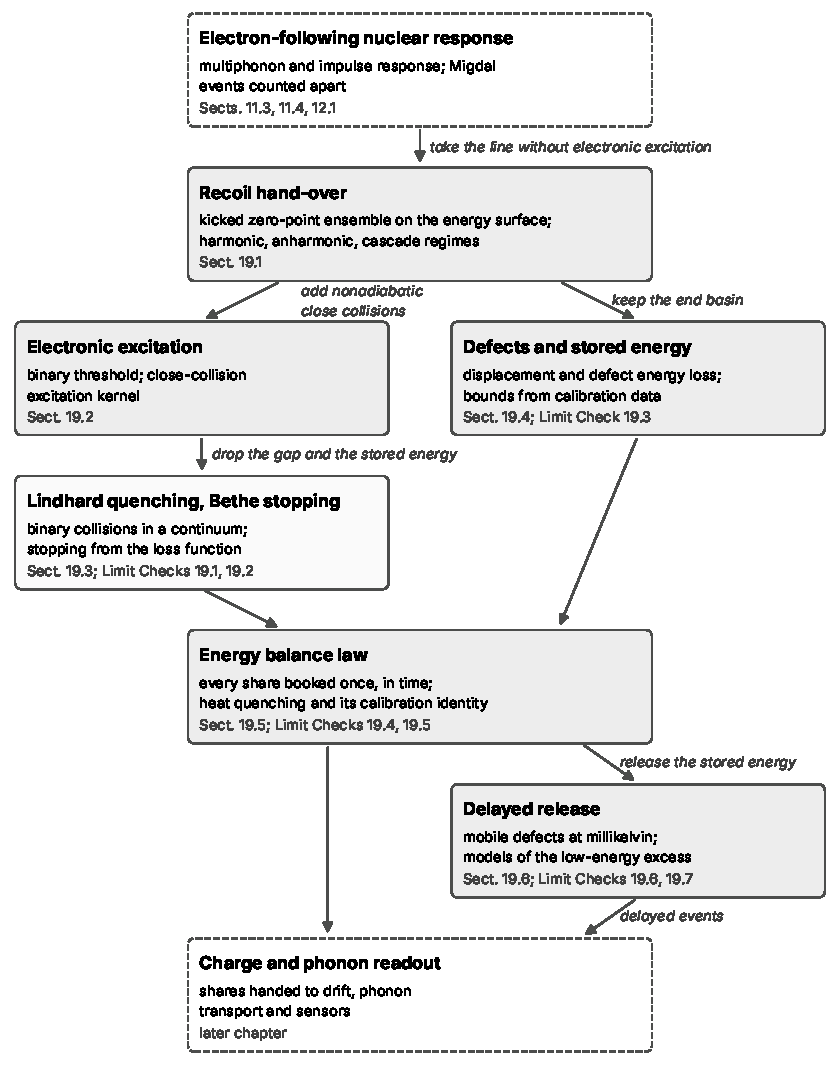
\includegraphics[width=0.85\linewidth]{figures/ch19/map19.pdf}
  \caption{Low-energy nuclear recoils, from the electron-following nuclear response (\cref{sec:11.3,sec:11.4}; Migdal events counted apart, \cref{sec:12.1-counting}) to the shares a detector reads. Main line: the hand-over of the kicked nucleus to dynamics on the Born--Oppenheimer surface, the regimes of that dynamics and the partition of the recoil energy into heat, stored energy and charge (\cref{sec:19.1}), then the energy balance law with heat quenching, its calibration identity and the bounds that calibration data set on the stored energy (\cref{sec:19.5}; \cref{lim:19.5a,lim:19.5b}). Left branch: electronic excitation in close collisions and the binary threshold (\cref{sec:19.2}), and Lindhard quenching and Bethe stopping as its limits (\cref{sec:19.3}; \cref{lim:19.3a,lim:19.3b}). Right branch: displacement and the energy stored in defects (\cref{sec:19.4}; \cref{lim:19.4a}), and the delayed release of that energy by mobile defects (\cref{sec:19.6}; \cref{lim:19.6a,lim:19.6b}), which feeds the readout as delayed events.}
  \label{fig:19-map}
\end{figure}

\section{Nuclear recoil on the Born--Oppenheimer surface}\label{sec:19.1}

A silicon nucleus kicked with \SI{12.5}{eV} along $\langle111\rangle$ either swings out and returns to its site, or pushes a neighbor into the open tetrahedral site and leaves a defect behind (\cref{sec:7.4}). The nuclear response of \cref{chap:11} does not distinguish the two outcomes. It gives the rate of the kick and the energy $\omega$ deposited, and both are fixed before the struck atom has moved (\cref{sec:11.4}). Which outcome occurs is decided afterward, in some \SI{25}{fs}, by the motion of the struck atom between its neighbors on the Born--Oppenheimer surface $E^{\mathrm{ad}}$ of \cref{sec:5.1}. To follow this motion we need the state in which the response leaves the crystal, the regimes in which that state can be propagated by classical dynamics, and a definition of the shares into which the energy finally splits.

\subsection{The hand-over from the nuclear response}\label{sec:19.1-handover}

The kick either leaves the electrons in their ground state or also excites them. On the plane of the joint response of \cref{sec:12.1}, the line $\omega_e = 0$ holds the kicks after which the electrons stay in their ground state. It has the weight $1 - P_{\mathrm{Mig}}(q)$ of \cref{eq:12.1-zeroth} and the dressed mass $M_\kappa + \delta M_\kappa$; the remaining kicks form the Migdal entry, in which the same kick also leaves an electronic energy $\omega_e > 0$ (\cref{sec:12.1-counting}). Kicks on the line $\omega_e = 0$ and Migdal events set the nucleus moving with the same lattice factor. We follow the nucleus here, and a Migdal event hands its electronic energy to the cascade of \cref{chap:18} in addition. In silicon the weight $1 - P_{\mathrm{Mig}}$ differs from one by less than $10^{-3}$ for $E_R \lesssim \SI{16}{eV}$ and by \SI{1.9}{\percent} at \SI{500}{eV} with the exact second-order bracket, \SI{3}{\percent} in the soft limit (\cref{sec:12.1-counting,sec:12.3-validity}).

At small recoil parameter $x_R = E_R/\langle\omega\rangle$ the final states of the line $\omega_e = 0$ are states of a few phonons, and the response already resolves them by branch and momentum (\cref{eq:11.3-Sn}). Their energy $\omega$ goes as heat straight to the phonon readout (\cref{sec:8.7}). At $T > 0$ some terms of the response absorb a thermal phonon instead of creating one; they carry negative heat, and the net lattice energy, created minus absorbed, is $\omega$.

At large $x_R$ the response no longer lists phonons. In the impulse regime it is a peak of width $\sigma_\omega$ around the free recoil energy $E_R = q^2/2M_\kappa$ (\cref{eq:11.4-IA}), and the nucleus that received the kick moves far enough to collide with its neighbors. The state of the lattice after the kick is known exactly. Within the Born--Oppenheimer approximation the kick acts on the nuclear wave function alone, and multiplies it by $\ee^{\ii\vect{q}\cdot\vect{X}_I}$, with $\vect{X}_I$ the position of the struck nucleus $I$ of species $\kappa$. Write $\{\vect{X}\}$ and $\{\vect{p}\}$ for the positions and momenta of all nuclei, and describe the initial state $\varrho_0$ of the lattice, ground or thermal, by its Wigner function
\begin{equation*}
  \mathcal{W}_0(\{\vect{X}\},\{\vect{p}\}) = \int\frac{\dd\{\vect{y}\}}{(2\pi)^{3N}}\;\langle\{\vect{X} - \vect{y}/2\}|\varrho_0|\{\vect{X} + \vect{y}/2\}\rangle\,\ee^{\ii\sum_J\vect{p}_J\cdot\vect{y}_J} ,
\end{equation*}
whose marginals are the distributions of the positions and of the momenta. After the kick the density matrix is $\ee^{\ii\vect{q}\cdot\vect{X}_I}\varrho_0\,\ee^{-\ii\vect{q}\cdot\vect{X}_I}$. Its matrix element between $\{\vect{X} - \vect{y}/2\}$ and $\{\vect{X} + \vect{y}/2\}$ is that of $\varrho_0$ times $\ee^{\ii\vect{q}\cdot(\vect{X}_I - \vect{y}_I/2)}\ee^{-\ii\vect{q}\cdot(\vect{X}_I + \vect{y}_I/2)} = \ee^{-\ii\vect{q}\cdot\vect{y}_I}$. The extra phase shifts the momentum variable of the Fourier integral:
\begin{equation}
  \mathcal{W}_+(\{\vect{X}\},\{\vect{p}\}) = \mathcal{W}_0(\{\vect{X}\},\{\vect{p}\})\big|_{\vect{p}_I \to \vect{p}_I - \vect{q}} .
  \label{eq:19.1-wigner}
\end{equation}
The kick leaves every position where it was and moves the momentum of one nucleus by $\vect{q}$, for any $q$ and any potential.

The Hamiltonian of the nuclei is $H = \sum_J\vect{p}_J^2/2M_J + E^{\mathrm{ad}}(\{\vect{X}\})$, a function of the momenta plus a function of the positions. For a Hamiltonian of this form, the phase-space function that represents $H$ in the Wigner picture is the classical $H_{\mathrm{cl}}(\{\vect{X}\},\{\vect{p}\})$ itself. Every point of phase space therefore gains
\begin{equation}
  H_{\mathrm{cl}}(\{\vect{X}\},\{\vect{p}\} + \vect{q}\hat{\vect{e}}_I) - H_{\mathrm{cl}}(\{\vect{X}\},\{\vect{p}\}) = E_R + \frac{\vect{q}\cdot\vect{p}_I}{M_\kappa} ,
  \label{eq:19.1-dH}
\end{equation}
with $\hat{\vect{e}}_I$ marking the momentum of nucleus $I$. This is the energy $D$ that the kick gives a free particle of momentum $\vect{p}_I$ (\cref{sec:11.4}). Now let each point of $\mathcal{W}_+$ move along its classical trajectory on $E^{\mathrm{ad}}$. Since classical motion conserves $H_{\mathrm{cl}}$, each trajectory carries its deposited energy \cref{eq:19.1-dH} unchanged, and the distribution of the deposit over the ensemble is the distribution of $E_R + \vect{q}\cdot\vect{p}_I/M_\kappa$ over the momentum marginal $\mathfrak{f}_\kappa(\vect{p}_I)$. This distribution is the impulse approximation \cref{eq:11.4-IA}, term by term.
\begin{keyresult}[Recoil hand-over]
In the impulse regime, the nuclear response hands over the ensemble $\mathcal{W}_+$ of \cref{eq:19.1-wigner}: positions and momenta drawn from the Wigner function of the lattice before the kick, ground or thermal, with the momentum of the struck nucleus raised by $\vect{q}$. Propagated classically on $E^{\mathrm{ad}}$, the ensemble deposits $\omega = E_R + \vect{q}\cdot\vect{p}_I/M_\kappa$ per trajectory, and the distribution of this deposit reproduces \cref{eq:11.4-IA} with its exact mean $E_R$ and its exact width $\sigma_\omega$ of \cref{eq:11.4-width}. The hand-over misses the third cumulant $c_3$ of \cref{eq:D.32-c3}, which carries the force of the neighbors during the kick, and the quantum corrections to the motion after the kick.
\end{keyresult}
\noindent The two omissions set the validity of the hand-over. The share of $c_3$ in the shape of the peak falls as $x_R^{-1/2}$ (\cref{sec:11.4}). The quantum corrections to the trajectories are small once the recoil holds many vibrational quanta. \Cref{sec:19.1-regimes} makes this condition quantitative, and in silicon it holds above about \SI{0.4}{eV}. For a harmonic lattice the Wigner function is a positive Gaussian, at the zero-point widths at $T = 0$ and with the $\coth(\omega/2T)$ widths of \cref{sec:11.4} at $T > 0$, and it can be sampled point by point. Anharmonic zero-point distributions come from path-integral sampling (\cref{app:E.17}).

The struck atom starts with a spread of kinetic energies. At $T = 0$ the spread is $\sigma_\omega = (E_R\langle\omega\rangle)^{1/2}$. For silicon at the lowest displacement threshold, $E_R = \SI{12.5}{eV}$ with $\langle\omega\rangle = \SI{40.9}{meV}$, $\sigma_\omega$ is \SI{0.72}{eV}, or \SI{5.7}{\percent} of the threshold. A simulation that starts the other atoms at rest, as for a classical crystal at millikelvin, has no spread of kinetic energies. The direction of the recoil is that of $\vect{q}$ only on average. Let $E^{\mathrm{kin}}_\kappa = \langle\omega\rangle/4 = \SI{10.2}{meV}$ be the mean zero-point kinetic energy of the nucleus per Cartesian component (\cref{sec:11.4}). The transverse momentum of the struck nucleus then has the rms value $(2M_\kappa E^{\mathrm{kin}}_\kappa)^{1/2}$ per component, against the kick $q = (2M_\kappa E_R)^{1/2}$, so the recoil direction scatters by the rms angle $(E^{\mathrm{kin}}_\kappa/E_R)^{1/2}$ in each transverse plane: \SI{1.6}{\degree} at \SI{12.5}{eV}, or \SI{2.3}{\degree} in polar angle. And the displacement threshold becomes a smooth step. Let $\hat{\vect{r}}_R = \hat{\vect{q}}$ be the recoil direction and run every trajectory of the ensemble until its motion has been carried off into the lattice. The basin of the perfect crystal on $E^{\mathrm{ad}}$ is the set of configurations that relax to it. The probability $p_{\mathrm{FP}}(E_R, \hat{\vect{r}}_R)$ that the end state lies outside this basin, in a Frenkel pair (FP) or another defect, rises from 0 to near 1 over a range of $E_R$, and we take as the displacement threshold the lowest $E_R$ at which $p_{\mathrm{FP}}$ reaches one half,
\begin{equation}
  E_{\mathrm{d}}(\hat{\vect{r}}_R) = \min\bigl\{E_R :\ p_{\mathrm{FP}}(E_R, \hat{\vect{r}}_R) \ge \tfrac12\bigr\} .
  \label{eq:19.1-Ed}
\end{equation}
When every trajectory of the ensemble is the same, $p_{\mathrm{FP}}$ is a step function and \cref{eq:19.1-Ed} is the deterministic threshold \cref{eq:7.4-Ed}. The spread $\sigma_\omega$ of the deposit spreads the step over about \SI{0.7}{eV} in silicon, before the spread of the initial positions adds its own; the measured onset of damage, $12.9 \pm \SI{0.6}{eV}$~\cite{loferski1958radiation}, carries an uncertainty of the same size. The step width is a prediction of the response and not a parameter of the dynamics. It matters for light dark matter, whose recoil spectrum falls steeply near its endpoint, so that the few recoils above $E_{\mathrm{d}}$ lie on the edge of the step.

\subsection{Regimes of the recoil dynamics}\label{sec:19.1-regimes}

Whether the handed-over ensemble may be propagated classically, harmonically, without defects and without electronic excitation is decided by four numbers: the quantum ratio $\lambda_{\mathrm{dB}}/\ell_R$, the anharmonic ratio $\eta_R$, the displacement threshold $E_{\mathrm{d}}$ and the Massey parameter $\xi_{\mathrm{M}}$. Each compares a property of the struck atom at kinetic energy $E_R$ with a scale of the crystal, and \cref{fig:19-recoil}(b) plots them for silicon.

The quantum and the anharmonic numbers use the amplitude of the struck atom's first excursion. Before its energy has spread, the atom moves in the cage of neighbors that have not yet responded, and for an estimate we treat that cage as an oscillator of the mean phonon frequency. The turning point of the struck atom lies at
\begin{equation*}
  \ell_R = \Bigl(\frac{2E_R}{M_\kappa\langle\omega\rangle^2}\Bigr)^{1/2} ,
\end{equation*}
from $E_R = \tfrac12M_\kappa\langle\omega\rangle^2\ell_R^2$. Classical mechanics holds when the de Broglie wavelength $\lambda_{\mathrm{dB}} = 2\pi/(2M_\kappa E_R)^{1/2}$ is short compared with this amplitude. The ratio is
\begin{equation*}
  \frac{\lambda_{\mathrm{dB}}}{\ell_R} = \frac{2\pi}{(2M_\kappa E_R)^{1/2}}\Bigl(\frac{M_\kappa\langle\omega\rangle^2}{2E_R}\Bigr)^{1/2} = \frac{\pi\langle\omega\rangle}{E_R} ,
\end{equation*}
independent of the mass: the motion is classical when the recoil holds many quanta $\langle\omega\rangle$. The corrections to classical trajectories are of second order in $\hbar$, and we take their relative size to be $(\lambda_{\mathrm{dB}}/\ell_R)^2$, an estimate. The harmonic approximation holds when $\ell_R$ is short compared with the length $3\Phi^{(2)}/|\Phi^{(3)}|$ over which the force constants change by their own size. The ratio of $\ell_R$ to this length is the anharmonic parameter $\eta_{\mathrm{anh}}$ of \cref{eq:5.7-eta} with the recoil amplitude in place of the zero-point length,
\begin{equation*}
  \eta_R = \frac{|\Phi^{(3)}|\,\ell_R}{3\Phi^{(2)}} ,
\end{equation*}
and by the counting of \cref{eq:5.7-order} the anharmonic corrections to energies and widths are of order $\eta_R^2$. For silicon, the bond-coordinate values of \cref{sec:5.7} give $3\Phi^{(2)}/|\Phi^{(3)}| = \SI{0.98}{\angstrom}$.

The third number is the displacement threshold itself: below $E_{\mathrm{d}}(\hat{\vect{r}}_R)$ the trajectory relaxes back into the basin of the perfect crystal, above it a defect survives with probability $p_{\mathrm{FP}}$. The fourth number decides whether the electrons follow. A nucleus at speed $v_N = (2E_R/M_\kappa)^{1/2}$ changes the potential seen by the electrons over a time $\ell_{\mathrm{int}}/v_N$, with $\ell_{\mathrm{int}} \approx \SI{1}{\angstrom}$ the range over which a close collision distorts the bonds. The electrons follow adiabatically if this time is long compared with $1/\Eg$, the time scale of the lowest excitation. The ratio of the two times is the Massey parameter
\begin{equation*}
  \xi_{\mathrm{M}} = \frac{\Eg\,\ell_{\mathrm{int}}}{v_N} ,
\end{equation*}
and for a perturbation that is smooth on the scale $\ell_{\mathrm{int}}$ the probability of an electronic transition falls as $\ee^{-\xi_{\mathrm{M}}}$. The bulk gap overstates the adiabaticity of a close collision, since the local gap of the compressed pair closes as the atoms approach, and \cref{sec:19.2} treats electronic excitation in close collisions.

\begin{figure}[tbp]
  \centering
  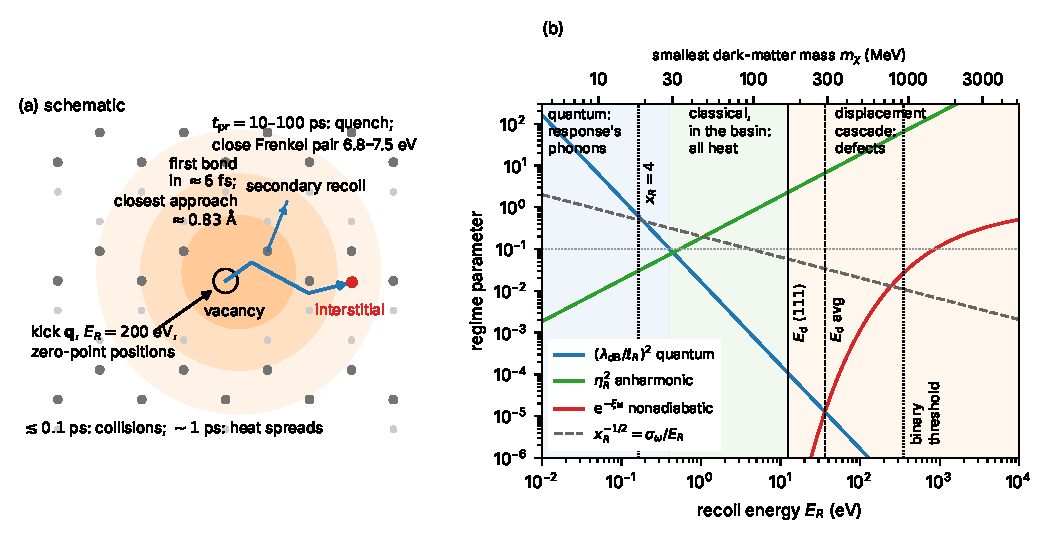
\includegraphics[width=\linewidth]{figures/ch19/fig19_1.pdf}
  \caption{A silicon nuclear recoil after the hand-over. (a) Schematic of a \SI{200}{eV} recoil in a $(1\bar10)$ plane of the diamond lattice (dark dots: atoms in the plane; light dots: the neighboring planes). The kick starts the struck atom from its zero-point position; it crosses its first bond in about \SI{6}{fs}, with a closest approach of \SI{0.83}{\angstrom} in a head-on collision, and sets a secondary atom moving. Within about \SI{0.1}{ps} the collisions are over, and within about a picosecond the heat (shaded rings) spreads through the crystal. At the partition time $t_{\mathrm{pr}}$ of \cref{sec:19.1-partition}, 10 to \SI{100}{ps}, the end state is quenched: here a vacancy and an interstitial, which as a close Frenkel pair store 6.8 to \SI{7.5}{eV}. Paths and end positions are drawn by hand. (b) The regime parameters against the recoil energy $E_R$ at $T = 0$. Curves: the quantum correction $(\lambda_{\mathrm{dB}}/\ell_R)^2 = (\pi\langle\omega\rangle/E_R)^2$, the anharmonic parameter $\eta_R^2$ with $3\Phi^{(2)}/|\Phi^{(3)}| = \SI{0.98}{\angstrom}$, the adiabatic suppression $\ee^{-\xi_{\mathrm{M}}}$ with $\Eg = \SI{1.17}{eV}$ and $\ell_{\mathrm{int}} = \SI{1}{\angstrom}$, and the relative width $x_R^{-1/2} = \sigma_\omega/E_R$ of the handed-over deposit, with $\langle\omega\rangle = \SI{40.9}{meV}$. The dotted horizontal line is the criterion 0.1. Vertical lines: impulse onset $x_R = 4$, displacement thresholds \SI{12.5}{eV} ($\langle111\rangle$) and \SI{36}{eV} (Frenkel pair, direction average), and the binary electron--hole threshold \SI{352}{eV} of \cref{sec:19.2}. Shading: quantum regime, where the phonons of the response are the final state (blue); classical motion inside the basin of the perfect crystal, where all energy becomes heat (green); displacement cascade (orange). Top axis: the smallest dark-matter mass that reaches $E_R$ at $v_{\mathrm{max}} = 2.650\times10^{-3}$.}
  \label{fig:19-recoil}
\end{figure}

The numbers divide the recoil energies into a quantum, a classical, a displacement and a nonadiabatic regime. The boundaries between the regimes follow from the definitions of the four numbers. Their positions depend on the criterion and on the cage estimate, and we quote them as estimates for a criterion of 0.1.
\begin{description}
\item[Quantum.] For $(\pi\langle\omega\rangle/E_R)^2 > 0.1$, that is $E_R < \pi\langle\omega\rangle/\sqrt{0.1}$, the recoil holds too few quanta for classical motion. The response is the whole answer here: its phonons are the final state and the energy is heat.
\item[Classical, inside the basin.] From the upper edge of the quantum regime up to $E_{\mathrm{d}}$ the motion is classical and adiabatic, anharmonic above $\eta_R^2 = 0.1$, and the trajectory relaxes back to the perfect crystal. Born--Oppenheimer molecular dynamics is controlled, and all of the energy becomes heat. The dynamics adds to the response the spectrum of the phonons the recoil leaves, which anharmonic collisions redistribute.
\item[Displacement cascade.] Above $E_{\mathrm{d}}$ some trajectories end in a defect, and the energy splits into heat and stored energy. A recoil many times $E_{\mathrm{d}}$ sets secondary atoms moving above their own thresholds and so starts the collision cascade of \cref{fig:19-recoil}(a).
\item[Nonadiabatic.] Where $\ee^{-\xi_{\mathrm{M}}}$ is no longer negligible, the electrons are excited along the path, and part of the energy becomes charge.
\end{description}
The quantum and harmonic boundaries lie close together: in silicon there is no wide window in which the motion is both harmonic and classical. The hand-over, however, does not need the motion to be harmonic. It takes place at the instant of the kick, and its only requirement on the later motion is that the motion be classical.

\begin{workedexample}{Regime boundaries for silicon}\label{we:19-boundary}
A silicon nucleus of the natural isotope mixture has $M_\kappa = 28.0855\,\mathrm{u} = \SI{26.16}{GeV}$, as in \cref{sec:5.3}, and $\langle\omega\rangle = \SI{40.9}{meV}$ (\cref{sec:11.4}). The cage stiffness is $M_\kappa\langle\omega\rangle^2 = \SI{26.16}{GeV}\times(\SI{0.0409}{eV})^2/(\hbar c)^2 = \SI{11.24}{eV.\angstrom^{-2}}$, with $\hbar c = \SI{1973.27}{eV.\angstrom}$.

\emph{Classical boundary.} $(\pi\langle\omega\rangle/E_R)^2 = 0.1$ gives $E_R = \pi\times\SI{0.0409}{eV}/0.316 = \SI{0.41}{eV}$, or $x_R = 9.9$. At \SI{1}{eV}, $\lambda_{\mathrm{dB}} = \SI{0.054}{\angstrom}$ against $\ell_R = \SI{0.42}{\angstrom}$, and the correction estimate is 0.017.

\emph{Harmonic boundary.} $\eta_R^2 = 0.1$ means $\ell_R = 0.316\times\SI{0.98}{\angstrom} = \SI{0.31}{\angstrom}$, reached at $E_R = \tfrac12\times\SI{11.24}{eV.\angstrom^{-2}}\times(\SI{0.31}{\angstrom})^2 = \SI{0.54}{eV}$. At \SI{1}{eV}, $\eta_R^2 = 0.18$.

\emph{Displacement.} The lowest threshold is \SI{12.5}{eV} along $\langle111\rangle$, the direction average for a Frenkel pair \SI{36}{eV}~\cite[Table~IV]{holmstrom2008threshold}. At \SI{12.5}{eV} the cage amplitude is $\ell_R = \SI{1.49}{\angstrom}$, more than half the bond length of \SI{2.35}{\angstrom}: the cage estimate has run out, as it should, since the atom is leaving its cage. The atom moves at $v_N = \SI{9.27}{km/s}$ and crosses one bond in \SI{25}{fs}, less than half the shortest phonon period of \SI{65}{fs} ($2\pi/\omega_{\mathrm{opt}}$ with $\omega_{\mathrm{opt}} = \SI{64.1}{meV}$, \cref{sec:5.7}), so the collision is over before the lattice has responded. The energy ends in some $\SI{12.5}{eV}/\langle\omega\rangle \approx 300$ phonons if no defect survives.

\emph{Adiabaticity.} At \SI{20}{eV}, $v_N = \SI{11.7}{km/s}$ and $\xi_{\mathrm{M}} = \SI{1.17}{eV}\times\SI{1}{\angstrom}/(\hbar v_N) = 15$, with $\hbar = \SI{6.582e-16}{eV.s}$, so $\ee^{-\xi_{\mathrm{M}}} = 3\times10^{-7}$. Since $\xi_{\mathrm{M}} \propto E_R^{-1/2}$, the suppression reaches 0.1 ($\xi_{\mathrm{M}} = 2.3$) at \SI{0.87}{keV}, and $\xi_{\mathrm{M}} = 1$ at \SI{4.6}{keV}.

\emph{Dark-matter masses.} By \cref{eq:1.3-ERmax} with $v_{\mathrm{max}} = 2.650\times10^{-3}$, the classical boundary needs $\mchi \ge \SI{28}{MeV}$, the harmonic boundary \SI{32}{MeV}, the lowest threshold \SI{154}{MeV}, the average threshold \SI{262}{MeV}, and $\ee^{-\xi_{\mathrm{M}}} = 0.1$ needs \SI{1.3}{GeV}.
\end{workedexample}


\subsection{Acceptance tests for recoil molecular dynamics}\label{sec:19.1-md}

In the classical regimes the handed-over ensemble is propagated by molecular dynamics on $E^{\mathrm{ad}}$. A recoil cascade needs cells of thousands of atoms and thousands of trajectories, far beyond direct density-functional dynamics. In practice the surface is therefore a machine-learned interatomic potential, trained on density-functional energies and forces and joined to a screened Coulomb repulsion at short distance. \Cref{app:E.11} describes the method.

The energy surface must be right along the path of the struck atom, not only near equilibrium. The threshold is set by the energy surface between the neighbors that the struck atom squeezes past. Potentials that agree on elastic constants and defect energies can still disagree on thresholds by several eV; the Stillinger--Weber potential overshoots the density-functional threshold along $\langle111\rangle$ by 4 to \SI{6}{eV} (\cref{sec:7.4}). The accuracy target is the width of the step in $p_{\mathrm{FP}}$, about \SI{0.7}{eV} at the lowest silicon threshold, checked against density-functional dynamics along a few directions. Closer in, the closest approach of a head-on collision is \SI{1.49}{\angstrom} at \SI{20}{eV} and \SI{0.83}{\angstrom} at \SI{200}{eV} (\cref{tab:E-md-si}). At these distances the screened Coulomb repulsion dominates, and the splice between the machine-learned potential and the screened Coulomb repulsion must be complete above the turning point of threshold collisions, so that the dynamics near $E_{\mathrm{d}}$ never feels the splice.

The initial ensemble must be the kicked zero-point ensemble of the hand-over, not a lattice at rest. Classical propagation of a Wigner ensemble is exact for a quadratic Hamiltonian, since the quantum evolution of the Wigner function then reduces to the classical Liouville flow. The zero-point motion of the parts of the crystal that stay harmonic is therefore carried correctly. Where the collision makes the surface anharmonic, classical dynamics lets the zero-point energy of one mode flow into others and leaves the mode below its quantum ground state, a state that quantum dynamics forbids. The error from this leakage is of the order of the zero-point energy of the atoms the collision disturbs, a few tens of meV each, and the definition of the stored energy below is built so that the error does not enter.

The stored energy must be measured between minima. On average, each atom of the initial ensemble lies above the minimum of $E^{\mathrm{ad}}$ by half its zero-point energy, $3\langle\omega\rangle/4 = \SI{31}{meV}$ per atom in silicon (the zero-point energy of \cref{sec:5.3} is \SI{123}{meV} per cell of two atoms). In a cell of 4096 atoms this excess is \SI{126}{eV}, more than ten times the energy of a Frenkel pair. The end state and the perfect crystal are therefore both relaxed to their minima, by a quench at fixed cell without annealing, and the stored energy is the difference \cref{eq:E.11-Est}. The potential's own error on defect energies sets a floor: a potential whose formation energies lie within \SI{7}{\percent} of density-functional theory~\cite[Sect.~III\,E]{bartok2018machine} carries an error of a few tenths of an eV on a defect that stores several eV. One table of these minimum energies, with one potential and cell, must serve the stored energy of \cref{sec:19.4} and the release paths of \cref{sec:19.6}, or the two disagree by that error.

The harmonic limit provides an acceptance test. With $E^{\mathrm{ad}}$ replaced by its harmonic expansion, the classical propagation of $\mathcal{W}_+$ is exact. The mean energy that the kick leaves in a normal mode $s$ is then $|\vect{q}\cdot\vect{e}_{\kappa s}|^2/2NM_\kappa$, with $\vect{e}_{\kappa s}$ the polarization vector of the mode on the struck site and $N$ the number of cells. It is half the square of the mass-weighted momentum the kick gives the mode, since the cross term with the mode's own momentum averages to zero over the ensemble. These mode energies sum to $E_R$ by the completeness of the polarization vectors, and they are the energy-weighted phonon content of the harmonic response of \cref{sec:11.3} at the same $\vect{q}$. A calculation that propagates the kicked ensemble on the true surface must recover this spectrum for recoils small enough to stay harmonic, and the mean and width of \cref{eq:11.4-IA} for all others.

The electronic channel is missing from Born--Oppenheimer dynamics. A common remedy adds a friction force, minus the electronic stopping power times the direction of motion. Below the binary threshold of \cref{sec:19.2} that friction fails (\cref{sec:19.3-assumptions}), and at any energy it supplies a mean loss without its distribution. Where the electronic channel matters, the friction is replaced by excitation events drawn at each close collision from a kernel computed with time-dependent density-functional theory (\cref{sec:19.2}).

\subsection{Partition of the recoil energy}\label{sec:19.1-partition}

The shares of the recoil energy change with time, and the partition needs a time. The collisions are over within about \SI{0.1}{ps}, and the hot carriers that the recoil excites finish their cascade within a picosecond (\cref{chap:18}). Defects at millikelvin, on the other hand, cannot cross barriers of chemical size by thermal activation, since a barrier of \SI{0.1}{eV} at \SI{10}{mK} carries the Boltzmann factor $\ee^{-1.2\times10^5}$ (\cref{sec:7.4}); they move only by tunneling or with the phonons of later events (\cref{sec:19.6}). The drift of the pairs to the electrodes takes longer still (\cref{sec:20.1}). Any time $t_{\mathrm{pr}}$ between 10 and \SI{100}{ps} after the recoil comes after the collisions and the hot-carrier cascade and before any defect motion or pair drift, and we fix the partition there.

At $t_{\mathrm{pr}}$ the energy $\omega$ deposited in the kick has gone three ways. Part has gone to the electrons: the energy $\omega_e$ of a Migdal event, if the kick was one, plus whatever the moving nucleus excited along its path. The nuclei keep the rest of $\omega$, as kinetic energy and as potential energy on $E^{\mathrm{ad}}$. The quench at $t_{\mathrm{pr}}$ splits the nuclear share into the energy of the minimum that the crystal has reached and the vibrational energy about that minimum.
\begin{keyresult}[Partition of the recoil energy]
At the time $t_{\mathrm{pr}}$,
\begin{equation}
  \omega = E_{\mathrm{lat}} + E_{\mathrm{st}} + \omega_e , \qquad
  E_{\mathrm{st}} = E^{\mathrm{ad}}_{\mathrm{min}}(\mathrm{end}) - E^{\mathrm{ad}}_{\mathrm{min}}(\mathrm{perfect}) ,
  \label{eq:19.1-partition}
\end{equation}
where $\omega_e$ is the energy given to the electrons and $E_{\mathrm{st}}$ the stored energy, the difference of the minima of $E^{\mathrm{ad}}$ in the basin of the end state and in that of the perfect crystal. The lattice share $E_{\mathrm{lat}}$ is the vibrational energy in excess of the zero-point energy of the perfect crystal. After the cascade of \cref{chap:18} has turned $\omega_e$ into $N_{\mathrm{eh}}$ pairs,
\begin{equation}
  \omega = N_{\mathrm{eh}}\Eg + E_{\mathrm{heat}} + E_{\mathrm{st}} , \qquad
  E_{\mathrm{heat}} = E_{\mathrm{lat}} + \bigl(\omega_e - N_{\mathrm{eh}}\Eg\bigr) .
  \label{eq:19.1-heat}
\end{equation}
\end{keyresult}
\noindent The energy balance follows from the conservation of the total energy along each trajectory. Before the kick the nuclei hold the minimum of the perfect crystal and its zero-point energy; the kick adds $\omega$, and the electrons take away $\omega_e$. At $t_{\mathrm{pr}}$ the nuclei hold the minimum of the end basin and the vibrational energy about it, and subtracting the balance before the kick from the balance at $t_{\mathrm{pr}}$ gives \cref{eq:19.1-partition}. The second form uses the cascade identity \cref{eq:18.1-energy} for each electronic excitation, $\omega_e = N_{\mathrm{eh}}\Eg + E_{\mathrm{heat}}$ of the cascade, and collects all phonon energy, from the lattice and from the cascade, in one $E_{\mathrm{heat}}$. For an electronic deposit, with $E_{\mathrm{lat}} = E_{\mathrm{st}} = 0$, the second form is \cref{eq:18.1-energy} itself. Capture at the end of the cascade moves energy out of the pairs as in \cref{sec:18.5}.

The stored energy is configurational: it compares minima of $E^{\mathrm{ad}}$ and contains no vibrational energy. The zero-point energy of the end basin differs from that of the perfect crystal, since a defect softens or stiffens the modes around it, and the difference is part of $E_{\mathrm{lat}}$, on the vibrational side. This zero-point difference is part of the heat but cannot reach a sensor, and \cref{sec:19.5} counts it separately. The stored energy is also not the displacement threshold, which is a barrier on the path rather than a difference of end points. A close Frenkel pair keeps about half of the lowest silicon threshold, and the rest of the threshold energy becomes heat (\cref{sec:7.4}).

The partition is random. Each trajectory of the handed-over ensemble ends with its own $(E_{\mathrm{lat}}, E_{\mathrm{st}}, \omega_e)$, and in the impulse regime the ensemble is fixed by $E_R$, the direction $\hat{\vect{r}}_R$ and the temperature. The cascade turns the electronic excitations into pairs with the distribution $P_{\mathrm{casc}}$ of \cref{sec:18.3}, evaluated at the seed energies the recoil produced, which lie near the gap. The result is a joint distribution $P(E_{\mathrm{heat}}, E_{\mathrm{st}}, N_{\mathrm{eh}}|E_R, \hat{\vect{r}}_R, T)$. Its correlations matter as much as its means, since a recoil that stores energy in a defect leaves less heat and, through the same collision, may give fewer pairs.

Below $E_{\mathrm{d}}$ the adiabatic suppression makes $\omega_e$ negligible, $\ee^{-\xi_{\mathrm{M}}} = 5\times10^{-9}$ at \SI{12.5}{eV}, and every trajectory returns to the perfect crystal, so the recoil deposits all of its energy as heat. In silicon the recoils below $E_{\mathrm{d}}$ include every electron-following recoil from dark matter below about \SI{150}{MeV} (\cref{we:19-boundary}). The charge that these recoils produce therefore comes from the Migdal entry of the response and from the soft tail of electronic excitation of \cref{sec:19.2}, not from the recoil dynamics. After $t_{\mathrm{pr}}$ the stored energy decreases as defects release it, and the pairs recombine or are collected; the balance law of \cref{sec:19.5} carries this time dependence, with \cref{eq:19.1-partition} as its starting point.

\section{Electronic excitation by the recoil}\label{sec:19.2}

A silicon nucleus recoiling with \SI{100}{eV} moves at \SI{26}{km/s}, eighty times slower than the valence electrons at the Fermi velocity. A neutron calibration finds that such recoils leave on average 2.7 electron--hole pairs, an ionization yield of $0.102^{+0.034}_{-0.030}$~\cite[Table~II]{albakry2023first}. Yet a binary collision between the nucleus and a valence electron cannot create a single pair until the recoil carries about \SI{350}{eV}. The charge at \SI{100}{eV} must therefore come from processes that the binary picture leaves out, and these are the processes that set the charge signal of light dark matter, whose nuclear recoils in silicon stay below \SI{100}{eV} for masses under \SI{0.44}{GeV}. The question is which processes those are, and how much of the charge the Migdal effect of \cref{chap:12} already supplies.

\subsection{The binary electron--hole threshold}\label{sec:19.2-binary}

The recoiling ion is a projectile of the master formula, as the hot carrier of \cref{sec:18.1} was. It couples to the electron density through its screened charge, and the energy it hands to the electrons at momentum $\vect{k}$ is $\omega = \vect{k}\cdot\vect{v}_N - k^2/2M_\kappa \le kv_N$, with $v_N = q/M_\kappa$ the nuclear velocity after the kick. The stopping power \cref{eq:4.4-dEdx} contains this constraint as the upper limit $\omega \le kv_N$ of its inner integral; \cref{sec:19.3} evaluates that integral.

Consider first a free electron gas with the valence density of the crystal and a gap $\Eg$ added by hand. Its loss function vanishes outside the particle--hole continuum of \cref{sec:4.2}, which for $k > 2k_{\mathrm{F}}$ begins at $\omega_-(k) = k^2/2m_e - kv_{\mathrm{F}}$. An electron--hole pair needs $\omega \ge \Eg$, and the ion supplies at most $\omega = kv_N$. Both conditions hold at some $k$ only if the line $\omega = kv_N$ rises above $\omega_-(k)$ at an energy of at least $\Eg$. The line and the edge cross at $k = 2m_e(v_N + v_{\mathrm{F}})$, where $\omega = 2m_ev_N(v_N + v_{\mathrm{F}})$, and this is the largest energy the ion can deposit in one electronic excitation:
\begin{equation}
  \omega_{\mathrm{max}} = 2m_e v_N\,(v_N + v_{\mathrm{F}}) .
  \label{eq:19.2-transfer}
\end{equation}
The same number follows from a collision of two particles. In the rest frame of the heavy ion an electron moving against it at $v_{\mathrm{F}}$ approaches with speed $v_{\mathrm{F}} + v_N$ and is reflected with the same speed, and in the crystal frame it leaves with $v_{\mathrm{F}} + 2v_N$. Its kinetic energy rises by $\tfrac12 m_e[(v_{\mathrm{F}} + 2v_N)^2 - v_{\mathrm{F}}^2]$, which is \cref{eq:19.2-transfer}. The heavy ion acts as a moving wall: it reverses the electron's velocity in its own frame, and the energy it gives is linear in $v_N$.

Setting $\omega_{\mathrm{max}} = \Eg$ gives the threshold speed. Since $v_N \ll v_{\mathrm{F}}$ at every recoil energy of interest, the term $v_N^2$ can be dropped.

\begin{keyresult}[Binary electron--hole threshold]
A slow ion creates an electron--hole pair in a binary collision with a free-electron-like valence band only above the speed $v_{N,\mathrm{th}} = \Eg/(2m_ev_{\mathrm{F}})$, that is, above the recoil energy
\begin{equation}
  E_{R,\mathrm{th}} = \frac12 M_\kappa v_{N,\mathrm{th}}^2 = \frac{M_\kappa}{m_e}\,\frac{\Eg^2}{16E_{\mathrm{F}}} ,
  \label{eq:19.2-Eth}
\end{equation}
with $E_{\mathrm{F}} = m_ev_{\mathrm{F}}^2/2$ the Fermi energy of the valence electrons. It is \SI{352}{eV} in silicon and \SI{399}{eV} in germanium.
\end{keyresult}

The threshold is the gap multiplied by two numbers, the mass ratio $M_\kappa/m_e$, which is large, and $\Eg/16E_{\mathrm{F}}$, which is small. In silicon the product puts $E_{R,\mathrm{th}}$ at three hundred times the gap. Keeping the term $v_N^2$ in \cref{eq:19.2-transfer} and solving the quadratic, $v_N = \tfrac12[(v_{\mathrm{F}}^2 + 2\Eg/m_e)^{1/2} - v_{\mathrm{F}}]$, lowers the threshold by \SI{4.4}{\percent} to \SI{336}{eV} in silicon and by \SI{3.1}{\percent} to \SI{387}{eV} in germanium. For germanium we use $\Eg = \SI{0.744}{eV}$ and $a = \SI{5.658}{\angstrom}$ (\cref{sec:3.3}), so that $k_{\mathrm{F}} = \SI{1.736}{\angstrom^{-1}}$, $E_{\mathrm{F}} = \SI{11.48}{eV}$ and $M_\kappa/m_e = \num{132396}$. The heavier nucleus raises the threshold, and the smaller gap, which enters squared, lowers it again.

\begin{workedexample}{The binary threshold of silicon}\label{we:19-threshold}
Silicon has four valence electrons per atom and eight atoms in the cubic cell of side $a = \SI{5.431}{\angstrom}$, so the valence density is $\nd_e = 32/a^3 = \SI{0.19976}{\angstrom^{-3}}$. The free-electron Fermi wavevector is $k_{\mathrm{F}} = (3\pi^2\nd_e)^{1/3} = \SI{1.8085}{\angstrom^{-1}}$, or $k_{\mathrm{F}} = \SI{1.8085}{\angstrom^{-1}}\times\SI{1973.27}{eV\,\angstrom} = \SI{3.569}{keV}$, as in \cref{fig:4-gas}. Then
\begin{equation*}
  E_{\mathrm{F}} = \frac{k_{\mathrm{F}}^2}{2m_e} = \frac{(\SI{3.569}{keV})^2}{2\times\SI{511.0}{keV}} = \SI{12.46}{eV} , \qquad
  v_{\mathrm{F}} = \frac{k_{\mathrm{F}}}{m_e} = 6.984\times10^{-3} = \SI{2094}{km/s} .
\end{equation*}
With the low-temperature gap $\Eg = \SI{1.17}{eV}$ the threshold speed is $v_{N,\mathrm{th}} = \Eg/(2m_ev_{\mathrm{F}}) = \SI{1.17}{eV}/(2\times\SI{511.0}{keV}\times6.984\times10^{-3}) = 1.639\times10^{-4}$, or \SI{49.2}{km/s}. The silicon nucleus has $M_\kappa = 28.0855\times\SI{931.494}{MeV} = \SI{26.16}{GeV}$, so $M_\kappa/m_e = \num{51197}$, and
\begin{equation*}
  E_{R,\mathrm{th}} = \frac{M_\kappa}{m_e}\,\frac{\Eg^2}{16E_{\mathrm{F}}} = \num{51197}\times\frac{(\SI{1.17}{eV})^2}{16\times\SI{12.46}{eV}} = \num{51197}\times\SI{6.87e-3}{eV} = \SI{352}{eV} .
\end{equation*}
For comparison, \cref{eq:19.2-transfer} at $E_R = \SI{100}{eV}$, where $v_N = 8.74\times10^{-5}$, gives $\omega_{\mathrm{max}} = \SI{0.63}{eV}$: about half the gap, too little for a binary collision at the measured \SI{100}{eV} point to make a pair. Dark matter needs a mass of at least \SI{0.84}{GeV} to give a nucleus \SI{352}{eV} (\cref{sec:19.1}).
\end{workedexample}

\subsection{Softening by the valence momentum tail}\label{sec:19.2-soft}

\Cref{eq:19.2-Eth} assumed that no valence electron moves faster than $v_{\mathrm{F}}$. In a crystal this is not so. A Bloch state of crystal momentum $\vect{k}$ has components at every $\vect{k} + \vect{G}$, and near each nucleus the valence orbitals oscillate to stay orthogonal to the core; as a result the valence momentum density extends beyond $k_{\mathrm{F}}$. An electron of momentum $p$ moving against the ion gains up to $2m_ev_N(v_N + p/m_e)$, and it can be promoted across the gap if
\begin{equation}
  p \ge p_{\mathrm{min}}(E_R) = \frac{\Eg}{2v_N} - m_ev_N , \qquad v_N = (2E_R/M_\kappa)^{1/2} .
  \label{eq:19.2-pmin}
\end{equation}
In the free gas the fraction of valence electrons above $p_{\mathrm{min}}$ is $1 - (p_{\mathrm{min}}/k_{\mathrm{F}})^3$, which vanishes where $p_{\mathrm{min}} = k_{\mathrm{F}}$, at the threshold with $v_N^2$ kept, \SI{336}{eV}. In silicon at \SI{100}{eV}, $p_{\mathrm{min}} = \SI{3.37}{\angstrom^{-1}} = 1.86\,k_{\mathrm{F}}$. In the language of the loss function, the free-gas support ends at $\omega_-(k)$ and the crystal's $L(\vect{k},\omega)$ at $k \gtrsim 2k_{\mathrm{F}}$ and $\omega \ge \Eg$ is the low-energy tail of the Bethe ridge $\omega \approx k^2/2m_e$, whose width is set by the momentum distribution of the valence electrons. The tail is small but not zero; below $E_{R,\mathrm{th}}$ the linear-response excitation is therefore suppressed, not forbidden.

\Cref{fig:19-yield}(b) shows how much the tail changes the count. It compares the free-gas fraction with the same fraction computed from the valence momentum density of the empirical pseudopotential model of \cref{sec:3.3}, summed over the four valence bands on a $10^3$ grid of the zone. In the model, \SI{23}{\percent} of the valence momentum density lies beyond $k_{\mathrm{F}}$, \SI{2.2}{\percent} beyond $1.5\,k_{\mathrm{F}}$ and \SI{0.34}{\percent} beyond $2k_{\mathrm{F}}$. The fraction of electrons fast enough to be promoted falls smoothly through $E_{R,\mathrm{th}}$ instead of vanishing there: it is 0.27 at \SI{352}{eV}, where the free gas has 0.07, then 0.047 at \SI{200}{eV}, $5.6\times10^{-3}$ at \SI{100}{eV} and $4\times10^{-4}$ at \SI{50}{eV}. The model's pseudo-orbitals are smooth inside the cores, where the true valence orbitals oscillate, and its plane waves stop at \SI{5.3}{\angstrom^{-1}}, close to $p_{\mathrm{min}}$ at \SI{50}{eV}; its tail is therefore smaller than the real one, and the numbers indicate the shape of the softening, not its size. The fraction is also not yet a yield: an electron above $p_{\mathrm{min}}$ is promoted only in a head-on encounter, and the conduction states must accept it.

The zero-point momentum of the struck nucleus spreads its recoil energy by about \SI{2}{eV} at $E_R = \SI{100}{eV}$ (\cref{sec:19.1}), which is negligible against \SI{352}{eV}.

\subsection{Close collisions and the excitation kernel}\label{sec:19.2-kernel}

Within a few femtoseconds a recoil of a few hundred eV strikes a neighbor, closer than a bond length, and passes on part of its energy; the neighbor strikes the next atom, and so on (\cref{sec:19.1}). In such an encounter two atoms come within an angstrom of each other, and the electrons around them briefly belong to a quasi-molecule, Si$_2$ or Ge$_2$, whose levels depend on the distance between the nuclei. The bulk gap no longer sets the excitation threshold. As the nuclei approach, a filled level and an empty one can cross, or nearly cross, and an electron can be promoted at the crossing.

How likely that is depends on how fast the crossing is passed. Away from crossings the Massey parameter $\xi_{\mathrm{M}} = \Eg\ell_{\mathrm{int}}/v_N$ of \cref{sec:19.1} measures adiabaticity, and nonadiabatic excitation is suppressed roughly as $\ee^{-\xi_{\mathrm{M}}}$; in silicon, with $\ell_{\mathrm{int}} = \SI{1}{\angstrom}$, $\xi_{\mathrm{M}}$ is 6.8 at $E_R = \SI{100}{eV}$, 3.6 at $E_{R,\mathrm{th}}$ and 2.1 at \SI{1}{keV}. At an avoided crossing the relevant gap is the local splitting $2h_{\mathrm{LZ}}$ of the two levels, with $h_{\mathrm{LZ}}$ the coupling between the crossing diabatic states. The relevant speed is the rate $v|\Delta F_{\mathrm{LZ}}|$ at which their energy difference sweeps through zero, where $v$ is the relative speed of the nuclei and $\Delta F_{\mathrm{LZ}}$ the difference of the slopes of the two diabatic levels against the internuclear distance. The electrons jump from the lower adiabatic level to the upper one in one passage with the Landau--Zener probability~\cite{zener1932non,vutha2010simple}
\begin{equation}
  P_{\mathrm{LZ}} = \exp\!\left(-\frac{2\pi h_{\mathrm{LZ}}^2}{v\,|\Delta F_{\mathrm{LZ}}|}\right) .
  \label{eq:19.2-LZ}
\end{equation}
A collision passes each crossing twice, on the way in and on the way out. If the phase between the two passages is averaged over impact parameters, the electrons end up excited with probability $2P_{\mathrm{LZ}}(1 - P_{\mathrm{LZ}})$, one jump and one adiabatic passage in either order. Unlike $\ee^{-\xi_{\mathrm{M}}}$, \cref{eq:19.2-LZ} is set by the small splitting at the crossing, not by the bulk gap, and it is why close collisions can excite electrons well below $E_{R,\mathrm{th}}$.

The excitation cannot be computed in linear response in the ion's charge. The Born parameter of the collision, $Z_\kappa\alpha/v_{\mathrm{F}}$, is 15 for silicon and 35 for germanium. The ion's own electrons screen its charge, but the parameter exceeds one already for a unit charge, and the ion perturbs the electrons near it strongly; and the Massey parameter near \SI{1}{keV} is of order one, so the electrons neither follow adiabatically nor stay frozen. The excitation is instead described by a kernel tabulated from a nonperturbative calculation. It is the distribution
\begin{equation}
  \frac{\dd P}{\dd\omega_e}(b_{\mathrm{imp}}, E_{\mathrm{coll}})
  \label{eq:19.2-kernel}
\end{equation}
of the electronic excitation energy $\omega_e$ left behind when two Si or two Ge atoms collide in the crystal at impact parameter $b_{\mathrm{imp}}$ and relative energy $E_{\mathrm{coll}}$, in units of eV$^{-1}$. Its integral over $\omega_e$ is the probability that the collision excites the electrons. Along the trajectory of a recoil, every close approach $j$ draws an excitation from the kernel at its own $(b_j, E_j)$; with the trajectories of the partition of \cref{sec:19.1}, this gives the excitation spectrum of the whole recoil, $\dd\mathcal{N}_{\mathrm{exc}}/\dd\omega_e = \langle\sum_j(\dd P/\dd\omega_e)(b_j, E_j)\rangle$. The spectrum has three parts, which a calculation should keep apart: binary excitation above $E_{R,\mathrm{th}}$, promotion at level crossings, and the linear-response excitation through the momentum tail of \cref{sec:19.2-soft}.

Each excitation then seeds the carrier cascade of \cref{chap:18}, and the pairs follow from the cascade distribution $P_{\mathrm{casc}}(N_{\mathrm{eh}}|\omega_e)$ at that seed, not from $\omega_e/\varepsilon_{\mathrm{eh}}$. The mean pair number of a recoil is
\begin{equation}
  \langle N_{\mathrm{eh}}\rangle(E_R) = \int\dd\omega_e\,\frac{\dd\mathcal{N}_{\mathrm{exc}}}{\dd\omega_e}\,\bar n(\omega_e) ,
  \label{eq:19.2-charge}
\end{equation}
with $\bar n(\omega_e)$ the mean of $P_{\mathrm{casc}}$. The difference matters because slow-ion excitations lie near the gap, where the cascade is far from its linear law $\bar n = \omega/\varepsilon_{\mathrm{eh}} + b_N$ (\cref{sec:18.2}). Take the silicon cascade of \cref{chap:18}, with the energy above the gap split uniformly between electron and hole. A seed between $\Eg$ and \SI{2.9}{eV} gives one pair (mean 1.000), where $\omega_e/\varepsilon_{\mathrm{eh}}$ gives 0.52 at \SI{1.95}{eV} and 0.78 at \SI{2.9}{eV}. The two agree to within a few percent only from about \SI{4}{eV} up (1.05 against 1.06 at \SI{3.96}{eV}, 1.65 against 1.60 at \SI{6.0}{eV}).

The kernel holds the main theory uncertainty of the charge channel, which comes from exchange and correlation. Real-time time-dependent density-functional theory with adiabatic semilocal functionals places level crossings that involve charge transfer at the wrong distances and makes the gap of a distorted configuration too small; already at equilibrium the semilocal gap of silicon is \SI{0.56}{eV} against the measured \SI{1.17}{eV} (\cref{sec:3.3}). Since a too-small gap moves crossings outward and makes promotion too easy, the error has a known sign but no known size. Mean-field dynamics, in which the nuclei move in the average field of the evolving electrons (Ehrenfest dynamics), also yields the mean excitation energy, not its distribution, so the kernel must be built from the projection of the evolved orbitals on the conduction states. The exchange--correlation uncertainty of the kernel is then the spread between three treatments that err differently: Ehrenfest dynamics with a hybrid functional; surface hopping with decoherence, in which the nuclei follow one electronic surface at a time and jump between surfaces at random; and \cref{eq:19.2-LZ} with diabatic couplings of the quasi-molecule from multireference calculations, which describe its electrons with several determinants. The kernel is tested at high energy, where the mean energy lost per unit path must approach the electronic stopping \cref{eq:4.4-dEdx} (\cref{app:E.23}).

\subsection{The ionization yield of silicon recoils}\label{sec:19.2-yield}

A charge readout records the ionization yield, the mean pair number of a nuclear recoil relative to that of an electron recoil of the same energy,
\begin{equation}
  Y_q(E_R) = \frac{\langle N_{\mathrm{eh}}\rangle(E_R)\,\varepsilon_{\mathrm{eh}}}{E_R} .
  \label{eq:19.2-Yq}
\end{equation}
An electron recoil of $E_R \ge \SI{100}{eV}$ lies on the linear law of \cref{sec:18.2}, where $E_R/\varepsilon_{\mathrm{eh}}$ is its mean pair number to within the constant $b_N \le 0.35$, about \SI{1}{\percent} of the 27 pairs at \SI{100}{eV}. The literature also writes $Y_q$ as the quenching factor, the electron-equivalent energy over the recoil energy. Lindhard's model, \cref{eq:16.6-lindhard}, identifies $Y_q$ with the electronic share $y_L$ of the slowing-down; \cref{sec:19.3} derives it and states where it holds. \Cref{eq:19.2-charge} shows why the identification fails at low energy: the share $y_L$ counts energy, $\bar n(\omega_e)$ counts pairs, and near the gap the two are not proportional.

The silicon measurement~\cite{albakry2023first} used a neutron beam of \SI{55.7}{keV} on a \SI{4}{mm} silicon crystal read out through its phonons, with the scattered neutron tagged at a fixed angle to fix $E_R$. Without bias the phonon signal measures $E_R$; with a bias $V_{\mathrm{bias}}$ the drifting pairs add $N_{\mathrm{eh}}eV_{\mathrm{bias}}$, so the total phonon energy is $E_R + N_{\mathrm{eh}}eV_{\mathrm{bias}}$, and the yield is extracted with \SI{3.8}{eV} per pair~\cite[Eq.~(1)]{albakry2023first}. This definition takes the phonon energy of the recoil to be the recoil energy, so that no energy is stored in defects; the stored share, a few percent of $E_R$ (\cref{sec:19.4}), lies inside the quoted errors. With the measured $\varepsilon_{\mathrm{eh}} = \SI{3.749}{eV}$ of \cref{sec:18.4} the yields would be \SI{1.3}{\percent} lower.

\begin{figure}[tbp]
  \centering
  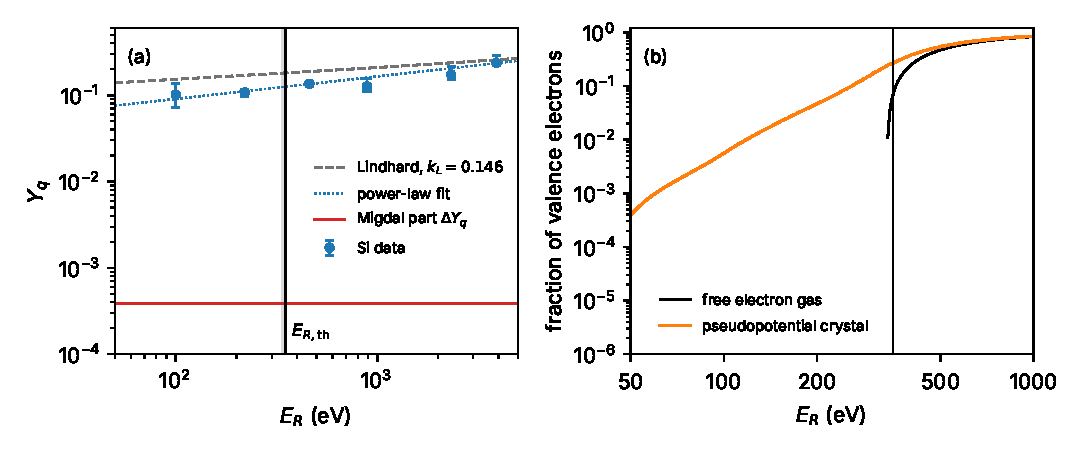
\includegraphics[width=\linewidth]{figures/ch19/fig19_2.pdf}
  \caption{The charge channel of silicon recoils. (a) Measured ionization yield $Y_q$ of silicon nuclear recoils (points: neutron scattering, total uncertainties, with \SI{3.8}{eV} per pair~\cite[Table~II]{albakry2023first}) against the recoil energy, with the power-law fit of the same work, $0.302(E_R/\SI{10}{keV})^{0.261}$ (dotted), and Lindhard's yield \cref{eq:16.6-lindhard} with $k_L = 0.146$ (dashed). Vertical line: the binary threshold $E_{R,\mathrm{th}} = \SI{352}{eV}$ of \cref{eq:19.2-Eth}; gray band: down to \SI{336}{eV}, the threshold with the $v_N^2$ term kept. Red: the part $\Delta Y_q^{\mathrm{Mig}}$ of the yield carried by Migdal electrons, \cref{eq:19.2-Ymig}, from the soft-limit spectrum of \cref{sec:12.3} converted to pairs by the silicon cascade of \cref{chap:18} with a uniform split of energy between electron and hole. (b) Fraction of valence electrons fast enough to be promoted across the gap $\Eg = \SI{1.17}{eV}$ by a head-on binary collision, $p \ge p_{\mathrm{min}}(E_R)$ of \cref{eq:19.2-pmin}: free electron gas of the valence density (black), which vanishes at \SI{336}{eV}, and the valence momentum density of the empirical pseudopotential model of \cref{sec:3.3} (four bands, $10^3$ points in the zone, plane waves to \SI{5.3}{\angstrom^{-1}}), whose smooth pseudo-orbitals understate the high-momentum tail; vertical line as in (a).}
  \label{fig:19-yield}
\end{figure}

\Cref{fig:19-yield}(a) shows the result. Between \SI{0.1}{keV} and \SI{3.9}{keV} the yield rises only from 0.10 to 0.24, and the two points below $E_{R,\mathrm{th}}$, at 0.10 and \SI{0.22}{keV}, agree with each other within their errors: there is no sign of an ionization threshold above \SI{100}{eV}. The Lindhard yield lies above the data at every energy below a keV, by a factor of 1.5 at \SI{100}{eV} (0.153 against 0.102) and by 1.4 at \SI{0.46}{keV}. Germanium, however, shows the opposite deviation. Recoils of \SI{254}{eV}, below its binary threshold of \SI{399}{eV}, give \SI{64 \pm 8}{eV} of electron-equivalent energy at \SI{77}{K}, a quenching factor of $\SI{25 \pm 3}{\percent}$ against Lindhard's \SI{14.3}{\percent}~\cite[abstract and Table~IV]{kavner2024measurement}.

The measured Fano factor of the nuclear-recoil charge, $F_{\mathrm{NR}} = \operatorname{Var}N_{\mathrm{eh}}/\langle N_{\mathrm{eh}}\rangle$, is $0.9^{+0.7}_{-0.4}$ at \SI{0.10}{keV}, $0.5^{+0.2}_{-0.1}$ at \SI{0.22}{keV} and $1.8^{+0.6}_{-0.5}$ at \SI{0.46}{keV}, and it grows to $8.4^{+2.4}_{-1.9}$ at \SI{3.91}{keV}~\cite[Table~II]{albakry2023first}, seventy times the electron-recoil value $F_{\mathrm{eh}} = 0.119$. Suppose the electronic energy $E_{\mathrm{el}}$ of a recoil were converted at a constant $\varepsilon_{\mathrm{eh}}$. The law of total variance would then give $\operatorname{Var}N_{\mathrm{eh}} = F_{\mathrm{eh}}\langle E_{\mathrm{el}}\rangle/\varepsilon_{\mathrm{eh}} + \operatorname{Var}E_{\mathrm{el}}/\varepsilon_{\mathrm{eh}}^2$, the cascade fluctuation at fixed $E_{\mathrm{el}}$ plus the fluctuation of $E_{\mathrm{el}}$ itself, so that
\begin{equation}
  F_{\mathrm{NR}} = F_{\mathrm{eh}} + \frac{\operatorname{Var}E_{\mathrm{el}}}{\varepsilon_{\mathrm{eh}}\langle E_{\mathrm{el}}\rangle} .
  \label{eq:19.2-FNR}
\end{equation}
At \SI{3.91}{keV}, with $\langle E_{\mathrm{el}}\rangle = Y_qE_R = \SI{923}{eV}$ and \SI{3.8}{eV} per pair, the measured $F_{\mathrm{NR}}$ requires a spread of \SI{170}{eV}, \SI{18}{\percent} of the mean: recoils of the same energy differ in how much of it reaches the electrons, because the sequence of collisions that each one makes is different. At \SI{100}{eV} the excitations lie near the gap and \cref{eq:19.2-FNR} no longer applies; there $F_{\mathrm{NR}}$ near one is what a few independent excitations of about one pair each would give.

\subsection{Migdal electrons in the measured yield}\label{sec:19.2-migdal}

The kick that starts the recoil already excites electrons, with the Migdal probability $P_{\mathrm{Mig}}$ of \cref{chap:12}. A neutron calibration measures the charge of real recoils, Migdal electrons included. The Migdal part of the yield is the integral \cref{eq:19.2-charge} taken over the soft-limit spectrum \cref{eq:12.3-soft}:
\begin{equation}
  \Delta Y_q^{\mathrm{Mig}} = \frac{\varepsilon_{\mathrm{eh}}}{E_R}\int\dd\omega_e\,\frac{\dd P_{\mathrm{Mig}}}{\dd\omega_e}\,\bar n(\omega_e) .
  \label{eq:19.2-Ymig}
\end{equation}
In the soft limit $\dd P_{\mathrm{Mig}}/\dd\omega_e$ is proportional to $v_N^2 = 2E_R/M_\kappa$, so the factor $1/E_R$ cancels and $\Delta Y_q^{\mathrm{Mig}}$ does not depend on the recoil energy. For silicon, the spectrum of \cref{sec:12.3} has $P_{\mathrm{Mig}} = 6.07\times10^{-3}$ at $E_R = \SI{100}{eV}$ with a mean electronic energy of \SI{5.97}{eV}. The energy-only cascade of \cref{chap:18} turns one such excitation into 1.69 pairs on average with a uniform split of the energy above the gap, or 1.92 if the electron takes all of it; the full-band cascade of \cref{sec:18.3-fullband} puts fewer events in the two-pair bin, and every Migdal excitation makes at least one pair. With \SI{3.8}{eV} per pair, the convention of the data,
\begin{equation*}
  \Delta Y_q^{\mathrm{Mig}} = \frac{\SI{3.8}{eV}}{\SI{100}{eV}}\times6.07\times10^{-3}\times1.69 = 3.9\times10^{-4} ,
\end{equation*}
and $4.4\times10^{-4}$ for the one-sided split; one pair per excitation gives the model-free lower edge $2.3\times10^{-4}$. The upper value is \SI{0.4}{\percent} of the measured yield at \SI{100}{eV} and \SI{0.3}{\percent} at \SI{0.46}{keV}. Both are soft-limit values, and the exact second-order bracket of \cref{sec:12.3-validity} lowers them, multiplying the Migdal probability by 0.93 at \SI{100}{eV} and by 0.62 at \SI{500}{eV}. The measured charge of silicon recoils at these energies is therefore almost entirely collisional.

A rate converted with the measured yield already contains the Migdal ionization (\cref{sec:12.1-counting}). Conversely, a computed yield must count the Migdal excitation at the kick and the collisional excitation after it, and nothing else. The trajectory calculation therefore starts after the kick, from the nuclear momentum and site distribution that the response hands over (\cref{sec:19.1}), and the lattice factor of the recoils that leave no Migdal electron has the weight $1 - P_{\mathrm{Mig}}$ of \cref{sec:12.1}, a \SI{0.6}{\percent} correction at \SI{100}{eV}. \Cref{sec:12.3-validity} met the boundary between the two channels from the Migdal side. Toward \SI{1}{keV} the second-order Migdal amplitude acquires a vanishing denominator, because the already moving nucleus ionizes the electrons on shell as a slow ion does, and that part belongs to the collisional channel of this section.

The balance between Migdal and collisional excitation shifts at low energy. The number of Migdal pairs per recoil falls in proportion to $E_R$. The collisional channel decreases for two reasons, fewer close collisions and the adiabatic suppression, whose factor $\ee^{-\xi_{\mathrm{M}}}$ falls from $1.1\times10^{-3}$ at \SI{100}{eV} to $2.6\times10^{-7}$ at \SI{20}{eV}, against a factor of five for the Migdal probability. If promotion at crossings follows the same trend, an estimate that only the kernel can confirm, the Migdal electrons become the dominant source of charge somewhere between a few tens of eV and \SI{100}{eV}, the recoil energies of dark matter below about \SI{0.44}{GeV}. That makes the Migdal rate of \cref{chap:12}, and not an extrapolated yield, the charge signal of the lightest nuclear-recoil searches.

\subsection{Open problems}\label{sec:19.2-open}

No calculation predicts the measured silicon yields and Fano factors below the binary threshold, or the germanium point at \SI{254}{eV}. The missing input is the close-collision kernel \cref{eq:19.2-kernel} for Si--Si and Ge--Ge collisions, with its exchange--correlation spread. Once it exists, the chain of partition trajectories, kernel and cascade also yields the probability of a recoil without charge, which sets the efficiency of a charge readout at the lowest recoil energies.

\section{Stopping of slow ions}\label{sec:19.3}

Nearly every nuclear-recoil search in a semiconductor converts measured charge into recoil energy with one formula, Lindhard's electronic share $y_L(E_R)$ of \cref{eq:16.6-lindhard}. For silicon it gives $y_L = 0.302$ at \SI{10}{keV}, and the measured yields of \cref{fig:19-yield} lie below it, by the factor 1.5 of \cref{sec:19.2-yield} at \SI{100}{eV}. The formula is the solution of an integral equation for an ion slowing down by independent binary collisions, with electronic losses taken from the stopping of a uniform electron gas. In the language of \cref{sec:19.1} it is the partition \cref{eq:19.1-partition} with $E_{\mathrm{st}} = 0$ and $\omega_e$ computed from continuum stopping. We will derive Lindhard's equation from that partition and see which of its assumptions fail below a keV. The Bethe formula, derived from the loss function of \cref{sec:4.4}, then gives the opposite, first-order limit: there the solid enters through one mean excitation energy, and the limit sets in only above about twice the Fermi velocity, far above any recoil.

Two objects carry Lindhard's name. The Lindhard function $\varepsilon_{\mathrm{Lin}}$ of \cref{sec:4.5} is the dielectric function of the free electron gas; Lindhard quenching is the electronic share $y_L$ of a slowing-down ion. Their only connection is that the electronic stopping behind $y_L$ was first estimated from an electron gas.

\subsection{Binary collisions of a slow ion}\label{sec:19.3-binary}

A silicon recoil of \SI{1}{keV} moves at $v_N = 2.76\times10^{-4}$, a twenty-fifth of the Fermi velocity of the valence electrons (\cref{we:19-threshold}). It loses energy in two ways, which Lindhard's model treats as separate: elastic collisions with other nuclei, screened by their electrons, and excitation of the electrons themselves.

The nuclear collisions are those of two atoms interacting through a screened Coulomb potential $(Z_\kappa^2\alpha/r)\,\phi_{\mathrm{TF}}(r/a_L)$, with $\phi_{\mathrm{TF}}$ the Thomas--Fermi screening function of a neutral atom~\cite{thomas1927calculation,fermi1928statistische} and $a_L = 0.8853\,a_0/(\sqrt2\,Z_\kappa^{1/3})$ Lindhard's screening length for two equal atoms~\cite[Sect.~II\,A]{sorensen2015atomic}. For silicon, $a_L = \SI{0.1375}{\angstrom}$. The natural energy scale is the Coulomb energy of the pair at the distance $a_L$. For equal masses the center-of-mass frame carries half of the ion's kinetic energy $E$, and the reduced energy is
\begin{equation}
  \epsilon_L = \frac{a_L}{2Z_\kappa^2e_{\mathrm{G}}^2}\,E \equiv c_L E ,
  \label{eq:19.3-reduced}
\end{equation}
with $e_{\mathrm{G}}^2 = \alpha$ the Gaussian charge squared, \SI{14.40}{eV\,\angstrom} in conventional units. For silicon $c_L = \SI{0.02435}{keV^{-1}}$, the value $11.5\,Z_\kappa^{-7/3}\,\si{keV^{-1}}$ of \cref{eq:16.6-lindhard}: a recoil of \SI{1}{keV} has $\epsilon_L = 0.024$, and $\epsilon_L = 1$ is reached only at \SI{41}{keV}.

A collision that deflects the pair by the angle $\theta_{\mathrm{s}}$ in the center-of-mass frame gives the struck atom the energy $T_n = E\sin^2(\theta_{\mathrm{s}}/2)$. Lindhard's insight was that in the reduced variable $x_L = \epsilon_L\sin(\theta_{\mathrm{s}}/2)$ the cross-section of a screened Coulomb potential depends on one function of one variable,
\begin{equation}
  \dd\sigma_n = \pi a_L^2\,\frac{f_{\mathrm{LSS}}(x_L)}{x_L^2}\,\dd x_L ,
  \label{eq:19.3-dsigma}
\end{equation}
with $t = x_L^2$ the form of~\cite[Eq.~(2)]{sarkis2023ionization}. The reason is visible in the small-angle (impulse) approximation, where the deflection is the transverse momentum the potential imparts along a straight path divided by the momentum. With $\beta = b/a_L$ the impact parameter in units of $a_L$ and $I(\beta) = \int_0^\infty\dd\zeta\,\phi_{\mathrm{TF}}(r)/r$, $r = (\beta^2 + \zeta^2)^{1/2}$, the deflection is $\theta_{\mathrm{s}} = -\epsilon_L^{-1}\,\dd I/\dd\beta$, so that $x_L \simeq \epsilon_L\theta_{\mathrm{s}}/2 = -\tfrac12\,\dd I/\dd\beta$ is a function of $\beta$ alone. Then $\dd\sigma_n = 2\pi a_L^2\beta\,\dd\beta$ gives $f_{\mathrm{LSS}}(x_L) = 2x_L^2\beta\,|\dd\beta/\dd x_L|$, with no reference to the energy. An unscreened potential, $\phi_{\mathrm{TF}} = 1$, has $\dd I/\dd\beta = -1/\beta$ and gives the Rutherford form $f_{\mathrm{LSS}} = 1/2x_L$. The screened function rises as a power of $x_L$ at small $x_L$, peaks at 0.43 near $x_L = 0.14$ and approaches the Rutherford form for $x_L \gg 1$. The mean energy lost to nuclei per unit reduced path, $s_n(\epsilon_L) = \epsilon_L^{-1}\int_0^{\epsilon_L}f_{\mathrm{LSS}}\,\dd x_L$, peaks at 0.41 near $\epsilon_L = 0.3$.

The electronic losses are a friction. For a projectile much slower than the electrons, the dielectric stopping \cref{eq:4.4-dEdx} samples only the low-energy side of the loss function, and the energy loss per unit path is proportional to $v_N$. \Cref{we:4-oscillatorL} showed this for a damped oscillator, and \cref{lim:19.3b} below shows it for the electron gas. Since $E \propto v_N^2$, the reduced electronic stopping per unit reduced path length $\rho_L = \pi a_L^2\nd_{\mathrm{at}}x$, with $x$ the path length and $\nd_{\mathrm{at}}$ the atomic density, is
\begin{equation}
  \frac{\dd\epsilon_L}{\dd\rho_L}\bigg|_e = k_L\,\epsilon_L^{1/2} , \qquad k_L = 0.133\,Z_\kappa^{2/3}A^{-1/2} ,
  \label{eq:19.3-Se}
\end{equation}
with $A$ the atomic mass in atomic units~\cite[Eq.~(4)]{sarkis2020study}. For silicon $k_L = 0.146$. The coefficient comes from Lindhard and Scharff's estimate of the friction of an ion in an electron gas. It contains a factor of about $Z_\kappa^{1/6}$, 1.55 for silicon, inserted by hand to match the stopping data of their time, as Sarkis et al.\ point out~\cite[Sect.~``Scaling length'']{sarkis2023ionization}. In physical units \cref{eq:19.3-Se} assigns a silicon ion in silicon an electronic stopping of 0.88, 2.77 and \SI{8.76}{eV/\angstrom} at 0.1, 1 and \SI{10}{keV}.

The friction law is an empirical scaling at these speeds, not a derived limit. The dielectric formula \cref{eq:4.4-dEdx} is first order in the ion's charge, and its expansion parameter for a silicon ion among the valence electrons is the Born parameter $Z_\kappa\alpha/v_{\mathrm{F}} = 14.6$ (\cref{sec:19.2-kernel}). Taken at face value, the electron gas of the valence density gives a proton at the speed of a \SI{1}{keV} silicon recoil a stopping of \SI{0.32}{eV/\angstrom}. The first-order stopping of the silicon ion would be $Z_\kappa^2 = 196$ times that, \SI{64}{eV/\angstrom}, which is 23 times the value of \cref{eq:19.3-Se}. The ion's own electrons screen its charge, and the slow collision is far from linear response. \Cref{eq:19.3-Se} keeps only the scaling with $v_N$ and fits the coefficient.

\subsection{Lindhard's integral equation}\label{sec:19.3-integral}

Follow the ion of \cref{sec:19.1} as a sequence of collisions. Each collision transfers $T_n$ to a target atom, which starts its own slowing-down, and energies $T_{e,i}$ to electrons. Let $T_{\mathrm{d}}(E)$ be the mean energy that an ion starting with kinetic energy $E$ eventually gives to atomic motion, summed over itself and all the atoms it sets moving: the damage energy of \cref{eq:16.6-lindhard}, as a function of the starting energy. The electronic share is the rest, $E - T_{\mathrm{d}}(E)$. In the partition \cref{eq:19.1-partition} at $E_{\mathrm{st}} = 0$, $T_{\mathrm{d}}$ is the part of $E_{\mathrm{lat}}$ delivered by nuclear collisions and $E - T_{\mathrm{d}}$ is $\omega_e$; the phonons that the electrons later emit in their cascade belong to $E_{\mathrm{heat}}$ but not to $T_{\mathrm{d}}$.

Two assumptions turn this into an equation. The first is that collisions are binary, with targets at rest and uncorrelated with each other, so that the struck atom starts an independent copy of the same process. The second is that the ion has no memory, so that after a collision it is again an ion of the new energy in a fresh medium. Then the mean damage energy before a collision equals the sum of the mean damage energies of the three objects after it. These are the scattered ion with energy $E - T_n - \sum_iT_{e,i}$, the struck atom with $T_n - U$, where $U$ is the energy spent breaking its binding, and the excited electrons. Averaging over all collisions, which is the integral over the cross-section,
\begin{equation}
  \int\dd\sigma_{n,e}\,\Bigl[T_{\mathrm{d}}\Bigl(E - T_n - \sum_iT_{e,i}\Bigr) + T_{\mathrm{d}}(T_n - U) - T_{\mathrm{d}}(E) + \sum_iT_{\mathrm{d}}^{(e)}(T_{e,i})\Bigr] = 0 ,
  \label{eq:19.3-basic}
\end{equation}
which is Lindhard's basic integral equation~\cite{lindhard1963integral}, as quoted by Sarkis et al.~\cite[Eq.~(3)]{sarkis2020study}, with $T_{\mathrm{d}}^{(e)}$ the damage energy an excited electron produces. The equation holds for the mean of any quantity that adds up over the collisions; the damage energy is one such quantity. It is the first-moment equation of a branching process, the nuclear counterpart of the cascade of \cref{sec:18.1}.

Lindhard reduced \cref{eq:19.3-basic} with five further approximations, as quoted by Sarkis et al.~\cite[Sect.~II]{sarkis2020study}: (A) excited electrons give no appreciable energy back to atoms, so the last term is dropped; (B) the binding $U$ is set to zero; (C) the energy given to electrons in one collision is small compared to $E$; (D) nuclear and electronic collisions are separate events; (E) the nuclear transfer $T_n$ is small compared to $E$ where it matters for the electronic term. With (C) the first term is expanded to first order in the electronic transfer,
\begin{equation*}
  T_{\mathrm{d}}\Bigl(E - T_n - \sum_iT_{e,i}\Bigr) \simeq T_{\mathrm{d}}(E - T_n) - T_{\mathrm{d}}'(E)\sum_iT_{e,i} ,
\end{equation*}
where (E) puts the derivative at $E$ rather than at $E - T_n$. By (D) each collision is either nuclear, with $T_{e,i} = 0$, or electronic, with $T_n = 0$. The electronic collisions then contribute $-T_{\mathrm{d}}'(E)\int\dd\sigma_e\sum_iT_{e,i}$, and the integral is the electronic stopping per atom, $(\dd E/\dd x)_e/\nd_{\mathrm{at}}$. The nuclear collisions contribute the bracket with $\sum_iT_{e,i} = 0$ and $U = 0$, integrated with \cref{eq:19.3-dsigma}. In reduced units, $\epsilon_{\mathrm{d}} = c_LT_{\mathrm{d}}$, with \cref{eq:19.3-Se} for the stopping and $T_n/E = x_L^2/\epsilon_L^2$,
\begin{equation}
  k_L\,\epsilon_L^{1/2}\,\epsilon_{\mathrm{d}}'(\epsilon_L) = \int_0^{\epsilon_L}\dd x_L\,\frac{f_{\mathrm{LSS}}(x_L)}{x_L^2}\Bigl[\epsilon_{\mathrm{d}}\Bigl(\epsilon_L - \frac{x_L^2}{\epsilon_L}\Bigr) + \epsilon_{\mathrm{d}}\Bigl(\frac{x_L^2}{\epsilon_L}\Bigr) - \epsilon_{\mathrm{d}}(\epsilon_L)\Bigr] ,
  \label{eq:19.3-simple}
\end{equation}
Lindhard's simplified equation~\cite[Eq.~(5)]{sarkis2020study}, with $\epsilon_{\mathrm{d}} \to \epsilon_L$ as $\epsilon_L \to 0$. The left side is the energy the ion would have delivered to atoms but gave to electrons along a unit of reduced path; the right side is what the nuclear collisions along the same path redistribute between the ion and the atoms it strikes. The upper limit $x_L = \epsilon_L$ is the head-on collision, which hands the whole energy to the struck atom.

The small-energy behavior shows where the formula's shape comes from. Continue the screened cross-section below the tabulated range as Lindhard's power law $f_{\mathrm{LSS}} = \lambda_Lx_L^{1/3}$ and try $\epsilon_{\mathrm{d}} = \epsilon_L - C\epsilon_L^p$ and keep the first order in $k_L$. The leading term $\epsilon_L$ makes the bracket vanish identically, since the energies of ion and target add up to $\epsilon_L$. With $x_L^2/\epsilon_L = \epsilon_Ls$ the right side becomes $\tfrac12\lambda_LC\,\epsilon_L^{p - 2/3}J$, with $J = \int_0^1\dd s\,s^{-4/3}[1 - (1 - s)^p - s^p]$, and the left side is $k_L\epsilon_L^{1/2}$ to this order. Matching the powers gives $p = 7/6$ and $C = 2k_L/(\lambda_LJ)$:
\begin{equation}
  y_L = 1 - \frac{\epsilon_{\mathrm{d}}}{\epsilon_L} \simeq \frac{2k_L}{\lambda_LJ}\,\epsilon_L^{1/6} , \qquad J = 0.4742 .
  \label{eq:19.3-asym}
\end{equation}
With the screened cross-section used below, $\lambda_L = 1.283$ and the coefficient is $3.29\,k_L$. This is the origin of the leading term $3\epsilon_L^{0.15}$ of $g_L$ in \cref{eq:16.6-lindhard}. With this continuation the electronic share falls as the sixth root of the energy, because a slow ion keeps handing its energy on to slower atoms, each of which loses a fraction to electrons. The law is a property of the assumed $x_L^{1/3}$ continuation, not of the screened Coulomb potential: the Thomas--Fermi screening function falls as $r^{-3}$, the potential as $r^{-4}$, and $f_{\mathrm{LSS}} \propto x_L^{1/2}$ at the smallest $x_L$. With that tail the nuclear and electronic stopping scale alike and $y_L$ tends to a nonzero constant as $\epsilon_L \to 0$.

\Cref{eq:19.3-simple} has no closed solution for a screened potential. Lindhard and coworkers solved it numerically, and the parametrization of \cref{eq:16.6-lindhard}, $y_L = k_Lg_L/(1 + k_Lg_L)$ with $g_L = 3\epsilon_L^{0.15} + 0.7\epsilon_L^{0.6} + \epsilon_L$, is Lewin and Smith's fit to their solution~\cite{lewin1996review}, as quoted by Sorensen~\cite[Eqs.~(5)--(7)]{sorensen2015atomic}. We solve the equation again to see how well the fit represents it. The cross-section is built as above, from the Thomas--Fermi function solved numerically ($\phi_{\mathrm{TF}}'(0) = -1.58807$) and the impulse deflection, and continued below $x_L = 2\times10^{-3}$, where Lindhard did not tabulate $f_{\mathrm{LSS}}$~\cite[Sect.~II\,D]{sorensen2015atomic}, by the power law $\lambda_Lx_L^{1/3}$. The equation involves $\epsilon_{\mathrm{d}}$ only at energies up to $\epsilon_L$, so it can be integrated upward from the asymptotic form \cref{eq:19.3-asym}; the right end of the integral, which involves $\epsilon_{\mathrm{d}}'(\epsilon_L)$ itself, is solved exactly at each step. Halving both grids changes $y_L$ by less than $5\times10^{-4}$.

\begin{limitbox}[Lindhard quenching][lim:19.3a]
Lindhard's electronic share of a recoil in a one-element target~\cite{lindhard1963integral}, \cite[Eq.~(3)]{agnese2018nuclear}, \cref{eq:16.6-lindhard}: $y_L = k_Lg_L(\epsilon_L)/[1 + k_Lg_L(\epsilon_L)]$, $g_L = 3\epsilon_L^{0.15} + 0.7\epsilon_L^{0.6} + \epsilon_L$, with $k_L$ and $\epsilon_L$ of \cref{eq:19.3-Se,eq:19.3-reduced}.
\par\smallskip
{\centering
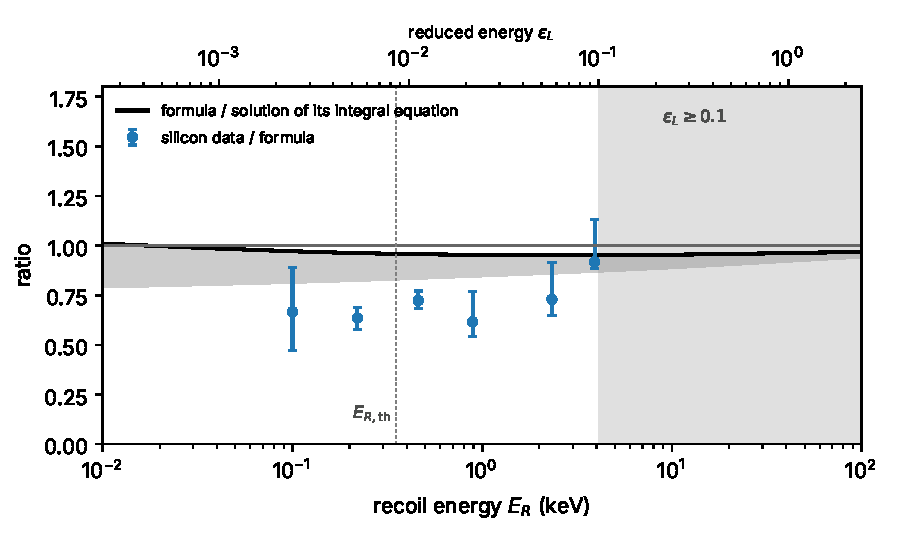
\includegraphics[width=\linewidth]{figures/ch19/limit19_3a.pdf}
\captionof{figure}{Silicon, $k_L = 0.146$, against the recoil energy. Solid: the formula divided by the numerical solution of the binary-collision equation \cref{eq:19.3-simple} with the Thomas--Fermi cross-section in the impulse approximation, continued below $x_L = 2\times10^{-3}$ as $x_L^{1/3}$; dark band: the same with continuation exponents from 1/3 to the local slope 0.363 of the computed cross-section, a sensitivity to that choice. Points: the measured silicon yields~\cite[Table~II]{albakry2023first} divided by the formula. Dashed: the constant-binding model with $U = \SI{0.15}{keV}$~\cite[Eq.~(13), Table~3]{sarkis2020study} divided by the formula. Gray: $\epsilon_L \ge 0.1$, $E_R \ge \SI{4.1}{keV}$, where the formula describes the silicon data~\cite[Sect.~II]{sarkis2020study}. Vertical line: the binary threshold $E_{R,\mathrm{th}} = \SI{352}{eV}$.}\label{fig:19-limit-lindhard}
\par}
\smallskip
Below a few keV the measured yields fall 8 to \SI{38}{\percent} under the formula, a deficit comparable to the formula's sensitivity to its softest collisions; the stored energy, the gap and the conversion to pairs that the model omits also act there.
\end{limitbox}

With the $x_L^{1/3}$ continuation the solution and the fit agree to \SI{3}{\percent} below \SI{100}{eV}, and the fit lies \SIrange{4}{5}{\percent} below the solution between 1 and \SI{20}{keV}, where $y_L$ is 0.210 against 0.220 at \SI{1}{keV}. The continuation matters more than the fit. Continuing the computed cross-section at its own local slope, 0.363 at $x_L = 2\times10^{-3}$, raises the solution by \SI{13}{\percent} at \SI{1}{keV} and by \SI{10}{\percent} at \SI{4}{keV}; an exponent of 0.30 lowers it by \SI{11}{\percent} at \SI{1}{keV}, and 0.40 raises it by \SI{40}{\percent}. The dark band of \cref{fig:19-limit-lindhard} is therefore a sensitivity to one modeling choice, not an uncertainty. Nothing places the true yield between the two continuations: below the matching point the Thomas--Fermi cross-section steepens toward $x_L^{1/2}$, while binding and the lattice remove the softest transfers altogether. Below $\epsilon_L = 2\times10^{-3}$, about \SI{80}{eV}, the whole cross-section of a slow secondary lies in the continued region, and the binary model does not determine the yield of a keV recoil there. Those are the soft collisions of the slowest secondaries, at energies of tens of eV, where atoms are bound and the binary model has least claim to hold. The equation propagates their treatment upward because every recoil ends as a population of such secondaries.

\subsection{Implicit assumptions of Lindhard quenching}\label{sec:19.3-assumptions}

Read against the partition of \cref{sec:19.1}, the chain from \cref{eq:19.3-basic} to $y_L$ makes three assumptions that its list of approximations does not name: no stored energy, electronic friction down to zero speed, and conversion to pairs in proportion. Each fails below a keV in silicon.

The first is that no energy is stored. With $U = 0$ every collision returns its full transfer to atomic motion, and an atom that ends displaced keeps no energy in the lattice: $E_{\mathrm{st}} = 0$ in \cref{eq:19.1-partition}. Restoring $U$ does not repair this. In the constant-binding model of Sarkis et al.~\cite[Eqs.~(9), (13)]{sarkis2020study} the struck atom pays $U$ before it moves, the lower limit of the integral in \cref{eq:19.3-simple} becomes $(\epsilon_Lc_LU)^{1/2}$, and the yield vanishes near $E_R = 2U$. Their fit to the silicon data above \SI{0.68}{keV} gives $U = 0.15 \pm \SI{0.06}{keV}$~\cite[Table~3]{sarkis2020study}, and with the fitted correction terms the yield reaches zero at \SI{298}{eV} (\cref{fig:19-yields}); the measured yield at \SI{100}{eV} is $0.102^{+0.034}_{-0.030}$. The later model of the same authors replaces $U$ by a function $U(E) = U_{\mathrm{FP}} + U_{\mathrm{EDFT}}(E)$: a constant $U_{\mathrm{FP}} = \SI{23.6}{eV}$, which the authors call the Frenkel-pair creation energy and take from averaged displacement thresholds, plus an energy-dependent excitation of the inner electrons. It adds electronic straggling and a modern stopping model, and it fits 102 points from \SI{0.68}{keV} to \SI{3}{MeV} with $\chi^2/\mathrm{dof} = 1870/101$; its threshold lies just above $U_{\mathrm{FP}}$~\cite[Eqs.~(2)--(4), Fig.~3]{sarkis2023ionization}. The configurational energy of a Frenkel pair in silicon is 6.8 to \SI{9.7}{eV} (\cref{sec:7.4}), a third of $U_{\mathrm{FP}}$; in the partition that part is stored energy and the rest of a threshold-sized $U_{\mathrm{FP}}$ is heat. In both models, however, the $U$ spent by secondary atoms appears as an argument of $T_{\mathrm{d}}(T_n - U)$, is missing from the damage energy, and therefore lands in the electronic share $E - T_{\mathrm{d}}$ by complement. Energy that the partition stores in defects is counted as ionization.

The second is that electronic losses follow the friction law down to zero speed. \Cref{eq:19.3-Se} gives a silicon ion of \SI{100}{eV} an electronic stopping of \SI{0.88}{eV/\angstrom}, while a binary collision at that energy cannot create a pair at all (\cref{sec:19.2-binary}), and the momentum tail lets through a fraction $5.6\times10^{-3}$ of the valence electrons (\cref{sec:19.2-soft}). Below $E_{R,\mathrm{th}}$ the friction assigns losses to final states that are strongly suppressed. The modified equation of Sarkis et al.\ also keeps a term $-\tfrac12k_L\epsilon_L^{3/2}\epsilon_{\mathrm{d}}''$, obtained from the second-order expansion with the mean nuclear transfer $\epsilon_L/2$ in a collision that also excites electrons~\cite[Eq.~(9), App.~B]{sarkis2020study}. Under approximation (D) every collision has $T_n = 0$ or $\sum_iT_{e,i} = 0$, so the cross term $T_n\sum_iT_{e,i}$ that produces it vanishes identically, and the term contradicts the separation used to obtain the stopping.

The third is that the electronic share becomes charge in proportion, $N_{\mathrm{eh}} = y_LE_R/\varepsilon_{\mathrm{eh}}$, with every pair collected and none trapped. Then $Y_q = y_L$. The excitations of a slow ion lie near the gap, where the cascade gives one pair per excitation rather than $\omega_e/\varepsilon_{\mathrm{eh}}$ (\cref{eq:19.2-charge}), so $y_L$ and $Y_q$ differ even if $y_L$ were exact. Trapping and incomplete collection lower the measured charge further (\cref{sec:18.5,sec:19.5}).

The approximations that the list does name are weakest at the same energies. The medium is a random gas of atoms, with no channels and no dependence on direction, and collisions are binary and independent, which fails in the dense cascades of germanium recoils of a few keV. The reduced energy is also convention-dependent. Sarkis et al.\ define it in their later work with the universal screening length and an effective projectile charge $Z_1 = 12$. This maps the same recoil energy to a reduced energy \SI{10}{\percent} higher than \cref{eq:19.3-reduced}~\cite[Sect.~``The nuclear recoil QF'']{sarkis2023ionization}, so that fitted constants cannot be carried from one convention to the other.

\begin{figure}[tbp]
  \centering
  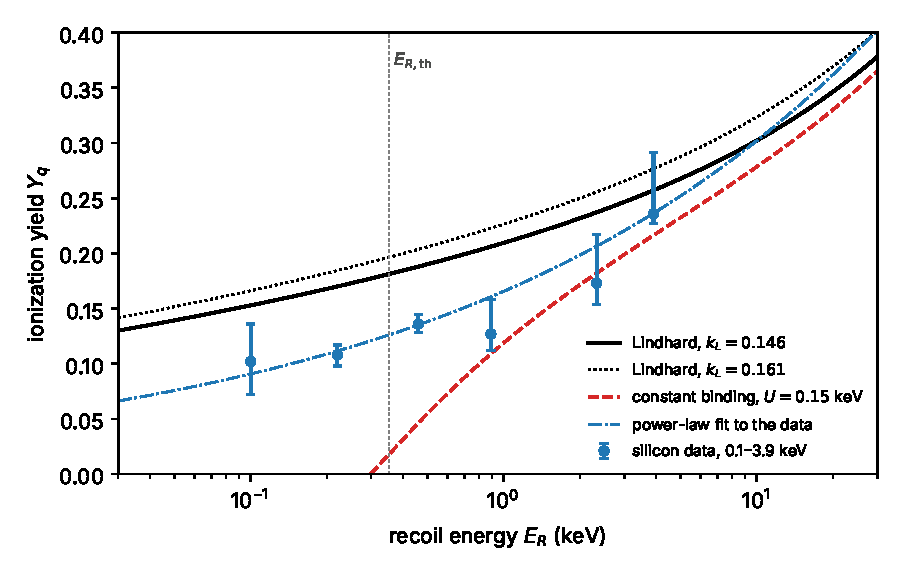
\includegraphics[width=\linewidth]{figures/ch19/fig19_3.pdf}
  \caption{Lindhard and modified-Lindhard yields of silicon against the measured ionization yield. Solid: Lindhard's formula \cref{eq:16.6-lindhard} with $k_L = 0.146$; dotted: with $k_L = 0.161$, the value of a fit of the numerical constant-binding solution to the silicon data~\cite[Table~4]{sarkis2020study}. Dashed: the constant-binding model of Sarkis et al.\ with $U = \SI{0.15}{keV}$, $C_0 = 9.1\times10^{-3}$ and $C_1 = 3.33\times10^{-5}$~\cite[Eq.~(13), Table~3]{sarkis2020study}, which vanishes at \SI{298}{eV}. Points: the silicon measurement with total uncertainties~\cite[Table~II]{albakry2023first}; dash-dotted: its power-law fit $0.302(E_R/\SI{10}{keV})^{0.261}$, pinned to the formula at \SI{10}{keV}. Vertical line: the binary threshold $E_{R,\mathrm{th}} = \SI{352}{eV}$ (\cref{sec:19.2}).}
  \label{fig:19-yields}
\end{figure}

\Cref{fig:19-yields} shows the result of these assumptions. Raising $k_L$ moves the whole curve up and away from the sub-keV data. Adding a constant binding brings the curve down to the data near \SI{2}{keV} only by introducing a cutoff that the data at 0.10 and \SI{0.22}{keV} contradict. The data themselves follow the power law $E_R^{0.26}$ from \SI{0.1}{keV} to \SI{3.9}{keV}, flatter than $y_L$ and with no threshold. Each modified model fixes one assumption and lets its fitted constants absorb the rest; a good fit therefore does not tell us which assumption was wrong. The calculation that would show it is the partition of \cref{sec:19.1} with stored energy, the excitation kernel of \cref{sec:19.2} and the cascade conversion, specified in \cref{app:E.23}. Above about \SI{4}{keV}, where stored energy and the gap are small fractions of the electronic share, Lindhard's formula describes the silicon data and needs no repair.

\subsection{Bethe stopping from the loss function}\label{sec:19.3-bethe}

At the opposite end of the speed range the stopping of an ion is a derived result. Take the dielectric stopping \cref{eq:4.4-dEdx} of a heavy projectile of charge $Z_1e$ and speed $v$ at $T = 0$, and suppose $v$ is large compared to the speeds of the electrons that hold the weight of the loss function. Split the momentum integral at a value $q_0$ chosen so that two conditions hold together: $q_0v$ lies far above the energies where $L$ has its weight, and $q_0$ is small compared to the inverse size of the atoms, so that $L(q,\omega) \simeq L(0,\omega)$ for $q < q_0$. Both are possible only if $v$ is large.

Below $q_0$ the loss function is its optical limit, and the condition $\omega \le qv$ becomes $q \ge \omega/v$. Exchanging the order of integration,
\begin{equation*}
  \int_0^{q_0}\frac{\dd q}{q}\int_0^{qv}\dd\omega\,\omega L(0,\omega) = \int_0^\infty\dd\omega\,\omega L(0,\omega)\,\ln\frac{q_0v}{\omega} ,
\end{equation*}
where the upper limit of the $\omega$ integral moved to infinity because $q_0v$ lies above the whole spectrum. Above $q_0$ the line $\omega = qv$ lies above the spectrum at every $q$ until it meets the free-electron recoil $\omega = q^2/2m_e$, at $q = 2m_ev$. Between $q_0$ and $2m_ev$ the inner integral is therefore the whole f-sum $(\pi/2)\omega_p^2$ of \cref{eq:4.4-fsumL}, and beyond $2m_ev$ it is zero, since the Bethe ridge has moved out of reach. The second piece is $(\pi/2)\omega_p^2\ln(2m_ev/q_0)$. Writing the f-sum as $\int_0^\infty\dd\omega\,\omega L(0,\omega) = (\pi/2)\omega_p^2$ in the first piece, $q_0$ cancels between the two, and with $\omega_p^2 = 4\pi\alpha\nd_e/m_e$ the prefactor $2Z_1^2\alpha/\pi v^2$ of \cref{eq:4.4-dEdx} times the f-sum $(\pi/2)\omega_p^2$ equals $4\pi Z_1^2\alpha^2\nd_e/(m_ev^2)$.

\begin{keyresult}[Bethe stopping from the loss function]
For a heavy projectile of charge $Z_1e$ and speed $v$ well above the speeds of the electrons that hold the weight of the loss function, in first order in $Z_1$,
\begin{equation}
  -\frac{\dd E}{\dd x} = \frac{4\pi Z_1^2\alpha^2\nd_e}{m_ev^2}\,\ln\frac{2m_ev^2}{\bar I} ,
  \label{eq:19.3-bethe}
\end{equation}
with the mean excitation energy defined by the logarithmic moment of the optical loss function,
\begin{equation}
  \ln\bar I = \frac{2}{\pi\omega_p^2}\int_0^\infty\dd\omega\;\omega\,L(0,\omega)\,\ln\omega ,
  \label{eq:19.3-lnI}
\end{equation}
where $\nd_e$ and $\omega_p$ count all the electrons of the target.
\end{keyresult}

\noindent This is the nonrelativistic limit of the Bethe equation of the Particle Data Group. Its bracket $\tfrac12\ln(2m_e\beta^2\gamma^2W_{\mathrm{max}}/I^2) - \beta^2$, with $W_{\mathrm{max}} = 2m_e\beta^2\gamma^2$ for a heavy projectile, becomes $\ln(2m_ev^2/I)$ up to terms of order $v^4$, and its prefactor $Kz^2(Z/A)/\beta^2$ per unit mass is $4\pi\alpha^2\nd_e/(m_ev^2)$ per unit length~\cite[Eq.~(34.5)]{navas2024review}. The Particle Data Group describes $I$ as a geometric average of the excitation energies weighted by their oscillator strengths~\cite[Sect.~34.2.1]{navas2024review}; \cref{eq:19.3-lnI} makes the weight precise for a condensed medium. It is the loss function, not $\varepsilon_2$, because the projectile couples to the total potential, and the logarithm sits inside the f-sum weight $\omega L$. The prefactor of \cref{eq:19.3-bethe} depends on the electron density alone, as \cref{sec:4.4} anticipated; the solid enters only through $\bar I$, and only logarithmically.

\begin{workedexample}{The mean excitation energy of silicon}\label{we:19-lnI}
Start with the four valence electrons in the single damped oscillator of \cref{we:4-oscillatorL} at $q \to 0$: $L(0,\omega) = \omega_p^2\varGamma_{\mathrm{w}}\omega/[(\omega^2 - \bar E^2)^2 + \varGamma_{\mathrm{w}}^2\omega^2]$ with $\omega_p = \SI{16.6}{eV}$, $\bar E = \SI{17.4}{eV}$ and $\varGamma_{\mathrm{w}} = \SI{3.66}{eV}$. For a narrow line \cref{eq:19.3-lnI} would give $\bar I = \bar E$, since all the weight sits at one energy. The damping spreads it: the model puts \SI{88}{\percent} of its f-sum between 10 and \SI{30}{eV}, but \SI{7.8}{\percent} between 30 and \SI{100}{eV} and \SI{2.4}{\percent} above, in a tail $\omega L \propto \varGamma_{\mathrm{w}}\omega_p^2/\omega^2$ that the logarithm weights heavily. Numerically,
\begin{equation*}
  \ln\bar I_{\mathrm{val}} = \frac{2}{\pi\omega_p^2}\int_0^\infty\dd\omega\,\omega L(0,\omega)\ln\frac{\omega}{\SI{1}{eV}} = 3.012 , \qquad \bar I_{\mathrm{val}} = \SI{20.3}{eV} ,
\end{equation*}
\SI{17}{\percent} above $\bar E$; a damping of \SI{2}{eV} brings it to \SI{19.0}{eV}. The inverse moment of \cref{eq:4.4-inverse} fixed $\bar E$ from the low-energy side of the spectrum; $\bar I$ is set by the high-energy side, and the two mean energies agree only for a narrow line.

The valence electrons are four of fourteen, and the core changes the answer by an order of magnitude. Take the measured loss function of \cref{sec:10.7}, which extends to \SI{30}{keV}. For all fourteen electrons $\omega_p = \SI{31.05}{eV}$ and $(\pi/2)\omega_p^2 = \SI{1514}{eV^2}$; the tabulated spectrum holds \SI{1537}{eV^2}, \SI{1.5}{\percent} more. Split at \SI{90}{eV}, below the L edge, and at \SI{1.83}{keV}, below the K edge, the f-sum weight $w_j$ and the logarithmic mean energy $\omega_j$ of each band are
\begin{equation*}
  \text{valence: } 0.280,\ \SI{19.5}{eV} ; \qquad \text{L shell: } 0.607,\ \SI{246}{eV} ; \qquad \text{K shell: } 0.113,\ \SI{3.17}{keV} ,
\end{equation*}
so that, with the spectrum normalized to its own f-sum, $\ln(\bar I/\SI{1}{eV}) = \sum_jw_j\ln(\omega_j/\SI{1}{eV}) = 0.832 + 3.340 + 0.910 = 5.082$ and $\bar I = \SI{161}{eV}$. Rescaling the spectrum to the exact f-sum leaves this value unchanged. It lies \SI{7}{\percent} below the adopted \SI{173.0}{eV} of the Particle Data Group~\cite{pdg2024atomic}, and the \SI{1.5}{\percent} excess of the tabulated f-sum is a measure of the error of the data. The L shell holds \SI{61}{\percent} of the oscillator strength and the valence electrons, which set every dark-matter rate of \cref{chap:10}, \SI{28}{\percent}; without the core shells $\bar I$ would be the \SI{19.5}{eV} of the valence band.
\end{workedexample}

The derivation needs two conditions, and both fail for recoils. The split at $q_0$ requires $2m_ev^2 \gg \bar I$, so that the logarithm is large: a proton of \SI{1}{MeV} has $2m_ev^2 = \SI{2.2}{keV}$, thirteen times the $\bar I$ of silicon, while a silicon recoil of \SI{10}{keV} has \SI{0.78}{eV}, $4.5\times10^{-3}$ of it, and \cref{eq:19.3-bethe} would give a negative stopping. The first-order treatment requires $Z_1\alpha/v \ll 1$: 0.16 for the proton, 117 for the recoil. \Cref{lim:19.3b} shows the first condition in an electron gas, where both formulas can be evaluated exactly.

\begin{limitbox}[Bethe stopping][lim:19.3b]
The Bethe formula in its nonrelativistic limit~\cite[Eq.~(34.5)]{navas2024review}, \cref{eq:19.3-bethe}: $-\dd E/\dd x = (4\pi Z_1^2\alpha^2\nd_e/m_ev^2)\ln(2m_ev^2/\bar I)$, with $\bar I$ from \cref{eq:19.3-lnI}.
\par\smallskip
{\centering
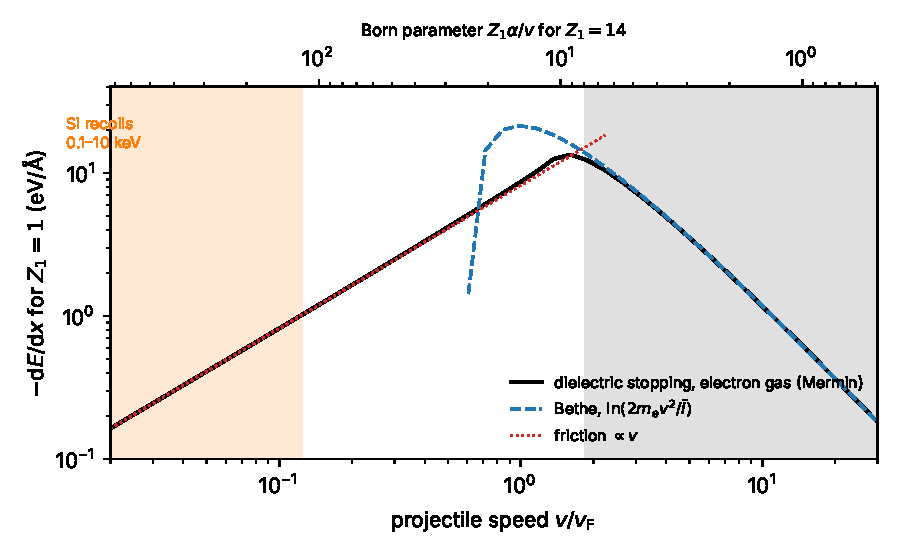
\includegraphics[width=\linewidth]{figures/ch19/limit19_3b.pdf}
\captionof{figure}{Stopping of a heavy projectile with $Z_1 = 1$ in the electron gas of the silicon valence density ($k_{\mathrm{F}} = \SI{1.8085}{\angstrom^{-1}}$, $v_{\mathrm{F}} = 6.98\times10^{-3}$, $\omega_p = \SI{16.6}{eV}$), against its speed. Solid: the dielectric stopping \cref{eq:4.4-dEdx} with the Mermin dielectric function of \cref{sec:4.5} and relaxation rate $0.1\,\omega_p$, a modeling choice that keeps the f-sum. Dashed: \cref{eq:19.3-bethe} with the model's own $\bar I = \SI{17.9}{eV}$ from \cref{eq:19.3-lnI}. Dotted: the friction law, linear in $v$, fitted at the lowest speed. Gray: $v \ge 1.84\,v_{\mathrm{F}}$, where the Bethe formula lies within \SI{10}{\percent} of the dielectric stopping. Orange: the speeds of silicon recoils from 0.1 to \SI{10}{keV}. Top axis: the Born parameter $Z_1\alpha/v$ of a silicon ion, $Z_1 = 14$.}\label{fig:19-limit-bethe}
\par}
\smallskip
Below about $2v_{\mathrm{F}}$ the momentum transfers that reach the loss function no longer exhaust its f-sum, and the stopping turns over into the friction regime, where it is set by the low-energy side of $L$ and not by $\bar I$.
\end{limitbox}

The approach to the Bethe form is fast once it starts: the dielectric stopping lies within \SI{5}{\percent} of \cref{eq:19.3-bethe} above $2.27\,v_{\mathrm{F}}$ and within \SI{1}{\percent} above $4.3\,v_{\mathrm{F}}$. The Bethe logarithm vanishes at $v = (\bar I/2m_e)^{1/2} = 0.60\,v_{\mathrm{F}}$, below which the formula has no meaning. In the friction regime the same Mermin electron gas gives a stopping of \SI{1173}{eV/\angstrom} times $v$ for $Z_1 = 1$, constant to \SI{0.1}{\percent} up to $v = 0.1\,v_{\mathrm{F}}$. Silicon recoils, at 0.013 to $0.13\,v_{\mathrm{F}}$, sit deep in that regime, with Born parameters from 117 to over a thousand. The corrections that the Particle Data Group lists for slower projectiles, shell corrections, the Barkas term of order $Z_1^3$ and the Bloch term, extend the Bethe formula down to about $\beta \approx 0.05$, and between $\beta = 0.01$ and 0.05 no theory is satisfactory~\cite[Sect.~34.2.6]{navas2024review}. Recoils from dark matter move at $\beta < 10^{-3}$. Computing $L(q,\omega)$ to the core energies that set $\bar I$, with local fields and the core states of \cref{app:E.15}, is the task of \cref{app:E.6,app:E.16}; for slow ions it fixes the first-order stopping of \cref{sec:19.2-soft}, not the yield.

A fast heavy ion, by contrast, leaves a track of $10^2$ to $10^4$ correlated collisions in a lattice already disturbed by the previous ones, and what a track detector reads is a defect configuration, not an excitation spectrum; damage-track and paleo-detector searches need \cref{eq:19.3-bethe,eq:19.3-Se} as input to a transport calculation of that track.

\section{Defects and stored energy}\label{sec:19.4}

A $^{206}$Pb nucleus that recoils into a germanium detector with \SI{103}{keV} is reconstructed \SI{6.08}{\percent} low, once the calibration of surface events has been corrected~\cite{agnese2018energy}. Silicon nuclear recoils of 10 to \SI{100}{keV} give \SI{4.8}{\percent} less phonon signal than electron recoils of the same energy~\cite{agnese2018nuclear}. A Frenkel pair in silicon stores about \SI{7}{eV}, and a recoil of a few keV makes tens of them, so energy stored in defects can produce deficits of this size. Collection can too, and the two data sets attribute similar deficits to opposite causes. How much of a deficit of 5 to \SI{6}{\percent} is stored energy? The count of the defects a recoil leaves gives its stored energy, and \cref{sec:19.4-bounds} reads the two calibrations as upper bounds on it.

\subsection{Stored energy of a displacement}\label{sec:19.4-single}

The stored energy of one trajectory is the difference of two minima of the energy surface, \cref{eq:19.1-partition}. The trajectories of the kicked ensemble end in different basins $b$: the perfect crystal, a bond defect, a close Frenkel pair at one of several separations, or a cluster. With $P_b(E_R, \hat{\vect{r}}_R)$ the probability that a recoil of energy $E_R$ along $\hat{\vect{r}}_R$ ends in basin $b$, and $E_{\mathrm{st},b}$ the energy of that basin's minimum above the perfect crystal, the mean stored energy is
\begin{equation}
  \langle E_{\mathrm{st}}\rangle(E_R, \hat{\vect{r}}_R) = \sum_bP_b(E_R, \hat{\vect{r}}_R)\,E_{\mathrm{st},b} , \qquad \sum_bP_b = 1 .
  \label{eq:19.4-mean}
\end{equation}
Only the end points of the trajectories enter; the barrier crossed on the way sets the probabilities, and with them the displacement threshold $E_{\mathrm{d}}(\hat{\vect{r}}_R)$ of \cref{eq:19.1-Ed}.

Near the threshold a recoil makes at most one defect, and \cref{eq:19.4-mean} has two terms beyond the perfect crystal: $p_{\mathrm{FP}}E_{\mathrm{FP}}$ for a Frenkel pair of stored energy $E_{\mathrm{FP}}$ and the analogous term for a bond defect. In silicon a close Frenkel pair stores 6.8 to \SI{7.5}{eV}, a vacancy and an interstitial far apart store the sum of their formation energies, 8.1 to \SI{9.7}{eV}, and a bond defect 2.6 to \SI{3.0}{eV}~\cite[Table~III]{holmstrom2008threshold} (\cref{sec:7.4}). The step of $p_{\mathrm{FP}}$ at $E_{\mathrm{d}}$ has the zero-point width of \cref{sec:19.1}. A recoil just above the lowest threshold that leaves a close pair stores more than half of its energy, and the stored fraction $\langle E_{\mathrm{st}}\rangle/E_R$ is largest there and falls as the excess energy goes to heat.

The sharp-threshold limit sets $p_{\mathrm{FP}} = \Theta(E_R - E_{\mathrm{d}}(\hat{\vect{r}}_R))$, with a direction-dependent threshold from molecular dynamics. It is not an ionization threshold. Crossing $E_{\mathrm{d}}$ moves energy from heat into $E_{\mathrm{st}}$; in a calorimeter it therefore produces a deficit, not a threshold. The ionization threshold belongs to the electrons: the binary threshold and the close-collision kernel of \cref{sec:19.2}.

A defect made at $t_{\mathrm{pr}}$ need not survive to the readout. With $p_{\mathrm{surv}}$ the probability that a close pair has not recombined by then, as in \cref{sec:16.6}, the stored energy at readout carries the factor $p_{\mathrm{surv}}$. Recombination during the cascade itself, before $t_{\mathrm{pr}}$, is part of $P_b$.

\Cref{eq:19.4-mean} is computed by molecular dynamics on the energy surface with the quench protocol of \cref{sec:19.1}.

\subsection{Displacement count and defect energy loss}\label{sec:19.4-count}

Above a few times $E_{\mathrm{d}}$ the recoil displaces several atoms, and the stored energy is the number of surviving defects times their energy. The number follows from the binary-collision picture of \cref{sec:19.3}, with a rule that decides which collisions displace. The rule of Kinchin and Pease, as used in \cref{sec:16.6}, has three cases. A moving atom of energy $E$ that transfers $T < E_{\mathrm{d}}$ leaves its target in place, and $T$ becomes heat. If $T > E_{\mathrm{d}}$ and the atom keeps $E - T > E_{\mathrm{d}}$, both move on and one more atom is displaced. If $T > E_{\mathrm{d}}$ but $E - T < E_{\mathrm{d}}$, the atom stops in the site it emptied, a replacement, and the count does not change. Electronic losses are removed, so that the energy of the primary is the damage energy $T_{\mathrm{d}}$ of \cref{sec:19.3}, and no binding energy is spent.

Let $n(E)$ be the mean number of further displacements produced by a moving atom of energy $E$. An atom with $E < 2E_{\mathrm{d}}$ cannot leave two moving atoms above $E_{\mathrm{d}}$, so $n(E) = 0$ there. The first collision transfers $T$ with probability $\dd\sigma(E,T)/\sigma$; after it, the three cases give the future counts $n(E - T)$, $1 + n(T) + n(E - T)$ and $n(T)$. Since $n$ vanishes below $2E_{\mathrm{d}}$, all three are $n(E - T) + n(T) + \Theta(T - E_{\mathrm{d}})\Theta(E - T - E_{\mathrm{d}})$. Averaging over the first collision and multiplying by $\sigma$,
\begin{equation}
  \int\dd\sigma(E,T)\Bigl[n(E) - n(E - T) - n(T) - \Theta(T - E_{\mathrm{d}})\,\Theta(E - T - E_{\mathrm{d}})\Bigr] = 0 , \qquad
  N_{\mathrm{FP}}(T_{\mathrm{d}}) = 1 + n(T_{\mathrm{d}}) ,
  \label{eq:19.4-count}
\end{equation}
where $N_{\mathrm{FP}}$ counts the primary as the first displaced atom. The total cross-section diverges for a screened potential; the integral is finite, however, since the bracket vanishes as $T \to 0$. \Cref{eq:19.4-count} is the counting analog of Lindhard's \cref{eq:19.3-simple}: a first-collision balance for an additive quantity of the binary branching process.

For hard spheres the transfer is uniform, $\dd\sigma \propto \dd T/E$ on $0 < T < E$. Then \cref{eq:19.4-count} reads $n(E) = (2/E)\int_0^En(T)\,\dd T + 1 - 2E_{\mathrm{d}}/E$ for $E \ge 2E_{\mathrm{d}}$. With $N_{\mathrm{FP}} = 1 + n$, which equals one on $E_{\mathrm{d}} \le T < 2E_{\mathrm{d}}$, this becomes $N_{\mathrm{FP}}(E) = (2/E)\int_{E_{\mathrm{d}}}^EN_{\mathrm{FP}}(T)\,\dd T$. A linear $N_{\mathrm{FP}} = cE$ above $2E_{\mathrm{d}}$ turns the right side into $2E_{\mathrm{d}}/E + cE - 4cE_{\mathrm{d}}^2/E$, which equals $cE$ only for $c = 1/2E_{\mathrm{d}}$:
\begin{equation}
  N_{\mathrm{FP}}(T_{\mathrm{d}}) = \frac{T_{\mathrm{d}}}{2E_{\mathrm{d}}} \qquad (T_{\mathrm{d}} \ge 2E_{\mathrm{d}};\ \text{hard spheres}) ,
  \label{eq:19.4-KP}
\end{equation}
the Kinchin--Pease count quoted in \cref{sec:16.6}. Each displacement costs $2E_{\mathrm{d}}$ of damage energy on average.

A screened potential favors small transfers. With the Thomas--Fermi cross-section of \cref{eq:19.3-dsigma}, in which $T/E = x_L^2/\epsilon_L^2$, and its continuation $f_{\mathrm{LSS}} \propto x_L^{1/3}$ below $x_L = 2\times10^{-3}$ (\cref{sec:19.3-integral}), which covers silicon recoils up to about \SI{80}{eV} ($\epsilon_L = 8.8\times10^{-4}$ at \SI{36}{eV}), the transfer distribution is $\dd\sigma \propto T^{-4/3}\dd T$. More of the energy then leaves in collisions too small to displace, and fewer atoms are displaced per unit of damage energy. We solve \cref{eq:19.4-count} numerically with the cross-section of \cref{sec:19.3}, by marching upward in energy; the new value of $n$ enters each step linearly, through the small transfers and the near-head-on collisions, and is solved for exactly. The asymptotic count is $N_{\mathrm{FP}} = \xi_{\mathrm{d}}T_{\mathrm{d}}/2E_{\mathrm{d}}$ with $\xi_{\mathrm{d}} = 0.70$, within $3\times10^{-3}$ for silicon thresholds of 12.5, 20 and \SI{36}{eV}, because the power law has no energy scale. At $T_{\mathrm{d}} = 10E_{\mathrm{d}}$ the effective factor is still 0.72. The published formula of Norgett, Robinson and Torrens, as quoted by Nordlund et al., keeps the Kinchin--Pease form and multiplies it by 0.8 to account for realistic interatomic potentials~\cite[Eq.~(1)]{nordlund2018improving}.

\begin{limitbox}[Displacement count][lim:19.4a]
The displacement count of a recoil of damage energy $T_{\mathrm{d}}$~\cite[Eq.~(1)]{nordlund2018improving}: $N_{\mathrm{FP}} = 0$ for $T_{\mathrm{d}} < E_{\mathrm{d}}$, 1 for $E_{\mathrm{d}} \le T_{\mathrm{d}} < 2E_{\mathrm{d}}/0.8$, and $0.8\,T_{\mathrm{d}}/2E_{\mathrm{d}}$ above; the Kinchin--Pease count \cref{eq:19.4-KP} without the factor 0.8.
\par\smallskip
{\centering
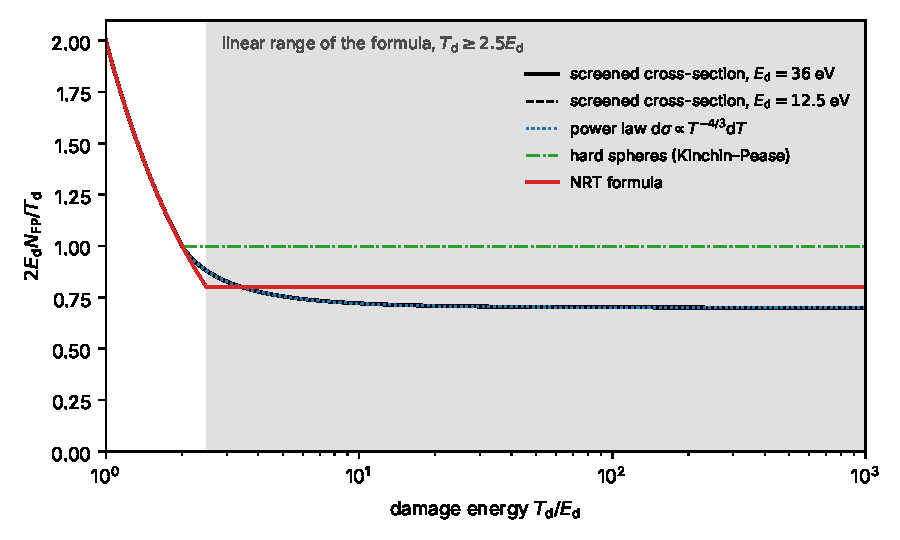
\includegraphics[width=\linewidth]{figures/ch19/limit19_4a.pdf}
\captionof{figure}{Displaced atoms per Kinchin--Pease unit, $2E_{\mathrm{d}}N_{\mathrm{FP}}/T_{\mathrm{d}}$, against $T_{\mathrm{d}}/E_{\mathrm{d}}$, from the counting equation \cref{eq:19.4-count} with the Kinchin--Pease rules, no binding energy and no electronic loss. Solid and dashed black: the Thomas--Fermi cross-section of \cref{sec:19.3} (impulse deflection, continued below $x_L = 2\times10^{-3}$ as $x_L^{1/3}$) for silicon with $E_{\mathrm{d}} = 36$ and \SI{12.5}{eV}; dotted: the power law $T^{-4/3}$; dash-dotted: hard spheres, which reproduce \cref{eq:19.4-KP} exactly. Red: the formula. Gray: $T_{\mathrm{d}} \ge 2.5E_{\mathrm{d}}$, the formula's linear range.}\label{fig:19-limit-nrt}
\par}
\smallskip
In its linear range the formula lies 11 to \SI{14}{\percent} above the screened count for $T_{\mathrm{d}} \ge 10E_{\mathrm{d}}$ and \SI{20}{\percent} below the hard-sphere count; below $2.5E_{\mathrm{d}}$ the count is set by the direction dependence of the threshold and by recombination, which no counting rule contains.
\end{limitbox}

The factor in front of the count is therefore a property of the cross-section and of the rules, not a constant of the crystal: 1 for hard spheres, 0.8 in the formula, 0.70 for the screened cross-section that \cref{sec:19.3} uses for Lindhard quenching. The rules leave out binding and recombination. A binding energy paid by every displaced atom lowers the count. Recombination inside a dense cascade lowers the number of defects that survive; in metals the surviving number from molecular dynamics is a third to a quarter of the formula's count~\cite{nordlund2018improving}, while silicon and germanium recombine much less~\cite[Sect.~II\,B]{sassi2022energy}.

The defect energy loss follows by multiplying the count by the surviving fraction and by the energy per pair. Writing $E_{\mathrm{FP}}$ for the mean stored energy of a surviving displacement,
\begin{equation}
  \frac{\langle E_{\mathrm{st}}\rangle}{E_R} = \frac{\xi_{\mathrm{d}}}{2}\,\frac{T_{\mathrm{d}}}{E_R}\,\frac{p_{\mathrm{surv}}E_{\mathrm{FP}}}{E_{\mathrm{d}}} \qquad (T_{\mathrm{d}} \gg E_{\mathrm{d}}) .
  \label{eq:19.4-loss}
\end{equation}
The stored fraction depends on the recoil energy only through the damage fraction $T_{\mathrm{d}}/E_R = 1 - y_L$, which falls from 0.70 at \SI{10}{keV} to 0.49 at \SI{100}{keV} for silicon in Lindhard's model, \cref{eq:16.6-lindhard}. At fixed $p_{\mathrm{surv}}E_{\mathrm{FP}}$ it decreases as $1/E_{\mathrm{d}}$: a higher threshold means fewer displacements, each storing the same energy. A measured stored fraction fixes only the combination $\xi_{\mathrm{d}}p_{\mathrm{surv}}E_{\mathrm{FP}}/E_{\mathrm{d}}$.

\begin{workedexample}{Energy stored by a 300 eV silicon recoil}\label{we:19-fp300}
A silicon recoil of \SI{300}{eV} needs $\mchi \ge \SI{0.770}{GeV}$ by \cref{eq:1.3-ERmax}, with $M_\kappa = \SI{26.16}{GeV}$ (natural isotope mixture, as in \cref{sec:19.1}) and $v_{\mathrm{max}} = \num{2.650e-3}$. Its measured ionization yield, interpolated linearly in $\ln Y_q$ against $\ln E_R$ between 0.108 at \SI{0.22}{keV} and 0.136 at \SI{0.46}{keV}~\cite[Table~II]{albakry2023first}, is $Y_q = 0.119$. The electronic share is at most $Y_qE_R = \SI{36}{eV}$, since the near-gap excitations of a slow ion each cost less than $\varepsilon_{\mathrm{eh}}$ per pair (\cref{sec:19.2}), so $T_{\mathrm{d}} \ge \SI{264}{eV}$; we take this value.

With the average Frenkel-pair threshold $E_{\mathrm{d}} = \SI{36}{eV}$, $T_{\mathrm{d}}/E_{\mathrm{d}} = 7.34$. The hard-sphere count \cref{eq:19.4-KP} gives 3.67 displacements, the formula of \cref{lim:19.4a} 2.94, and the screened count of \cref{eq:19.4-count} 2.69. If every displacement survives as a close pair of 6.8 to \SI{7.5}{eV}, the recoil stores 18.3 to \SI{20.1}{eV}, 6.1 to \SI{6.7}{\percent} of its energy; as separated pairs of 8.1 to \SI{9.7}{eV}, 22 to \SI{26}{eV}, or 7.3 to \SI{8.7}{\percent}. With the threshold for a defect of either kind, \SI{24}{eV}, the screened count is 3.95, and bond defects alone would store 10 to \SI{12}{eV}.

These fractions are comparable to the deficits measured at 10 to \SI{100}{keV}, and a calorimeter calibrated with electron recoils would read this recoil about \SI{20}{eV} low.
\end{workedexample}

\section{The energy balance law}\label{sec:19.5}

A silicon recoil of \SI{1}{keV} makes about 34 electron--hole pairs, at the measured ionization yield $Y_q = 0.127$ (\cref{sec:19.2}) and $\varepsilon_{\mathrm{eh}} = \SI{3.75}{eV}$, and their gap energy is \SI{40}{eV}. The rest of the deposit is phonons and, if the recoil displaced atoms, stored energy. A millisecond later the phonons have been absorbed at the surfaces of the crystal, most pairs have returned their gap energy as phonons and a few are caught on traps, while the defects still hold their energy. A phonon sensor reads the share that reached it within its readout window, and a calibration made with electron recoils converts that reading into an energy. The conversion is correct when electron and nuclear recoils of the same energy deliver the same share. To see when that holds, we write one law that tracks every share at every time. Applied to the silicon calibration of the CDMS~II detectors, the law shows that the measured ratio fixes a combination of stored energy, phonon collection and the pair energy of the reconstruction, which a second bias can separate.

\subsection{Reservoirs of the deposit}\label{sec:19.5-law}

At the partition time $t_{\mathrm{pr}}$ the deposit $\omega$ is split as in \cref{eq:19.1-heat}: $N_{\mathrm{eh}}\Eg$ in pairs, $E_{\mathrm{st}}$ in defects and $E_{\mathrm{heat}}$ in phonons. After $t_{\mathrm{pr}}$ the energy keeps moving. Pairs bind into excitons, recombine, are captured on impurities or drift to the electrodes, defects release their energy (\cref{sec:19.6}), and the phonons leave the crystal through its surfaces. Five reservoirs hold the energy at any time $t$. Write $E_{\mathrm{dep}} \equiv \omega$ for the deposit when it is divided among them.

The carriers hold $E_{\mathrm{pairs}}(t)$. Each energy is counted from the Fermi level $\mu_F$ of the electrodes, as in \cref{sec:18.5}: a free electron holds $E_c - \mu_F$, a free hole $\mu_F - E_v$, an exciton $\Eg - E_x^b$, an electron trapped on a level $E_j$ holds $E_j - \mu_F$ and a trapped hole $\mu_F - E_j$. To these we add the electrostatic energy of the charge left in the crystal, the Coulomb energy of separated carriers, their images in the electrodes and any space charge. The phonons hold $E_{\mathrm{phon}}(t)$, the vibrational energy above the thermal bath; its value at $t_{\mathrm{pr}}$ is the prompt phonon energy $E_{\mathrm{prompt}} \equiv E_{\mathrm{phon}}(t_{\mathrm{pr}})$. The defects hold the stored energy $E_{\mathrm{st}}(t)$, a difference of minima of $E^{\mathrm{ad}}$ as in \cref{eq:19.1-partition}. The escaped energy $E_{\mathrm{esc}}(t)$ is carried out of the crystal by quanta that no surface absorbs, in practice luminescence photons. Last, $E_{\mathrm{sens}}(t)$ is the energy absorbed at the surfaces: by the sensor films, of which a part becomes signal, and by holders and uninstrumented faces. A bias source at fixed voltage adds the work $W_{\mathrm{bias}}(t)$ it has done on the drifting charge.
\begin{keyresult}[Energy balance law]
At every time $t$ after the deposit, and for every event,
\begin{equation}
  E_{\mathrm{dep}} + W_{\mathrm{bias}}(t) =
  \underbrace{E_{\mathrm{pairs}}(t)}_{\text{carriers}} +
  \underbrace{E_{\mathrm{phon}}(t)}_{\text{phonons}} +
  \underbrace{E_{\mathrm{st}}(t)}_{\text{defects}} +
  \underbrace{E_{\mathrm{esc}}(t)}_{\text{escaped}} +
  \underbrace{E_{\mathrm{sens}}(t)}_{\text{absorbed}} ,
  \label{eq:19.5-balance}
\end{equation}
with carrier energies counted from the Fermi level of the electrodes, the stored energy configurational, and the change of zero-point energy of the occupied defect basins inside $E_{\mathrm{phon}}$.
\end{keyresult}
\noindent \Cref{app:D.45} proves \cref{eq:19.5-balance} from the conservation of the total energy of crystal, sensors, radiation and bias source. Apart from the work of the source, the total energy is conserved. Between collisions it equals the sum of the reservoir energies, since the interactions of excited carriers with each other are either long-range Coulomb energy, which $E_{\mathrm{pairs}}$ contains, or short-range energy that acts during a collision alone. Every process after $t_{\mathrm{pr}}$ is a short-range transition that conserves energy, or a drift whose energy the bias work and the electrostatic energy account for. The law holds for each realization of the random sequence of captures, hops and absorptions, and hence also in the mean. Its content is the completeness of the reservoir list. At $t_{\mathrm{pr}}$ and zero field, with no capture, it is the partition: $E_{\mathrm{pairs}} = N_{\mathrm{eh}}\Eg$, $E_{\mathrm{prompt}} = E_{\mathrm{heat}}$, $E_{\mathrm{esc}} = E_{\mathrm{sens}} = 0$, and \cref{eq:19.5-balance} is \cref{eq:19.1-heat}.

The Fermi level of the electrodes is the one reference for the carrier energies that keeps the law closed. A carrier that reaches an electrode gives up its energy relative to the Fermi level of that electrode, as phonons at the contact; the CDMS~II analysis names these the recombination phonons~\cite[Sect.~2]{agnese2018nuclear}. Counted from another level $\mu$, the carriers still in the crystal hold an energy whose derivative with respect to $\mu$ is the number of holes minus the number of electrons among them. That number is zero as long as every carrier still has its partner. Once one carrier of a pair has been collected and the other has not, energies counted from $\mu \ne \mu_F$ change with the arbitrary $\mu$, and the balance no longer closes. A hole left behind when its electron is collected thus stores $\mu_F - E_v$, plus its image energy, and not half the gap.

The stored energy enters once. The displacement threshold appears nowhere in \cref{eq:19.5-balance}. The stored energy decreases through releases alone, each of which moves its energy to $E_{\mathrm{phon}}$, or to $E_{\mathrm{esc}}$ if a photon carries it away. A calibration that subtracts an energy per displaced atom from the heat and also counts the later release as heat counts the same energy twice.

The zero-point energy of the occupied basins sits inside $E_{\mathrm{phon}}$. A defect softens or stiffens the modes of its neighbors and so changes the zero-point energy of the crystal by an amount $\Delta E_{\mathrm{zp}}(t)$, which \cref{sec:19.1-partition} placed in the lattice share. It is the energy of the vibrational ground state, and no sensor can absorb it. Its size follows from the zero-point energy per silicon atom, $3\langle\omega\rangle/2 = \SI{61}{meV}$, half of it the potential energy of \cref{sec:19.1-md}. A point defect that shifts the frequencies of its four neighbors by some tens of percent changes $\Delta E_{\mathrm{zp}}$ by about \SI{0.07}{eV}, an estimate, against the several eV a Frenkel pair stores. The sign is not fixed: softened modes make $\Delta E_{\mathrm{zp}}$ negative, stiffened ones positive. A defect that hops from basin $i$ to basin $j$ releases into the phonons the configurational difference plus the change of zero-point energy between the two basins. Summed along any release path, the zero-point terms telescope like the configurational ones, so the sum rule of \cref{sec:19.6} holds for both separately. A sensor can draw on $E_{\mathrm{phon}} - \Delta E_{\mathrm{zp}}$ alone.

The Luke effect enters the balance through the bias work. A carrier drifting at constant velocity in the field of a biased detector gains from the field the energy $e\mathcal{E}$ per unit path and gives it to phonons as fast as it gains it: the Neganov--Trofimov--Luke effect of \cref{eq:1.5-luke}, whose emission spectrum \cref{sec:20.1} treats. Between two planar electrodes at fixed potentials, a carrier that crosses a fraction $s$ of the gap induces the charge $es$ on the electrodes, and the source does the work $eV_{\mathrm{bias}}s$ on it (Ramo's theorem, \cref{app:D.45}). The total work is
\begin{equation}
  W_{\mathrm{bias}} = eV_{\mathrm{bias}}N_{\mathrm{ind}} ,
  \label{eq:19.5-Wbias}
\end{equation}
where $N_{\mathrm{ind}}$ is the induced charge in units of $e$, equal to the number of pairs if all are collected and smaller if carriers are trapped on the way. Of this work, $W_{\mathrm{bias}}$ minus the change of the electrostatic energy goes to phonons; for pairs born neutral and fully collected the electrostatic term vanishes at the end. For an electron recoil, whose pair number is $\omega/\varepsilon_{\mathrm{eh}}$, the ratio of the Luke phonon energy to the deposit is the Luke gain
\begin{equation*}
  g_{\mathrm{Luke}} = \frac{eV_{\mathrm{bias}}}{\varepsilon_{\mathrm{eh}}} ,
\end{equation*}
1.07 at \SI{4}{V} and 26.7 at \SI{100}{V} in silicon. Carriers already drift during the cascade, before $t_{\mathrm{pr}}$, over the short distance they travel in that time; that work is part of the same $W_{\mathrm{bias}}$ and of the same Luke phonons.

\Cref{fig:19-shares} follows the five reservoirs of a \SI{1}{keV} silicon recoil at zero field. The pair kinetics are those of \cref{fig:18-end}: the gap energy is released within microseconds, except for the \SI{5}{\percent} of pairs that the illustrative rates trap and the \SI{0.9}{\percent} that leave as light. The phonons are absorbed with a single time constant of \SI{58}{\micro s}, the fall time of the pulse of a \SI{10.6}{g} silicon phonon detector~\cite[p.~2]{alkhatib2021light}. After a millisecond the surfaces have absorbed \SI{943}{eV}, the traps keep \SI{2.0}{eV} and the defects their full \SI{55}{eV}. For a stated detector the evolution of the reservoirs is a transport calculation: the charge kinetics, Luke emission and collection at the surfaces of \cref{app:E.25}, started from the partition tables of \cref{app:E.23}.

\begin{figure}[tbp]
  \centering
  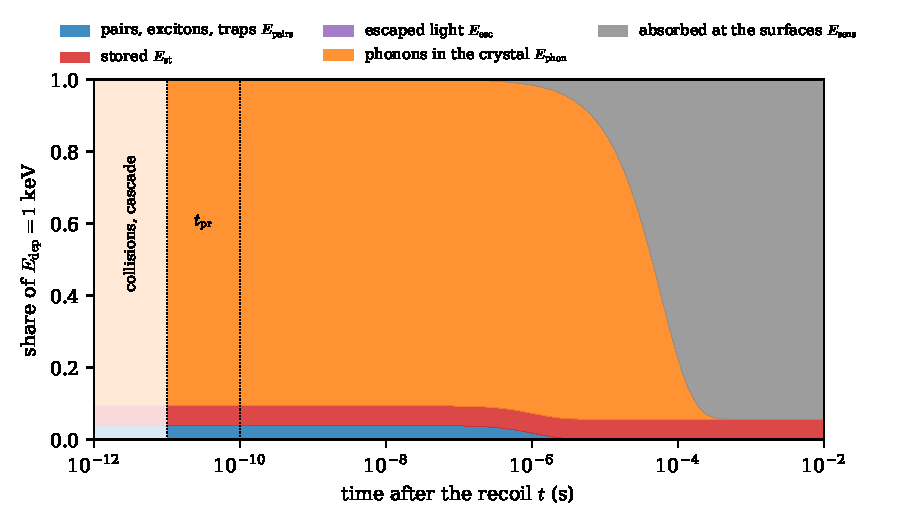
\includegraphics[width=\linewidth]{figures/ch19/fig19_4.pdf}
  \caption{Shares of the balance law \cref{eq:19.5-balance} for a \SI{1}{keV} silicon recoil at zero field, against the time after the recoil, as fractions of $E_{\mathrm{dep}}$. At the partition time $t_{\mathrm{pr}}$ (dotted lines, 10 to \SI{100}{ps}): $N_{\mathrm{eh}} = 33.9$ pairs from the measured yield $Y_q = 0.127$ at \SI{0.89}{keV}~\cite[Table~II]{albakry2023first} with $\varepsilon_{\mathrm{eh}} = \SI{3.75}{eV}$, holding $N_{\mathrm{eh}}\Eg = \SI{39.6}{eV}$ with $\Eg = \SI{1.17}{eV}$; stored energy set to \SI{55}{eV}, the silicon bound of \cref{tab:19-bounds}, for display, and kept frozen; phonons \SI{905}{eV}. Pair kinetics: the illustrative rates of \cref{fig:18-end} (one free pair per pair, \SI{5}{\percent} trapped, luminescent fraction 0.1 of free-exciton decay, bound-exciton Auger decay \SI{250}{ns}); trapped carriers stay in $E_{\mathrm{pairs}}$. Phonons absorbed at the surfaces with one exponential time constant, \SI{58}{\micro s}, the pulse fall time of a silicon phonon detector~\cite[p.~2]{alkhatib2021light}, a modeling choice. Shares at \SI{10}{ms}: absorbed 0.943, stored 0.055, trapped 0.002, escaped $3\times10^{-4}$. The collisions and the cascade before $t_{\mathrm{pr}}$ are not resolved.}
  \label{fig:19-shares}
\end{figure}

\subsection{Heat quenching}\label{sec:19.5-heat}

Without bias the phonon sensors measure the heat. Their readout integrates the energy absorbed during a window $t_{\mathrm{win}}$, from microseconds to a second depending on the sensor, and the phonons still in the crystal at the end of the window are absorbed with the same pulse shape whatever made them. Energy that has not become available phonons by $t_{\mathrm{win}}$ is missing from the signal for good. It is the sum of the energy still held by carriers, the energy still stored, the escaped energy and the zero-point change,
\begin{equation*}
  E_{\mathrm{miss}}(t_{\mathrm{win}}) = E_{\mathrm{pairs}}(t_{\mathrm{win}}) + E_{\mathrm{st}}(t_{\mathrm{win}}) + E_{\mathrm{esc}}(t_{\mathrm{win}}) + \Delta E_{\mathrm{zp}}(t_{\mathrm{win}}) .
\end{equation*}
The sensors turn a fraction $\epsilon_{\mathrm{abs}}$ of the available phonon energy into signal, $\epsilon_{\mathrm{abs}}(E_{\mathrm{dep}} - E_{\mathrm{miss}})$; the rest goes into $E_{\mathrm{sens}}$ as loss on uninstrumented faces and in the films. This fraction is often well below one, but it is the same for every event of a given kind of recoil at a given place. Let $\epsilon^{\mathrm{NR}}_{\mathrm{prim}}$ and $\epsilon^{\mathrm{ER}}_{\mathrm{prim}}$ be its values for the primary phonons of nuclear and electron recoils, the sole phonons at zero field, and define the collection offset $\delta_{\mathrm{coll}} \equiv 1 - \epsilon^{\mathrm{NR}}_{\mathrm{prim}}/\epsilon^{\mathrm{ER}}_{\mathrm{prim}}$. The heat quenching is the ratio of the heat signals of a nuclear and an electron recoil of the same energy,
\begin{equation}
  Y_{\mathrm{ph}}(0) = (1 - \delta_{\mathrm{coll}})\,\frac{1 - d_{\mathrm{NR}}}{1 - d_{\mathrm{ER}}} , \qquad
  d_{\mathrm{NR},\mathrm{ER}} \equiv \frac{E^{\mathrm{NR},\mathrm{ER}}_{\mathrm{miss}}(t_{\mathrm{win}})}{\omega} ,
  \label{eq:19.5-heatq}
\end{equation}
the zero-field value of the phonon-yield ratio $Y_{\mathrm{ph}}$ defined in \cref{sec:19.5-yield}. The absolute efficiency has dropped out, and with it the large losses at the surfaces; what remains is the difference between the two kinds of recoil.

Unit heat quenching, $Y_{\mathrm{ph}}(0) = 1$, is the truncation that phonon-only searches use to read a nuclear-recoil energy from a scale calibrated with electron recoils~\cite[p.~4]{alkhatib2021light}. \Cref{eq:19.5-heatq} states what it requires: equal collection of the two phonon populations, $\delta_{\mathrm{coll}} = 0$, and equal missing energy, $d_{\mathrm{NR}} = d_{\mathrm{ER}}$. The second condition does not hold by accident. An electron recoil puts the fraction $\Eg/\varepsilon_{\mathrm{eh}} = 0.312$ of its energy into pair gap energy, a silicon recoil of \SI{100}{eV} a fraction $Y_q$ times as large, so the two missing energies are equal when both are zero. The truncation therefore holds when, within the read window, every pair has recombined or been collected with its gap energy returned as phonons, no defect holds energy, and nothing has escaped.

The gap-energy term is the one that depends on the window. Let $f_{\mathrm{ret}}(t)$ be the fraction of the gap energy of the pairs returned as phonons by the time $t$, and $1 - f_{\mathrm{ret}}(t)$ the rest: held by free pairs and excitons, $r_{\mathrm{gap}}(t)$ of \cref{eq:18.5-rgap}, plus what has gone to traps and to light. The nuclear recoil holds $Y_q$ times the pair energy of the electron recoil. At zero field \cref{eq:19.5-heatq} becomes the gap-energy release law
\begin{equation}
  Y_{\mathrm{ph}}(0) = (1 - \delta_{\mathrm{coll}})\,\frac{1 - Y_q\,(\Eg/\varepsilon_{\mathrm{eh}})(1 - f^{\mathrm{NR}}_{\mathrm{ret}}) - (E_{\mathrm{st}} + \Delta E_{\mathrm{zp}})/\omega}{1 - (\Eg/\varepsilon_{\mathrm{eh}})(1 - f^{\mathrm{ER}}_{\mathrm{ret}})} ,
  \label{eq:19.5-release}
\end{equation}
with $f_{\mathrm{ret}}$, $E_{\mathrm{st}}$ and $\Delta E_{\mathrm{zp}}$ taken at $t_{\mathrm{win}}$ and the escape of light counted in $1 - f_{\mathrm{ret}}$. Nothing in it is small. If no gap energy has come back, $f_{\mathrm{ret}} = 0$, a silicon recoil of \SI{100}{eV} with $Y_q = 0.102$ has $Y_{\mathrm{ph}}(0) = 0.968/0.688 = 1.407$. Its heat signal is \SI{41}{\percent} larger than that of an electron recoil of the same energy, because the electron recoil holds more of its energy in pairs. The first-order form, $1 + (1 - Y_q)(\Eg/\varepsilon_{\mathrm{eh}})(1 - f_{\mathrm{ret}})$, is 1.280 and not usable at this size. With the illustrative rates of \cref{fig:18-end}, a window of \SI{1}{\micro s} has $f_{\mathrm{ret}} = 0.525$ and $Y_{\mathrm{ph}}(0) = 1.156$; after \SI{10}{\micro s} all free pairs and excitons have decayed, $f_{\mathrm{ret}} = 0.941$, and the \SI{5.9}{\percent} that went to traps and to light leave $Y_{\mathrm{ph}}(0) = 1.017$ at any longer window. The trapped fraction never comes back at millikelvin, where emission from traps is frozen (\cref{sec:18.5-kinetics}).

When the kinetics are linear, each pair decays on its own and $f^{\mathrm{NR}}_{\mathrm{ret}} = f^{\mathrm{ER}}_{\mathrm{ret}}$ at every time, a sum of exponentials whose rates are those of \cref{eq:18.5-rates}. The tracks of nuclear recoils are denser than the clouds of electron recoils of the same energy, however, and in a dense track the pairs meet. Binding of carriers from different pairs moves gap energy from free pairs into excitons and changes nothing in $1 - f_{\mathrm{ret}}$. Two-body processes that return gap energy to the lattice do: two excitons that meet annihilate, one of them giving up its energy, and three free carriers recombine by the Auger process. Write $\nd(t)$ for the density of pairs in the track, $\nd_0$ for its initial value, and take $1 - f_{\mathrm{ret}} \simeq \nd/\nd_0$ while no other channel acts. Annihilation gives $\dd\nd/\dd t = -\nd^2/(\nd_0t_0)$, and Auger recombination $\dd\nd/\dd t = -\nd^3/(2\nd_0^2t_0)$, with $t_0$ the time scale each sets at the initial density. Integrating,
\begin{equation}
  1 - f_{\mathrm{ret}}(t) = \frac{1}{1 + t/t_{\mathrm{rel}}}\ \ \text{(annihilation)} , \qquad
  1 - f_{\mathrm{ret}}(t) = \Bigl(1 + \frac{t}{t_{\mathrm{rel}}}\Bigr)^{-1/2}\ \ \text{(Auger)} .
  \label{eq:19.5-bimol}
\end{equation}
At $t_{\mathrm{win}} \gg t_{\mathrm{rel}}$ the nuclear recoil then misses $Y_q(\Eg/\varepsilon_{\mathrm{eh}})\,t_{\mathrm{rel}}/t_{\mathrm{win}}$ or $Y_q(\Eg/\varepsilon_{\mathrm{eh}})(t_{\mathrm{rel}}/t_{\mathrm{win}})^{1/2}$ of its energy, a power of the window and not an exponential, with $t_{\mathrm{rel}}$ set by the density of its own track. The heat quenching of nuclear recoils depends on the window whenever a two-body channel acts within it. Diffusion dilutes a track as it decays, and a compact cloud then stops losing energy by two-body processes and returns to the linear law, so \cref{eq:19.5-bimol} holds while the track stays narrow. The rates that decide which regime a detector is in are not known at millikelvin (\cref{sec:18.5-open}); \cref{app:E.24,app:E.25} specify their calculation.

\begin{limitbox}[Unit heat quenching][lim:19.5a]
The heat signals of nuclear and electron recoils of the same energy are taken to be equal~\cite[p.~4]{alkhatib2021light}: $Y_{\mathrm{ph}}(0) = 1$.
\par\smallskip
{\centering
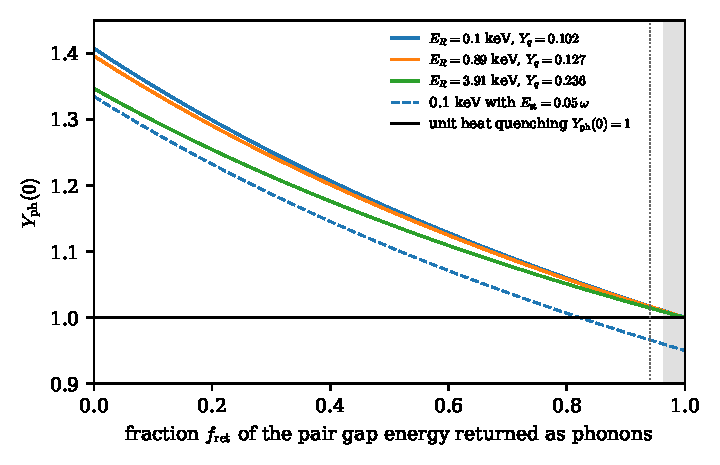
\includegraphics[width=\linewidth]{figures/ch19/limit19_5a.pdf}
\captionof{figure}{Heat quenching of silicon recoils from the release law \cref{eq:19.5-release} with $\delta_{\mathrm{coll}} = 0$, $\Delta E_{\mathrm{zp}} = 0$ and the same returned fraction $f_{\mathrm{ret}}$ for both recoils, against $f_{\mathrm{ret}}$. Solid: no stored energy, at the measured yields $Y_q$~\cite[Table~II]{albakry2023first} of 0.10, 0.89 and \SI{3.91}{keV}; $\Eg = \SI{1.17}{eV}$, $\varepsilon_{\mathrm{eh}} = \SI{3.75}{eV}$. Dashed: \SI{0.1}{keV} with a stored energy of $0.05\,\omega$. Horizontal line: the truncation. Gray: $f_{\mathrm{ret}} \ge 0.965$, where the \SI{0.1}{keV} curve lies within \SI{1}{\percent} of one. Dotted: $f_{\mathrm{ret}} = 0.941$, the asymptotic phonon share of the illustrative kinetics of \cref{fig:18-end}; there \SI{5}{\percent} of the pairs are trapped.}\label{fig:19-limit-heat}
\par}
\smallskip
When part of the gap energy is still held by pairs, excitons or traps at the end of the window, the electron recoil, with four to ten times more energy in pairs, loses more of its heat than the nuclear recoil, and the ratio rises above one, by up to \SI{41}{\percent} at \SI{100}{eV}; stored energy pulls it below.
\end{limitbox}

The truncation demands nearly complete release. Within \SI{1}{\percent} at \SI{100}{eV} requires $1 - f_{\mathrm{ret}} \le 0.035$, and the bound is nearly the same over the measured range, 0.036 at \SI{0.89}{keV} and 0.041 at \SI{3.91}{keV}, since the factor $(1 - Y_q)$ changes little while $Y_q$ stays small. A trapped fraction of a few percent, which no window removes, is already a percent-level violation, of opposite sign to the stored energy. The two effects can cancel in a single measurement, which is one reason a heat measurement alone determines neither.

\subsection{The phonon-yield ratio}\label{sec:19.5-yield}

With a bias the phonon signal has three parts: the primary phonons of the recoil, the Luke phonons of the drift and the recombination phonons that carriers emit at the contacts~\cite[Sect.~2]{agnese2018nuclear}. The recombination phonons carry gap energy returned within the window, and the balance law counts them with the primaries, in $E_{\mathrm{dep}} - E_{\mathrm{miss}}$; when drift collects the pairs within the window, $E_{\mathrm{miss}}$ holds the trapped carriers and their electrostatic energy, and the stored, escaped and zero-point energy. The sensors collect primary and Luke phonons with different efficiencies, because the two populations are born with different spectra and in different places. Let $\epsilon^{\mathrm{ER}}_{\mathrm{prim}}$ and $\epsilon^{\mathrm{NR}}_{\mathrm{prim}} = (1 - \delta_{\mathrm{coll}})\epsilon^{\mathrm{ER}}_{\mathrm{prim}}$ be the efficiencies for the primary phonons of the two recoils and $\epsilon_{\mathrm{Luke}}$ that for Luke phonons, and define the collection ratio
\begin{equation*}
  \mathfrak{r}_{\mathrm{coll}} \equiv \frac{\epsilon_{\mathrm{Luke}}}{\epsilon^{\mathrm{ER}}_{\mathrm{prim}}} ,
\end{equation*}
the efficiency for Luke phonons over that for the primary phonons of an electron recoil. Let the electron recoil be fully collected, so that its bias work is $g_{\mathrm{Luke}}\omega$ by \cref{eq:19.5-Wbias}, and define the ionized fraction $f_{\mathrm{ion}}$ of a nuclear recoil as its bias work over that of an electron recoil of the same energy, $f_{\mathrm{ion}} = N^{\mathrm{NR}}_{\mathrm{ind}}/N^{\mathrm{ER}}_{\mathrm{ind}}$. It equals the ionization yield $Y_q$ of \cref{eq:19.2-Yq} when both recoils are collected alike and is smaller if the carriers of the dense track are trapped more often. Per unit deposit the two signals are then
\begin{equation}
  \frac{S_{\mathrm{ER}}}{\epsilon^{\mathrm{ER}}_{\mathrm{prim}}\,\omega} = 1 - d_{\mathrm{ER}} + \mathfrak{r}_{\mathrm{coll}}\,g_{\mathrm{Luke}} , \qquad
  \frac{S_{\mathrm{NR}}}{\epsilon^{\mathrm{ER}}_{\mathrm{prim}}\,\omega} = (1 - \delta_{\mathrm{coll}})(1 - d_{\mathrm{NR}}) + \mathfrak{r}_{\mathrm{coll}}\,g_{\mathrm{Luke}}f_{\mathrm{ion}} .
  \label{eq:19.5-signal}
\end{equation}

The CDMS~II calibration turns these signals into energies in two steps~\cite[Eq.~(1), Sect.~2.1]{agnese2018nuclear}. The charge channel is calibrated with photon lines, so that an electron recoil of energy $\omega$ reads the electron-equivalent energy $E_Q = \omega$ and a nuclear recoil $E_Q = f_{\mathrm{ion}}\omega$. The phonon scale is set with bulk electron recoils, taken to have unit ionization yield, so that an electron recoil reads $E_\phi = \omega(1 + eV_{\mathrm{bias}}/\varepsilon_{\mathrm{cal}})$, and a nuclear recoil is assigned the energy $E_\phi - E_QeV_{\mathrm{bias}}/\varepsilon_{\mathrm{cal}}$. Note that $\varepsilon_{\mathrm{cal}}$ is the pair energy the reconstruction adopts, \SI{3.82}{eV} for silicon~\cite[Sect.~2]{agnese2018nuclear}, not the true $\varepsilon_{\mathrm{eh}}$. It enters both the scale and the subtraction, through the gain $g_{\mathrm{cal}} \equiv eV_{\mathrm{bias}}/\varepsilon_{\mathrm{cal}}$, while the Luke phonons follow the true pair number and $g_{\mathrm{Luke}}$. The phonon-yield ratio $Y_{\mathrm{ph}}$ is the reconstructed energy of the nuclear recoil over its true energy, which the CDMS~II analysis calls the phonon collection efficiency for nuclear recoils relative to electron recoils, and its deficit is the defect fraction $f_{\mathrm{DF}} \equiv 1 - Y_{\mathrm{ph}}$. From \cref{eq:19.5-signal},
\begin{equation}
  Y_{\mathrm{ph}} = (1 + g_{\mathrm{cal}})\,\frac{(1 - \delta_{\mathrm{coll}})(1 - d_{\mathrm{NR}}) + \mathfrak{r}_{\mathrm{coll}}g_{\mathrm{Luke}}f_{\mathrm{ion}}}{1 - d_{\mathrm{ER}} + \mathfrak{r}_{\mathrm{coll}}g_{\mathrm{Luke}}} - f_{\mathrm{ion}}g_{\mathrm{cal}} .
  \label{eq:19.5-identity}
\end{equation}
The absolute efficiency $\epsilon^{\mathrm{ER}}_{\mathrm{prim}}$ has cancelled. With no missing energy and $\mathfrak{r}_{\mathrm{coll}} = 1$ the ratio is $1 + (g_{\mathrm{cal}} - g_{\mathrm{Luke}})(1 - f_{\mathrm{ion}})/(1 + g_{\mathrm{Luke}})$, not one. For silicon at \SI{4}{V}, with $g_{\mathrm{Luke}} = 1.067$, $g_{\mathrm{cal}} = 1.047$ and $f_{\mathrm{ion}} = 0.324$, the pair energy alone produces a deficit of 0.0064, against the half-width 0.008 of the measured band. At zero bias \cref{eq:19.5-identity} is the heat quenching \cref{eq:19.5-heatq}, and multiplying out its denominator relates the two.
\begin{keyresult}[Calibration identity]
The phonon-yield ratio at bias $V_{\mathrm{bias}}$ and the heat quenching $Y_{\mathrm{ph}}(0)$ of the same recoils, with the same missing energies, are related by
\begin{equation}
  Y_{\mathrm{ph}} = \frac{(1 + g_{\mathrm{cal}})\,Y_{\mathrm{ph}}(0) + f_{\mathrm{ion}}(\mathfrak{r}'g_{\mathrm{Luke}} - g_{\mathrm{cal}})}{1 + \mathfrak{r}'g_{\mathrm{Luke}}} , \qquad
  \mathfrak{r}' = \frac{\mathfrak{r}_{\mathrm{coll}}}{1 - d_{\mathrm{ER}}} .
  \label{eq:19.5-calib}
\end{equation}
When $\mathfrak{r}'g_{\mathrm{Luke}} = g_{\mathrm{cal}}$, the calibrated ratio equals the heat quenching at every bias; for a reconstruction with the true pair energy this is $\mathfrak{r}' = 1$, Luke phonons collected like the available primary phonons of an electron recoil.
\end{keyresult}
\noindent The ratio $\mathfrak{r}'$ differs from $\mathfrak{r}_{\mathrm{coll}}$ by the missing energy of the calibrating electron recoils. Flashing, the exposure of the detectors to infrared light that neutralizes ionized traps before data taking~\cite[Sect.~2]{agnese2018nuclear}, keeps that energy small. Away from $\mathfrak{r}'g_{\mathrm{Luke}} = g_{\mathrm{cal}}$ the two ratios differ even when no energy is missing, since the Luke phonons, a larger share of the electron-recoil signal than of the nuclear one, then carry a different weight in the two.

The expansion of \cref{eq:19.5-identity} to first order in $\delta_{\mathrm{coll}}$ and the missing energies, derived in \cref{app:D.45}, displays the separate contributions:
\begin{equation}
\begin{split}
  1 - Y_{\mathrm{ph}} &= \frac{(\mathfrak{r}_{\mathrm{coll}}g_{\mathrm{Luke}} - g_{\mathrm{cal}})(1 - f_{\mathrm{ion}})}{1 + \mathfrak{r}_{\mathrm{coll}}g_{\mathrm{Luke}}} + \frac{1 + g_{\mathrm{cal}}}{1 + \mathfrak{r}_{\mathrm{coll}}g_{\mathrm{Luke}}}\bigl[\delta_{\mathrm{coll}} + d_{\mathrm{NR}} - C_{\mathrm{cal}}\,d_{\mathrm{ER}}\bigr] , \\
  C_{\mathrm{cal}} &= \frac{1 + \mathfrak{r}_{\mathrm{coll}}g_{\mathrm{Luke}}f_{\mathrm{ion}}}{1 + \mathfrak{r}_{\mathrm{coll}}g_{\mathrm{Luke}}} .
\end{split}
  \label{eq:19.5-first}
\end{equation}
The collection term is exact, and it is the whole answer when no energy is missing; it contains the pair-energy offset $g_{\mathrm{Luke}} - g_{\mathrm{cal}}$ together with $\mathfrak{r}_{\mathrm{coll}} - 1$. The calibration coefficient $C_{\mathrm{cal}}$ measures how much a deficit of the calibrating electron recoils matters. Such a deficit lowers the phonon scale and so raises every reconstructed nuclear-recoil energy. However, it acts through the primary part of the signal alone, and the nuclear recoil has less Luke signal to offset; as a result $C_{\mathrm{cal}} < 1$. For silicon at $\mathfrak{r}_{\mathrm{coll}} = 1$ and $f_{\mathrm{ion}} = 0.324$ it is 0.651 at \SI{4}{V} and 0.382 at \SI{40}{V}, and 0.62 to 0.74 at \SI{4}{V} for the ionized fractions of 10 to \SI{100}{keV}. Since \cref{eq:19.5-identity} is linear in $\delta_{\mathrm{coll}}$ and in $d_{\mathrm{NR}}$ separately, the first-order form errs through their product and through $d_{\mathrm{ER}}$: by at most $3.0\times10^{-3}$ when each of the three lies between 0 and 0.05.

Write the missing energy of the nuclear recoil as $d_{\mathrm{NR}} = e_{\mathrm{st}} + x_{\mathrm{NR}}$, with $e_{\mathrm{st}} \equiv E_{\mathrm{st}}/\omega$ the stored fraction, and $x_{\mathrm{ER}} = d_{\mathrm{ER}}$ for the electron recoil, so that $x$ collects trapped, escaped and zero-point energy. Electron recoils store almost no energy. The largest energy an electron of kinetic energy $E$ gives a silicon nucleus is $2E(E + 2m_e)/M_\kappa$, which reaches the lowest threshold, \SI{12.5}{eV}, at $E = \SI{0.14}{MeV}$; whatever the calibrating electrons do store counts in $x_{\mathrm{ER}}$. \Cref{app:D.45} shows that \cref{eq:19.5-identity} implies, without approximation,
\begin{multline}
  (1 - Y_{\mathrm{ph}} - e_{\mathrm{st}})(1 - x_{\mathrm{ER}} + \mathfrak{r}_{\mathrm{coll}}g_{\mathrm{Luke}}) = (\mathfrak{r}_{\mathrm{coll}}g_{\mathrm{Luke}} - g_{\mathrm{cal}})(1 - e_{\mathrm{st}} - f_{\mathrm{ion}}) \\
  + (1 + g_{\mathrm{cal}})\bigl[\delta_{\mathrm{coll}}(1 - e_{\mathrm{st}}) + (1 - \delta_{\mathrm{coll}})x_{\mathrm{NR}}\bigr] - (1 - e_{\mathrm{st}} + f_{\mathrm{ion}}g_{\mathrm{cal}})\,x_{\mathrm{ER}} .
  \label{eq:19.5-bound}
\end{multline}
The factor $1 - x_{\mathrm{ER}} + \mathfrak{r}_{\mathrm{coll}}g_{\mathrm{Luke}}$ is positive. The right side is non-negative, and the stored fraction is therefore at most the defect fraction, $E_{\mathrm{st}}/\omega \le 1 - Y_{\mathrm{ph}}$, under five conditions on collection, missing energy and the reconstruction:
\begin{description}
\item[(a)] $\delta_{\mathrm{coll}} \ge 0$: the primary phonons of nuclear recoils are collected no better than those of electron recoils.
\item[(b)] $\mathfrak{r}_{\mathrm{coll}} \ge 1$: Luke phonons are collected no worse than the primaries of electron recoils.
\item[(c)] $(1 + g_{\mathrm{cal}})(1 - \delta_{\mathrm{coll}})x_{\mathrm{NR}} \ge (1 - e_{\mathrm{st}} + f_{\mathrm{ion}}g_{\mathrm{cal}})x_{\mathrm{ER}}$: at small deficits, the other missing energy of the nuclear recoil is at least $(1 + f_{\mathrm{ion}}g_{\mathrm{cal}})/(1 + g_{\mathrm{cal}})$ times that of the electron recoil. It holds, for instance, when the electron recoils lose nothing to traps after flashing and the zero-point change of the defects is not negative.
\item[(d)] $e_{\mathrm{st}} \le 1 - f_{\mathrm{ion}}$, met with a wide margin at stored fractions of a few percent.
\item[(e)] $\varepsilon_{\mathrm{eh}} \le \varepsilon_{\mathrm{cal}}$: the true pair energy is no larger than the one the reconstruction adopts, so that with (b) $\mathfrak{r}_{\mathrm{coll}}g_{\mathrm{Luke}} \ge g_{\mathrm{cal}}$. For germanium it refers to the pair energy of the germanium analysis, whose offset is not evaluated here.
\end{description}
The measured silicon pair energy, \SI{3.75}{eV} (\cref{sec:18.4}), meets (e) against the \SI{3.82}{eV} of the CDMS~II reconstruction; were $\varepsilon_{\mathrm{eh}}$ above $\varepsilon_{\mathrm{cal}}$, the first term would turn negative and the bound would loosen. At \SI{95}{\percent} confidence the silicon datum has $Y_{\mathrm{ph}} \ge 0.945$, so $E_{\mathrm{st}}/\omega \le 0.055$ under (a)--(e). With the book's $\varepsilon_{\mathrm{eh}}$ the pair-energy term is known, and under (a)--(d) the bound is tighter, 0.049, attained at $\mathfrak{r}_{\mathrm{coll}} = 1$ with no other deficit, since the first term of \cref{eq:19.5-bound} grows with $\mathfrak{r}_{\mathrm{coll}}$. A negative zero-point change violates (c) and widens the bound by $|\Delta E_{\mathrm{zp}}|/\omega$. With \SI{0.1}{eV} per displacement and the displacement count of \cref{lim:19.4a}, that is $8\times10^{-4}$ at \SI{10}{keV}, and the bound for either sign of $\Delta E_{\mathrm{zp}}$ is 0.056. \Cref{sec:19.4} collects the silicon and germanium bounds in \cref{tab:19-bounds}.

Condition (b) is the weak one. Luke phonons are emitted with energies of a few meV at most, softer than the primary phonons. In the films that collect phonons, the part of their spectrum below the pair-breaking energy $2\Delta_{\mathrm{BCS}}$ of aluminum, \SI{0.36}{meV} (\cref{sec:1.5}), is lost energy, as is the part absorbed at bare surfaces. The sign of $\mathfrak{r}_{\mathrm{coll}} - 1$ is therefore not fixed by the balance law. The mean-field transport estimate of \cref{sec:20.5-sign} puts the collection ratio between 0.81 and 1.02, and between 0.82 and 1.01 at the mean Luke energy of silicon electrons at \SI{1}{V/cm}, for one or two films of any thickness down to \SI{60}{nm} with energy conserved; values up to 1.5 arise only for a selective sink that the estimate does not identify in a detector. For a stated detector \cref{app:E.25} specifies the calculation. On the branch $\mathfrak{r}_{\mathrm{coll}} < 1$, with $\delta_{\mathrm{coll}} = x_{\mathrm{NR}} = x_{\mathrm{ER}} = 0$, \cref{eq:19.5-identity} solved for the stored energy is
\begin{equation}
  \frac{E_{\mathrm{st}}}{\omega} = 1 - Y_{\mathrm{ph}} + \frac{(g_{\mathrm{cal}} - \mathfrak{r}_{\mathrm{coll}}g_{\mathrm{Luke}})(Y_{\mathrm{ph}} - f_{\mathrm{ion}})}{1 + g_{\mathrm{cal}}} ,
  \label{eq:19.5-widen}
\end{equation}
so the inferred stored fraction grows linearly as $\mathfrak{r}_{\mathrm{coll}}$ falls. For the central silicon datum it is 0.042 at $\mathfrak{r}_{\mathrm{coll}} = 1$, 0.058 at 0.95 and 0.075 at 0.9, and the \SI{95}{\percent} bound reaches 0.081 at 0.9. The bound is void if nothing bounds $\mathfrak{r}_{\mathrm{coll}}$ from below.

\begin{limitbox}[Stored energy from the phonon-yield ratio][lim:19.5b]
The defect fraction read as stored energy~\cite[Eq.~(4)]{agnese2018energy}, \cite[Eq.~(1)]{agnese2018nuclear}: $E_{\mathrm{st}}/\omega = f_{\mathrm{DF}} = 1 - Y_{\mathrm{ph}}$, the case $\mathfrak{r}_{\mathrm{coll}} = 1$, $\delta_{\mathrm{coll}} = x_{\mathrm{NR}} = x_{\mathrm{ER}} = 0$, $\varepsilon_{\mathrm{cal}} = \varepsilon_{\mathrm{eh}}$ of \cref{eq:19.5-identity}, with $Y_{\mathrm{ph}} = 0.952^{+0.009}_{-0.007}$ (\SI{95}{\percent} C.L.) measured in silicon at \SI{4}{V}~\cite[Sect.~4]{agnese2018nuclear}.
\par\smallskip
{\centering
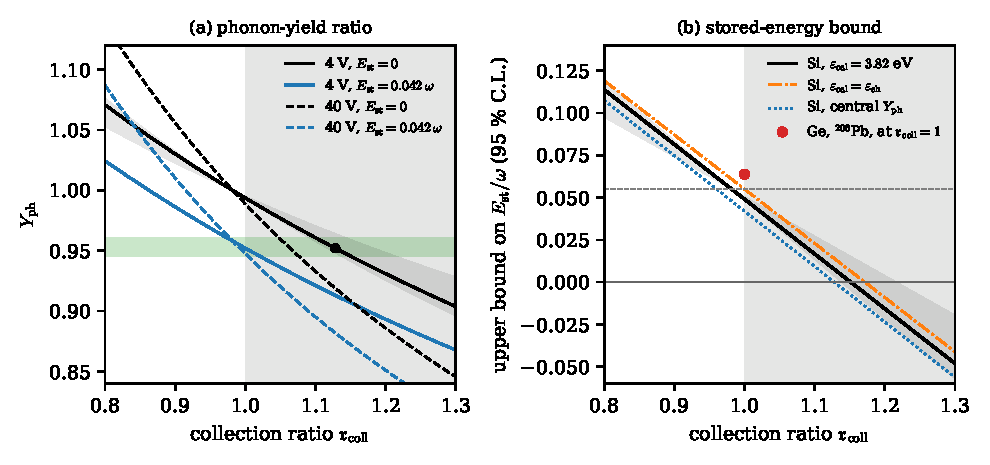
\includegraphics[width=\linewidth]{figures/ch19/limit19_5b.pdf}
\captionof{figure}{Silicon recoils against the collection ratio, from the exact identity \cref{eq:19.5-identity} with $\delta_{\mathrm{coll}} = d_{\mathrm{ER}} = 0$, $g_{\mathrm{Luke}} = 1.067$ ($\varepsilon_{\mathrm{eh}} = \SI{3.75}{eV}$) and $g_{\mathrm{cal}} = 1.047$ ($\varepsilon_{\mathrm{cal}} = \SI{3.82}{eV}$) at \SI{4}{V}, ten times both at \SI{40}{V}, and $f_{\mathrm{ion}} = 0.324$, the yield parameterization of the measurement at the \SI{20}{keV} resonance that dominates the calibration~\cite[Eq.~(4)]{agnese2018nuclear}. (a) Phonon-yield ratio. Black: no stored energy; blue: stored fraction 0.042; solid at \SI{4}{V}, dashed at \SI{40}{V}. Dark band: $f_{\mathrm{ion}}$ from 0.269 to 0.497, the same parameterization at 10 and \SI{100}{keV}. Green: the measured $0.952^{+0.009}_{-0.007}$. Dot: $\mathfrak{r}_{\mathrm{coll}} = 1.128$, where collection alone reproduces it. (b) Upper bound on $E_{\mathrm{st}}/\omega$ at \SI{95}{\percent} confidence, \cref{eq:19.5-widen} at $Y_{\mathrm{ph}} = 0.945$, with the band of (a); dotted: the central $Y_{\mathrm{ph}}$; dash-dotted: a reconstruction with the true pair energy; dashed line: the literature reading 0.055. Red point: germanium at $\mathfrak{r}_{\mathrm{coll}} = 1$. Gray: $\mathfrak{r}_{\mathrm{coll}} \ge 1$, where under (a)--(e) the bound does not exceed $f_{\mathrm{DF}}$.}\label{fig:19-limit-yield}
\par}
\smallskip
Below $\mathfrak{r}_{\mathrm{coll}} = 1$ the bound exceeds $f_{\mathrm{DF}}$, 0.081 at $\mathfrak{r}_{\mathrm{coll}} = 0.9$ for silicon; above $\mathfrak{r}_{\mathrm{coll}} = 1.128$ the central silicon datum needs no stored energy, and the datum alone cannot tell the two readings apart (\cref{we:19-degeneracy}).
\end{limitbox}

The collection offset has a part that the balance law fixes. The recombination phonons at the contacts carry the gap energy of the collected pairs, the fraction $\Eg/\varepsilon_{\mathrm{eh}}$ of an electron-recoil deposit and $f_{\mathrm{ion}}\Eg/\varepsilon_{\mathrm{eh}}$ of a nuclear one, and they are born at the surfaces next to the sensors, with their own spectrum. Let $\rho_g$ be their collection efficiency over that of the hard primary phonons, $\epsilon_{\mathrm{hard}}$. A recoil whose gap fraction is $\chi_g\Eg/\varepsilon_{\mathrm{eh}}$, with $\chi_g = 1$ for the electron and $\chi_g = f_{\mathrm{ion}}$ for the nuclear recoil, then has the primary efficiency $\epsilon_{\mathrm{hard}}[1 + (\rho_g - 1)\chi_g\Eg/\varepsilon_{\mathrm{eh}}]$. The gap part of the offset is
\begin{equation}
  \delta^{\mathrm{gap}}_{\mathrm{coll}} = \frac{(1 - f_{\mathrm{ion}})(\Eg/\varepsilon_{\mathrm{eh}})(\rho_g - 1)}{1 + (\Eg/\varepsilon_{\mathrm{eh}})(\rho_g - 1)} .
  \label{eq:19.5-dgap}
\end{equation}
In silicon at $f_{\mathrm{ion}} = 0.324$, $\rho_g - 1 = 0.21$ gives $\delta^{\mathrm{gap}}_{\mathrm{coll}} = 0.042$, which alone accounts for the deficit of the datum beyond the pair-energy offset, and a change of 0.02 in $\rho_g$ moves it by 0.0037. Contacts sit on the same faces as the sensors, so a difference of this size is possible; its value needs a transport calculation for the detector (\cref{app:E.25}). The rest of the offset comes from the primary spectra, which differ little once down-conversion has erased their origin (\cref{sec:20.2}); from the depth profiles of the calibration sources, since neutrons and gammas do not interact at the same depths; and from escape at the surfaces, which differs between the two.

\subsection{Two-bias inversion of the silicon datum}\label{sec:19.5-inversion}

The CDMS~II silicon detectors were biased at \SI{4}{V} across \SI{1}{cm}, and their neutron calibration gives $Y_{\mathrm{ph}} = 0.952^{+0.009}_{-0.007}$ over 10 to \SI{100}{keV}~\cite[Sects.~2, 4]{agnese2018nuclear}. \Cref{we:19-degeneracy} reads this one number in the two limiting ways.

\begin{workedexample}{The degeneracy of the silicon datum between stored energy and collection}\label{we:19-degeneracy}
The Luke gain is $g_{\mathrm{Luke}} = \SI{4}{V}/\SI{3.75}{V} = 1.067$, and the reconstruction uses $g_{\mathrm{cal}} = \SI{4}{V}/\SI{3.82}{V} = 1.047$. The calibration rests on the spectral feature that an elastic resonance of silicon puts at recoil energies near \SI{20}{keV}~\cite[Sect.~3.2]{agnese2018nuclear}. There the ionization of nuclear recoils is collected in full and follows the yield parameterization of the same analysis~\cite[Eq.~(4), Sect.~4]{agnese2018nuclear}, $y_C = [1/(a_CE_R) + 1/y_L]^{-1}$ with $a_C = \SI{0.247}{keV^{-1}}$ and $y_L$ Lindhard's yield \cref{eq:16.6-lindhard}. It gives $f_{\mathrm{ion}} = 0.324$; Lindhard's yield alone, which overestimates the low-energy data that analysis cites, gives 0.346; the same analysis notes that its fit improves if $y_C$ is about \SI{5}{\percent} low at 10 to \SI{20}{keV}, which the Lindhard variant covers. We set $\delta_{\mathrm{coll}} = x_{\mathrm{NR}} = x_{\mathrm{ER}} = 0$.

\emph{Stored energy alone.} With $\mathfrak{r}_{\mathrm{coll}} = 1$, \cref{eq:19.5-widen} is
\begin{equation*}
  e_{\mathrm{st}} = 1 - Y_{\mathrm{ph}} + \frac{(g_{\mathrm{cal}} - g_{\mathrm{Luke}})(Y_{\mathrm{ph}} - f_{\mathrm{ion}})}{1 + g_{\mathrm{cal}}} = 0.048 - 0.006 = 0.042 ,
\end{equation*}
and 0.049 at the lower edge of the band. The pair-energy offset takes an eighth of the deficit; read with $\varepsilon_{\mathrm{cal}} = \varepsilon_{\mathrm{eh}}$, the datum would give 0.048 and 0.055. Lindhard's $f_{\mathrm{ion}}$ changes the stored fraction by $2\times10^{-4}$.

\emph{Collection alone.} With $E_{\mathrm{st}} = 0$ the collection term of \cref{eq:19.5-first} remains, $1 - Y_{\mathrm{ph}} = (\mathfrak{r}_{\mathrm{coll}}g_{\mathrm{Luke}} - g_{\mathrm{cal}})(1 - f_{\mathrm{ion}})/(1 + \mathfrak{r}_{\mathrm{coll}}g_{\mathrm{Luke}})$, and solving for the collection ratio,
\begin{equation*}
  \mathfrak{r}_{\mathrm{coll}} = \frac{(1 - Y_{\mathrm{ph}}) + g_{\mathrm{cal}}(1 - f_{\mathrm{ion}})}{g_{\mathrm{Luke}}(Y_{\mathrm{ph}} - f_{\mathrm{ion}})} = \frac{0.048 + 0.708}{0.670} = 1.128 .
\end{equation*}
Luke phonons collected \SI{13}{\percent} better than the primaries reproduce the datum with no stored energy. The band of the datum maps onto $1.099 \le \mathfrak{r}_{\mathrm{coll}} \le 1.152$, and Lindhard's $f_{\mathrm{ion}}$ gives 1.134. The mean-field transport estimate of \cref{sec:20.5-sign} puts the collection ratio between 0.81 and 1.02 with energy conserved, and only a selective sink that the estimate does not identify in a detector reaches higher values. Collection alone, $\mathfrak{r}_{\mathrm{coll}} = 1.128$, is therefore not reached by the transport estimate, but it is not excluded until computed kernels test real detectors (\cref{app:E.25}); the two-bias measurement of \cref{sec:19.5-inversion} decides.

\emph{Mixtures.} Every point of the line \cref{eq:19.5-widen} reproduces the datum: half of the stored-energy reading, $e_{\mathrm{st}} = 0.021$, needs $\mathfrak{r}_{\mathrm{coll}} = 1.064$. A gap offset \cref{eq:19.5-dgap} with $\rho_g - 1 = 0.21$ reproduces it with neither.

\emph{Energy dependence.} At fixed $\mathfrak{r}_{\mathrm{coll}} = 1.128$ the collection term scales with $1 - f_{\mathrm{ion}}$, and $f_{\mathrm{ion}}$ grows with the recoil energy: the parameterization gives 0.269 at \SI{10}{keV} and 0.497 at \SI{100}{keV}, hence $Y_{\mathrm{ph}} = 0.948$ and 0.964, the second just above the upper edge 0.961 of the band. The same analysis finds, however, that the ionization collected at \SI{4}{V/cm} falls to about \SI{75}{\percent} of the parameterized yield at \SI{100}{keV}~\cite[Sect.~4]{agnese2018nuclear}; with $f_{\mathrm{ion}} = 0.75 \times 0.497 = 0.373$ the prediction is 0.956, inside the band. A stored fraction independent of energy predicts 0.951 to 0.954 over the range. At the present precision the energy dependence does not separate the readings.
\end{workedexample}

A second bias separates the collection ratio from the rest. Multiply \cref{eq:19.5-identity} by its denominator and divide by $1 - d_{\mathrm{ER}}$: at the bias $V_i$, with gains $g_{\mathrm{Luke},i}$ and $g_{\mathrm{cal},i}$,
\begin{equation}
  (1 + g_{\mathrm{cal},i})\,Y_{\mathrm{ph}}(0) - g_{\mathrm{Luke},i}\,(Y_i - f_{\mathrm{ion}})\,\mathfrak{r}' = Y_i + f_{\mathrm{ion}}g_{\mathrm{cal},i} ,
  \label{eq:19.5-linear}
\end{equation}
with $Y_i$ the phonon-yield ratio measured at that bias and $Y_{\mathrm{ph}}(0)$ and $\mathfrak{r}'$ those of \cref{eq:19.5-calib}. The relation is exact and linear in the two unknowns. Two biases give two equations whose determinant is $(Y - f_{\mathrm{ion}})(g_{\mathrm{Luke},1} - g_{\mathrm{Luke},2})$ when the two measured ratios are equal and does not vanish in general, so the pair $(Y_{\mathrm{ph}}(0), \mathfrak{r}')$ follows by solving a $2\times2$ system (\cref{app:D.45}). For silicon at 4 and \SI{40}{V}, collection alone ($\mathfrak{r}_{\mathrm{coll}} = 1.128$, no stored energy) predicts $Y_{\mathrm{ph}} = 0.919$ at \SI{40}{V}, stored energy alone 0.947, since the pair-energy offset grows with the bias, and the half-and-half mixture 0.932. Solving \cref{eq:19.5-linear} with these values returns the inputs. The difference between the readings, 0.028, is about 3.6 times the half-width of the present band, and an uncertainty of 0.005 on the \SI{40}{V} ratio moves the inverted $\mathfrak{r}'$ by 0.020 to 0.026. At still higher bias the Luke phonons dominate both signals and $Y_{\mathrm{ph}}$ tends to $f_{\mathrm{ion}} + [Y_{\mathrm{ph}}(0) - f_{\mathrm{ion}}]\varepsilon_{\mathrm{eh}}/(\varepsilon_{\mathrm{cal}}\mathfrak{r}')$, which is 0.912 for collection alone.

The inversion holds under hypotheses that are each a missing input. The collection ratio must not change between the two biases, yet the spectrum of Luke phonons depends on the field; the residual is of order $(\dd\mathfrak{r}_{\mathrm{coll}}/\dd V_{\mathrm{bias}})\,\Delta V_{\mathrm{bias}}$, which the transport calculation of \cref{app:E.25} provides. The ionized fraction must be measured at both biases with the charge channel, since trapping depends on the field. The offset and the missing energies must also be the same at both biases, which requires both to collect every pair within the window; a zero-bias run does not qualify as the second point, because the gap energy of uncollected pairs then enters through \cref{eq:19.5-release}. Finally, the reconstruction must use the same $\varepsilon_{\mathrm{cal}}$ at both biases and the true $\varepsilon_{\mathrm{eh}}$ must be known, since \cref{eq:19.5-linear} carries the two gains separately. A third bias overdetermines \cref{eq:19.5-linear} and tests the first three hypotheses.

What the inversion cannot do is split $Y_{\mathrm{ph}}(0) = (1 - \delta_{\mathrm{coll}})(1 - d_{\mathrm{NR}})/(1 - d_{\mathrm{ER}})$ into collection offset and stored energy, since both enter it in the same way. Three further measurements or calculations split it. Transport calculations of the efficiencies of each phonon population in the detector that took the data fix the gap and spectral parts of $\delta_{\mathrm{coll}}$ (\cref{app:E.25}). Neutron and gamma sources with matched depth profiles remove its position part. And two read windows, short and long, separate stored energy released within the window from energy that stays frozen, since the release term of $d_{\mathrm{NR}}$ is the one that grows with $t_{\mathrm{win}}$.

\section{Delayed release and the low-energy excess}\label{sec:19.6}

A close Frenkel pair in silicon holds 6.8 to \SI{7.5}{eV} (\cref{sec:7.4}), and at \SI{10}{mK} it can give them back only by tunneling. For an estimated barrier of \SI{0.1}{eV} over \SI{1.5}{\angstrom} the two-parabola tunneling exponent is 27.5, about \SI{14}{\percent} above the largest exponent that allows recombination within a year (\cref{sec:16.8-hop}). Whether the pair releases its energy during a run or keeps it for good thus depends on one number that is not known. Meanwhile cryogenic detectors with thresholds of tens of eV record an excess of events that rises toward threshold and decays over days after cooldown. A silicon crystal glued to its holder shows more than a hundred times the rate of an identical crystal hung from wire bonds~\cite{anthonypetersen2024stress}. Energy stored in defects is the obvious suspect. Its release at millikelvin obeys an exact sum rule, which fixes how much energy delayed events can carry and at what energy per event; together with energy conservation it bounds the excess, and it leaves collective release of elastic energy as the candidate.

\subsection{Defect kinetics at millikelvin}\label{sec:19.6-kinetics}

At $t_{\mathrm{pr}}$ the recoil leaves the crystal in one of a set of configurations $i$, each a basin of $E^{\mathrm{ad}}$ with the configurational energy $E^{\mathrm{conf}}_i$, the minimum of the basin measured from the minimum of the perfect crystal (\cref{eq:19.1-partition}). The perfect crystal is one of them, with $E^{\mathrm{conf}} = 0$. Let $p_i(t)$ be the probability that the defect complex is in configuration $i$ at time $t$, and $\varGamma_{ij}$ the rate of a hop from $i$ to $j$. Hops are rare compared with the vibrations inside a basin, so the populations obey the master equation
\begin{equation}
  \frac{\dd p_i}{\dd t} = \sum_{j\ne i}\bigl[\varGamma_{ji}\,p_j - \varGamma_{ij}\,p_i\bigr] ,
  \qquad p_i(t_{\mathrm{pr}}) \text{ from the partition at } t_{\mathrm{pr}} .
  \label{eq:19.6-master}
\end{equation}
The stored energy at time $t$ is the mean configurational energy, $E_{\mathrm{st}}(t) = \sum_ip_i(t)E^{\mathrm{conf}}_i$, which equals the $E_{\mathrm{st}}$ of the partition at $t = t_{\mathrm{pr}}$.

The rates at millikelvin are tunneling rates. A barrier of chemical size cannot be crossed thermally, and below the crossover temperature $T_\times$ of \cref{eq:16.8-Tx}, tens of kelvin for an atom, every hop goes through the barrier (\cref{sec:16.8-hop}). A hop from $i$ to $j$ releases $\varepsilon^{\mathrm{hop}}_{ij} = E^{\mathrm{conf}}_i - E^{\mathrm{conf}}_j$, and its tunneling amplitude is $\Delta_0 = \omega_{\mathrm{w}}\ee^{-\lambda_{\mathrm{tun}}}$ in the notation of \cref{sec:16.7}. The golden rule \cref{eq:C.20-rate} gives the rate as $\Delta_0^2/4$ times the time integral of the bath correlation at the energy released. Let $A(\varepsilon)$ be the line shape, the probability per unit energy that the bath accepts the energy $\varepsilon$. Then
\begin{equation}
  \varGamma_{ij} = \frac{\pi}{2}\,\omega_{\mathrm{w}}^2\,\ee^{-2\lambda_{\mathrm{tun}}}\,A\bigl(\varepsilon^{\mathrm{hop}}_{ij} + \Delta E_{\mathrm{zp},ij}\bigr) ,
  \label{eq:19.6-hop}
\end{equation}
where $\Delta E_{\mathrm{zp},ij}$ is the decrease of the zero-point energy of the local modes in the hop, so that the argument is the energy the bath actually receives. For the two-level systems of \cref{sec:16.8} the energy is below the top of the phonon band and one phonon takes it; then $A(\varepsilon) = J_{\mathrm{s}}(\varepsilon)\coth(\varepsilon/2T)/\pi\varepsilon^2$, which turns \cref{eq:19.6-hop} into \cref{eq:16.8-golden}. An eV release is far above the phonon band, so the bath can take it only as many quanta at once, in the local modes $k$ that are displaced between the two minima, with Huang--Rhys factors $S_{\mathrm{HR},k}$ and the reorganization energy $E_{\mathrm{reorg}} = \sum_kS_{\mathrm{HR},k}\omega_k$ of \cref{eq:E.22-SHR}. At $T \ll \omega_k$ the correlation of one displaced mode is the Poisson series of \cref{eq:5.6-poisson}, and the size of the rearrangement decides between two regimes.

If the hop is a small rearrangement, $E_{\mathrm{reorg}} \ll \varepsilon^{\mathrm{hop}}$, the energy must go into $n_q = \varepsilon/\omega_{\mathrm{acc}}$ quanta of modes that are barely displaced. For one accepting mode of energy $\omega_{\mathrm{acc}}$ and total factor $S$, the Poisson weight of $n_q$ quanta gives $A(\varepsilon)\,\omega_{\mathrm{acc}} = \ee^{-S}S^{n_q}/n_q!$, the energy-gap law. For $S = 1$, $\omega_{\mathrm{acc}} = \SI{60}{meV}$ and $\varepsilon = \SI{1}{eV}$ it is $2.7\times10^{-15}$, which adds 16.8 to the tunneling exponent. If instead the hop is a large rearrangement, $E_{\mathrm{reorg}} \approx \varepsilon^{\mathrm{hop}}$, the reaction coordinate itself takes the energy. Then $A$ is a Gaussian of width $(\sum_kS_{\mathrm{HR},k}\omega_k^2)^{1/2}$ centered at $E_{\mathrm{reorg}}$, and there is no gap suppression. The two-state reduction behind \cref{eq:19.6-hop} is then not controlled either, and the rate is the instanton rate on the full surface (\cref{sec:16.8-hop}). Taking the prefactor, of order $\omega_{\mathrm{w}}$, as $\varGamma_0 = \SI{e13}{s^{-1}}$, a hop happens within the observation time $t_{\mathrm{obs}}$ if
\begin{equation}
  2\lambda_{\mathrm{tun}} + \ln\frac{1}{\omega_{\mathrm{w}}A(\varepsilon)} \le \ln\bigl(\varGamma_0t_{\mathrm{obs}}\bigr) ,
  \label{eq:19.6-window}
\end{equation}
and for one year the right side is 47.2. With $\omega_{\mathrm{w}}A \approx 1$ this is the bound $\lambda_{\mathrm{tun}} \le 23.6$ of \cref{sec:16.8-hop}. With the energy-gap factor above it becomes $\lambda_{\mathrm{tun}} \le 6.8$, and for a \SI{7}{eV} release the logarithm of the factor is about 440, so a weakly coupled eV release never happens.

For a close Frenkel pair in silicon the two-parabola exponent $\lambda_{\mathrm{tun}} = (d_{\mathrm{tun}}/2)(2M_\kappa V_{\mathrm{b}})^{1/2}$ with $M_\kappa = \SI{26.16}{GeV}$, $V_{\mathrm{b}} = \SI{0.1}{eV}$ and $d_{\mathrm{tun}} = \SI{1.5}{\angstrom}$ is 27.5, and a quartic barrier of the same height and width raises it by $4/3$, to 36.7. In the weak-coupling regime the pair is frozen. In the strong-coupling regime it recombines within a year only if the true exponent lies at least \SI{14}{\percent} below the two-parabola value. A split interstitial in aluminum, with an estimated barrier of \SI{0.1}{eV} over \SI{1.4}{\angstrom}, has 25.2 and needs \SI{6}{\percent}. Aluminum is superconducting at these temperatures, so its conduction electrons do not take the energy (\cref{sec:16.8-electron}). Whether either defect releases its energy therefore depends on one calculation per path (\cref{sec:19.6-open}).

\subsection{The release-path sum rule}\label{sec:19.6-sumrule}

Every hop puts energy into the crystal, and a detector sees its distribution in energy and time. For one seed, the expected number of hops per unit time and per unit released energy is
\begin{equation}
  \mathcal{R}_{\mathrm{hop}}(E, t) = \sum_{i\ne j}p_i(t)\,\varGamma_{ij}\,\delta\bigl(E - \varepsilon^{\mathrm{hop}}_{ij}\bigr) ,
  \label{eq:19.6-Rhop}
\end{equation}
with the configurational energy in the delta function. Its integral over $E$ and $t$ is the expected number of hops $\langle N_{\mathrm{hop}}\rangle$, not one: a pair may pass through several configurations before it recombines. The energy it releases is fixed by its end points alone.
\begin{keyresult}[Release-path sum rule]
For populations that obey \cref{eq:19.6-master} on a closed set of configurations,
\begin{equation}
  \int_{t_{\mathrm{pr}}}^{t}\dd t'\int\dd E\;E\,\mathcal{R}_{\mathrm{hop}}(E, t') = E_{\mathrm{st}} - E_{\mathrm{st}}(t) ,
  \label{eq:19.6-sumrule}
\end{equation}
the stored energy of the partition minus the energy still stored at $t$.
\end{keyresult}
\noindent By \cref{eq:19.6-master},
\begin{equation*}
  \frac{\dd}{\dd t}\sum_ip_iE^{\mathrm{conf}}_i = \sum_{i\ne j}\bigl(\varGamma_{ji}p_j - \varGamma_{ij}p_i\bigr)E^{\mathrm{conf}}_i
  = -\sum_{i\ne j}\varGamma_{ij}\,p_i\bigl(E^{\mathrm{conf}}_i - E^{\mathrm{conf}}_j\bigr) = -\int\dd E\;E\,\mathcal{R}_{\mathrm{hop}}(E, t) ,
\end{equation*}
where the middle step exchanges the labels in the first term. Integrating from $t_{\mathrm{pr}}$ to $t$ gives \cref{eq:19.6-sumrule}. Neither detailed balance nor any model of the rates enters, so the rule holds for every rate law of \cref{sec:19.6-kinetics} and also for rates that change in time. These include the rates stimulated by a heat pulse, by illumination or by the carriers of a later event.

The rule is exact under five conditions on how a calculation accounts for the energy: every hop counted, one table of configurational energies, photons counted as escaped energy, no probability leaving the listed configurations, and configurational energies throughout. Every hop must be counted, including uphill hops with $\varepsilon^{\mathrm{hop}} < 0$, in which the defect absorbs heat from the lattice. The partition and the release paths must use one table of configurational energies, from one potential and one cell, as \cref{sec:19.1-md} requires; otherwise the two sides differ by the error of the potential, a few tenths of an eV. A hop that emits a photon still releases its energy, which then appears among the escaping quanta of the balance law of \cref{sec:19.5} instead of the phonons. No probability may leave the listed configurations, $\sum_ip_i(t) = 1$: the master equation describes one seed, and recombination of an interstitial with the vacancy of another event lies outside it, since it needs the joint state of both. Finally, the energies are configurational. The energy that the bath receives in a hop is $\varepsilon^{\mathrm{hop}}_{ij} + \Delta E_{\mathrm{zp},ij}$, where the zero-point change is below a tenth of an eV, an estimate (\cref{sec:19.5-law}). The zero-point changes add up along any path to the zero-point change of the end basin, which \cref{sec:19.1-partition,sec:19.5-law} count in the phonons, not in $E_{\mathrm{st}}$. Read with these conditions, \cref{eq:19.6-sumrule} is the stored-energy term of the balance law \cref{eq:19.5-balance}: what leaves $E_{\mathrm{st}}(t)$ enters the phonons, at the energies and times of $\mathcal{R}_{\mathrm{hop}}$.

\begin{workedexample}{The release-path sum rule for one Frenkel pair}\label{we:19-sumrule}
Take a close Frenkel pair C in silicon with $E^{\mathrm{conf}}_{\mathrm{C}} = \SI{7.0}{eV}$, which can recombine directly to the perfect crystal 0 or first relax into a bond defect B with $E^{\mathrm{conf}}_{\mathrm{B}} = \SI{2.8}{eV}$, both inside the ranges of \cref{sec:7.4}. Separation to an isolated vacancy and interstitial, which costs 0.6 to \SI{2.9}{eV} more, is closed at \SI{10}{mK}. No path of this kind has been computed, so we take illustrative strong-coupling exponents in \cref{eq:19.6-window}, with $\varGamma = \varGamma_0\ee^{-2\lambda_{\mathrm{tun}}}$: $\lambda_{\mathrm{tun}} = 22.5$ for C$\to$B, 24.0 for C$\to$0 and 25.0 for B$\to$0. The rates are $\varGamma_{\mathrm{CB}} = 2.86\times10^{-7}$, $\varGamma_{\mathrm{C0}} = 1.43\times10^{-8}$ and $\varGamma_{\mathrm{B0}} = 1.93\times10^{-9}\,\si{s^{-1}}$. The pair leaves C after \SI{38.5}{days} on average, through B with probability $\varGamma_{\mathrm{CB}}/(\varGamma_{\mathrm{CB}} + \varGamma_{\mathrm{C0}}) = 0.953$.

The master equation for three states is solved by two exponentials, $p_{\mathrm{C}} = \ee^{-\varGamma_{\mathrm{C}}t}$ with $\varGamma_{\mathrm{C}} = \varGamma_{\mathrm{CB}} + \varGamma_{\mathrm{C0}}$, and $p_{\mathrm{B}} = \varGamma_{\mathrm{CB}}(\ee^{-\varGamma_{\mathrm{C}}t} - \ee^{-\varGamma_{\mathrm{B0}}t})/(\varGamma_{\mathrm{B0}} - \varGamma_{\mathrm{C}})$. After one year $p_{\mathrm{C}} = 10^{-4}$, $p_{\mathrm{B}} = 0.902$ and $p_0 = 0.098$, and the stored energy is $E_{\mathrm{st}}(t) = 0.902\times\SI{2.8}{eV} = \SI{2.526}{eV}$. The expected numbers of hops are $\varGamma_{ij}\int_0^t p_i\,\dd t'$: 0.9525 hops C$\to$B releasing \SI{4.2}{eV} each, 0.0474 hops C$\to$0 releasing \SI{7.0}{eV}, and 0.0505 hops B$\to$0 releasing \SI{2.8}{eV}. Together they release
\begin{equation*}
  0.9525\times\SI{4.2}{eV} + 0.0474\times\SI{7.0}{eV} + 0.0505\times\SI{2.8}{eV} = \SI{4.474}{eV} = \SI{7.0}{eV} - \SI{2.526}{eV} ,
\end{equation*}
as \cref{eq:19.6-sumrule} requires, in $\langle N_{\mathrm{hop}}\rangle = 1.05$ hops, \SI{4.26}{eV} per hop. After ten years \SI{5.539}{eV} has been released in 1.43 hops, and after a hundred years \SI{6.994}{eV} in 1.95 hops: the number of hops depends on the path, the energy only on the end points. A sensor that absorbs a quarter of the phonon energy of a release, as the sensors of the glued and suspended crystals do~\cite{anthonypetersen2024stress}, which absorb phonons before they thermalize, records the three kinds of hop as events of 1.05, 1.75 and \SI{0.70}{eV}, each shifted by a quarter of its zero-point change.
\end{workedexample}

\subsection{The delayed-release spectrum}\label{sec:19.6-spectrum}

A detector sees the sum of $\mathcal{R}_{\mathrm{hop}}$ over all seeds, from the recoils of earlier events and from the defects frozen in at cooldown, with each release converted into a recorded energy. A release of energy $\varepsilon$ puts $\varepsilon + \Delta E_{\mathrm{zp}}$ into athermal phonons, or into a photon on the radiative branch, and the sensor absorbs a fraction $f_{\mathrm{ph}}$ of the phonon energy, which depends on where the release happens and on the phonon spectrum. A release is an event only if $f_{\mathrm{ph}}(\varepsilon + \Delta E_{\mathrm{zp}}) \ge E_{\mathrm{th}}$. Below threshold it is heat, a load on the sensor that adds to its noise but makes no event.

Defects frozen in at cooldown follow the same kinetics, and two families dominate. The first family, the two-level systems of the amorphous films and glues near a detector, relaxes by emitting single phonons of energy $\Delta_{\mathrm{tl}}$ (\cref{sec:16.8}). After a quench from the freezing temperature $T_{\mathrm{frz}}$ to $T_{\mathrm{lo}}$, a defect of splitting $\Delta_{\mathrm{tl}}$ keeps the excess population $\frac12[\tanh(\Delta_{\mathrm{tl}}/2T_{\mathrm{lo}}) - \tanh(\Delta_{\mathrm{tl}}/2T_{\mathrm{frz}})]$, and the uniform density in $\lambda_{\mathrm{tun}}$ makes the fraction relaxing per unit time $1/2t$. The steps of \cref{eq:16.8-heat}, kept at fixed splitting, give the number of phonons emitted per unit energy and time by a volume $\Vol$,
\begin{equation}
  \frac{\dd\mathcal{R}_{\mathrm{TLS}}}{\dd E} = \frac{\bar P\Vol}{4t}\Bigl[\tanh\frac{E}{2T_{\mathrm{lo}}} - \tanh\frac{E}{2T_{\mathrm{frz}}}\Bigr] ,
  \label{eq:19.6-tls}
\end{equation}
whose first moment is \cref{eq:16.8-heat}. The mean quantum is $1.19\,T_{\mathrm{frz}}$, \SI{0.49}{meV} for $T_{\mathrm{frz}} = \SI{4.8}{K}$: the release of a glass is all heat, \SI{46}{pW} per gram of fused silica an hour after cooling (\cref{we:16-heat}), and none of it can be an event.

The second family is the point defects of the crystal itself, close Frenkel pairs and bond defects from earlier recoils, which release eV per hop in the strong-coupling regime and nothing in the weak one. \Cref{fig:19-release} shows both. Their time laws depend on the distribution of the paths. A uniform distribution of tunneling exponents leads to $1/t$, as for the glass, and a single path to an exponential. Correlated recombination of a pair that diffuses in three dimensions follows the first-passage tail $t^{-3/2}$. The time law alone, however, does not identify the source, since stress relaxation in a glue also leads to $1/t$ (\cref{sec:19.6-lee}).

\begin{figure}[tbp]
  \centering
  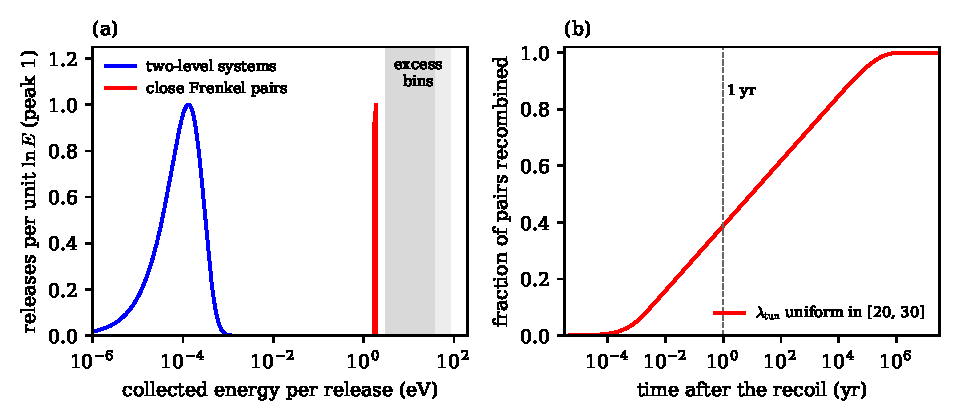
\includegraphics[width=\linewidth]{figures/ch19/fig19_5.pdf}
  \caption{Delayed releases from two defect families. (a) Distribution of the energy one release gives a sensor that absorbs a fraction $f_{\mathrm{ph}} = 0.25$ of the phonon energy, per unit logarithm of the energy, each family scaled to a peak of one. Blue: two-level systems frozen at $T_{\mathrm{frz}} = \SI{4.8}{K}$ and relaxing at \SI{10}{mK}, \cref{eq:19.6-tls}, mean quantum \SI{0.49}{meV}. Red: recombination of close Frenkel pairs in silicon, with configurational energies spread uniformly between 6.8 and \SI{7.5}{eV} (\cref{sec:7.4}), zero-point changes neglected. Gray: the 3--38 and 38--\SI{85}{eV} bins of energy absorbed in the sensor in which a glued silicon crystal shows its excess of events~\cite{anthonypetersen2024stress}. (b) Fraction of a family of close pairs recombined by time $t$, for strong coupling, $\varGamma = \SI{e13}{s^{-1}}\,\ee^{-2\lambda_{\mathrm{tun}}}$, with $\lambda_{\mathrm{tun}}$ spread uniformly between 20 and 30, an illustrative range around the two-parabola estimates. The fraction grows as $\ln t$ (a rate $\propto 1/t$) between \SI{6.5}{h} and $3.6\times10^5$ years; 0.39 of the pairs recombine within the first year. In the weak-coupling regime none does.}
  \label{fig:19-release}
\end{figure}

A close pair gives a sensor that absorbs a quarter of the phonons between 1.70 and \SI{1.88}{eV}, below the lowest bin of the excess (\cref{fig:19-release}(a)), and a two-level system gives a ten-thousandth of that. Single releases add to the heat load and, through the spectrum, to the noise of a sensor with a threshold of an eV or less; for thresholds of a few eV they are invisible. Amorphous pockets left by keV recoils are the one point-defect source that releases more at once: a pocket that recrystallizes releases of order \SI{0.1}{eV} per atom, an estimate, so a pocket of 120 atoms gives \SI{3}{eV} to such a sensor.

The inputs of these rates are computable from first principles. Barriers and minimum-energy paths come from the nudged elastic band, which relaxes a chain of configurations between the two minima onto the path, on the density-functional or machine-learned surface, the Huang--Rhys factors from the Hessians at both minima, and the exponent along the true path from ring-polymer instantons (\cref{app:E.22}). The sum rule \cref{eq:19.6-sumrule} is the acceptance test of the kinetic Monte Carlo, the stochastic sampling of hop sequences that turns the rates into $\mathcal{R}_{\mathrm{hop}}$.

\subsection{Defectons}\label{sec:19.6-defecton}

A light defect that tunnels between equivalent sites faster than the disorder around it can detune them becomes delocalized. This matters for a detector because a mobile defect reaches its partner, or a surface, on a time set by its band and not by a barrier. If the defect at site $\vect{r}$ tunnels to each neighbor with amplitude $A_{\mathrm{dfn}}$, the Bloch combinations of the localized states are stationary, and the defect becomes a quasiparticle, a defecton, with a band
\begin{equation}
  \varepsilon^{\mathrm{dfn}}(\vect{k}) = E^{\mathrm{loc}} - A_{\mathrm{dfn}}\sum_{i=x,y,z}\cos k_ia ,
  \label{eq:19.6-band}
\end{equation}
on a simple cubic lattice of spacing $a$~\cite[Eqs.~(1)--(3)]{pushkarov2004quantum}. The band width is $\Delta_{\mathrm{dfn}} = zA_{\mathrm{dfn}}$, with $z = 6$ neighbors, the mass at the bottom $1/A_{\mathrm{dfn}}a^2$, and the speed at most $A_{\mathrm{dfn}}a$. In solid helium, where defectons were first proposed, a ${}^3$He impurity has $\Delta_{\mathrm{dfn}} \sim \SI{e-4}{K}$; the light interstitials of metals, hydrogen in niobium for example, are candidates in the materials of detectors~\cite{pushkarov2004quantum}. In a hop the defecton cannot change its energy by more than $\Delta_{\mathrm{dfn}}$, so a gradient of the potential energy $\phi$ with $|\nabla\phi|a > \Delta_{\mathrm{dfn}}$ localizes it~\cite[Eq.~(17)]{pushkarov2004quantum}. Around a defect whose elastic interaction falls as $\phi = V_0(a/r)^3$, the gradient criterion reads $3V_0(a/r)^4 > \Delta_{\mathrm{dfn}}$, and the region $r < R_0 = a(3V_0/\Delta_{\mathrm{dfn}})^{1/4}$ is closed to band motion.

In a perfect crystal at $\Delta_{\mathrm{dfn}} \ll T$ the defecton moves through the band ballistically between collisions with phonons, and its diffusion constant falls as $T^{-9}$. The exponent follows from four facts: the kinematics of a narrow band, the Rayleigh form of two-phonon scattering, the small momentum change per collision, and the band velocity. First, the defecton cannot absorb or emit one phonon: that needs $|\varepsilon^{\mathrm{dfn}}(\vect{k} + \vect{Q}) - \varepsilon^{\mathrm{dfn}}(\vect{k})| = \bar cQ$, and the left side is at most $A_{\mathrm{dfn}}aQ$, far below $\bar cQ$ for a narrow band. The leading process is therefore two-phonon scattering, $\vect{Q} \to \vect{Q}'$ with $\omega' \simeq \omega$. Second, its amplitude is proportional to $\omega$. For a coupling quadratic in the strain, the elastic inhomogeneity of the defect, the amplitude carries $QQ'/(\omega\omega')^{1/2} \propto \omega$. The linear deformation coupling at second order has two time orderings with energy denominators $\pm\omega$ that cancel at leading order, and what remains is the second difference of the band, $\propto A_{\mathrm{dfn}}a^2QQ'$, again $\propto\omega$. The cross-section is therefore $\propto (Qa)^4$, Rayleigh scattering~\cite[Eq.~(49)]{pushkarov2004quantum}. Third, the number of thermal phonons grows as $T^3$, so the collision rate grows as $T^7$; but each collision changes the crystal momentum by at most about $T/\bar c$, much less than $1/a$~\cite[Eq.~(54)]{pushkarov2004quantum}, and $(1/Qa)^2 \propto T^{-2}$ collisions are needed to randomize it. The transport rate grows as $T^9$. Fourth, $D = v^2\tau_{\mathrm{tr}}/3$ with $v \sim A_{\mathrm{dfn}}a$ gives $D \propto \Delta_{\mathrm{dfn}}^2T^{-9}$. Pushkarov computes the rate of growth of the mean squared crystal momentum,
\begin{equation}
  \varGamma_{k^2} \equiv \frac{\dd\langle(\Delta\vect{k})^2\rangle}{\dd t} = \alpha_{\mathrm{P}}\,\sigma_{\mathrm{P}}\,\frac{\bar c}{a^3}\Bigl(\frac{T}{\theta_p}\Bigr)^9 , \qquad
  \theta_p = \frac{\bar c}{2a} , \qquad \alpha_{\mathrm{P}} = \frac{\pi^5\zeta(9)}{240\,\zeta(8)} = 1.27 ,
  \label{eq:19.6-q2}
\end{equation}
where $\bar c = (c_{\mathrm{LA}}^{-4} + 2c_{\mathrm{TA}}^{-4})^{-1/4}$ is his average sound speed and $\sigma_{\mathrm{P}}$ the strength of the defect's elastic perturbation relative to that of a vacancy~\cite[Eqs.~(48), (58)]{pushkarov2004quantum}. The characteristic temperature is $\theta_p$, about an eighth of the Debye temperature.

These four facts fix the exponent; the prefactor needs the motion in the band. Since each collision changes $\vect{k}$ by a small step, $\vect{k}$ diffuses, with $D_1 = \varGamma_{k^2}/6$ per Cartesian component, and detailed balance at temperature $T$ adds the drift $-D_1\nabla_{\vect{k}}\varepsilon^{\mathrm{dfn}}/T$. The band \cref{eq:19.6-band} is a sum over components, so each component moves on its own circle $\vartheta = k_xa$, with velocity $v_x = A_{\mathrm{dfn}}a\sin\vartheta$. The diffusion constant is the time integral of the velocity correlation, $D = \int_0^\infty\dd t\,\langle v_x(0)v_x(t)\rangle$. It equals $(A_{\mathrm{dfn}}a)^2\langle\sin\vartheta\,\chi\rangle$, where $\chi$ solves the backward equation $a^2D_1(\chi'' - U'\chi') = -\sin\vartheta$ with $U = -(A_{\mathrm{dfn}}/T)\cos\vartheta$, and the average is over $\ee^{-U}$. With $y = A_{\mathrm{dfn}}/T$, one integration gives $\ee^{y\cos\vartheta}\chi' = \ee^{y\cos\vartheta}/(ya^2D_1) + C$, and periodicity of $\chi$ fixes $C = -1/[ya^2D_1I_0(y)]$, with $I_0$ the modified Bessel function. An integration by parts then gives $\langle\sin\vartheta\,\chi\rangle = [1 - I_0(y)^{-2}]/(y^2a^2D_1)$, and
\begin{keyresult}[Defecton diffusion in a phonon gas]
\begin{equation}
  D = \frac{6T^2}{\varGamma_{k^2}}\Bigl[1 - I_0\Bigl(\frac{A_{\mathrm{dfn}}}{T}\Bigr)^{-2}\Bigr]
  \;\xrightarrow{\;T \gg \Delta_{\mathrm{dfn}}\;}\; D_9 = \frac{3A_{\mathrm{dfn}}^2}{\varGamma_{k^2}} = \frac{\Delta_{\mathrm{dfn}}^2}{12\varGamma_{k^2}} \propto T^{-9} .
  \label{eq:19.6-D}
\end{equation}
\end{keyresult}
\noindent At $T \ll A_{\mathrm{dfn}}$ the bracket tends to one and $D = 6T^2/\varGamma_{k^2} \propto T^{-7}$, the diffusion of a particle of mass $1/A_{\mathrm{dfn}}a^2$ with the friction that the same phonons exert. These are the two limits of Pushkarov's interpolation~\cite[Eqs.~(61), (64)]{pushkarov2004quantum}.

\begin{limitbox}[Defecton diffusion][lim:19.6a]
The published law is $D_T = (a\bar c/3\alpha_{\mathrm{P}}\sigma_{\mathrm{P}})[\varepsilon(p)/\theta_p]^2(\theta_p/T)^9$, for $\Delta_{\mathrm{dfn}} \ll T \ll \theta_p$~\cite[Eq.~(61)]{pushkarov2004quantum}, which is $D_9$ of \cref{eq:19.6-D} with $\varepsilon(p) = \Delta_{\mathrm{dfn}}/4$.
\par\smallskip
{\centering
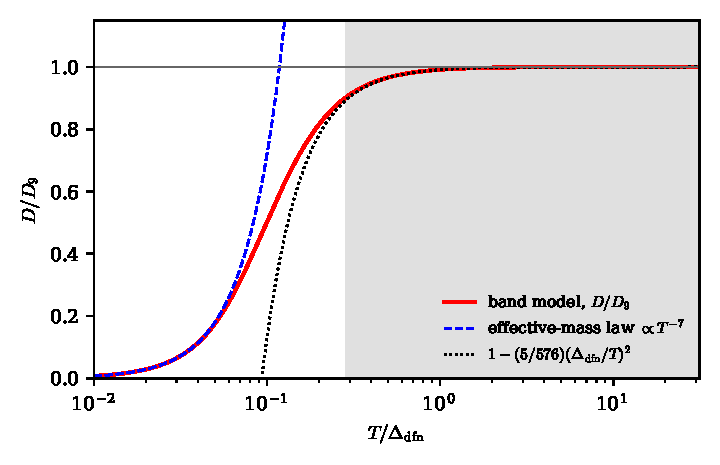
\includegraphics[width=0.75\linewidth]{figures/ch19/limit19_6a.pdf}
\captionof{figure}{Diffusion constant of a defecton in a simple cubic tight-binding band, \cref{eq:19.6-D}, divided by its $T^{-9}$ limit $D_9$, against the temperature in units of the band width. The ratio depends on $T/\Delta_{\mathrm{dfn}}$ alone, since the phonon rate $\varGamma_{k^2}$ of \cref{eq:19.6-q2} cancels. Red: the band model, crystal momentum diffusing at a constant rate with the detailed-balance drift. Blue dashed: the effective-mass law $D = 6T^2/\varGamma_{k^2} \propto T^{-7}$. Dotted: the leading correction $1 - \tfrac{5}{576}(\Delta_{\mathrm{dfn}}/T)^2$. Gray: within \SI{10}{\percent} of the $T^{-9}$ law, $T \ge 0.28\,\Delta_{\mathrm{dfn}}$. The upper edge $T \ll \theta_p$ lies outside the plot and depends on the crystal.}\label{fig:19-limit-defecton}
\par}
\smallskip
Below $0.28\,\Delta_{\mathrm{dfn}}$ the band is no longer uniformly populated and the law steepens toward $T^{-7}$; above $\theta_p$ the phonons are no longer long-wave and the Rayleigh law of the cross-section fails.
\end{limitbox}

The $T^{-9}$ law holds better than its derivation suggests. The ratio $D/D_9$ expands as $1 - (5/16)(A_{\mathrm{dfn}}/T)^2$, so the law is within \SI{10}{\percent} for $T \ge 0.28\,\Delta_{\mathrm{dfn}}$ and within \SI{1}{\percent} for $T \ge 0.93\,\Delta_{\mathrm{dfn}}$, although the condition stated with it is $T \gg \Delta_{\mathrm{dfn}}$. The relevant energy is the hopping amplitude, a sixth of the band width. At $T = 0.1\,\Delta_{\mathrm{dfn}}$ the local exponent is $-7.9$. A defecton moves faster the colder the crystal, until strain gradients localize it. In a real crystal the gradients from impurities, dislocations and the defect's own partner set $R_0$, and a band narrower than the elastic interaction at a few lattice spacings never carries the defect far.

\subsection{Crowdions}\label{sec:19.6-crowdion}

An extra atom in a close-packed row of a body-centered cubic metal spreads over many neighbors as a kink in the row, a crowdion. In tungsten, the metal of many transition-edge sensors, the self-interstitial takes this form along $\langle111\rangle$~\cite{fitzgerald2018structure}. The Frenkel--Kontorova chain of \cref{app:C.20} describes it: atoms of mass $M_\kappa$ at spacing $a_{\mathrm{ch}}$, springs $K_{\mathrm{ch}}$, and the potential $V_{\mathrm{s}}\sin^2(\pi z/a_{\mathrm{ch}})$ of the surrounding crystal, \cref{eq:C.20-FK}. For a slowly varying displacement the chain obeys the sine-Gordon equation, and its kink has the profile \cref{eq:C.20-kink} of width $d_{\mathrm{kink}} = a_{\mathrm{ch}}^2[K_{\mathrm{ch}}/2\pi^2V_{\mathrm{s}}]^{1/2}$~\cite[Eq.~(2)]{fitzgerald2018structure} and the rest energy $E_{\mathrm{kink}} = 4V_{\mathrm{s}}d_{\mathrm{kink}}/a_{\mathrm{ch}}$ of \cref{eq:C.20-Ekink}~\cite[Eq.~(3)]{fitzgerald2018structure}. The crowdion moves as a particle of mass
\begin{equation}
  M_{\mathrm{cr}} = \frac{2}{\pi^2}\,\frac{a_{\mathrm{ch}}}{d_{\mathrm{kink}}}\,M_\kappa ,
  \label{eq:19.6-Mcr}
\end{equation}
the kink mass \cref{eq:C.20-mass}~\cite{braun2004frenkel}, and the discrete row makes it cross the Peierls--Nabarro barrier $E_{\mathrm{PN}}$ of \cref{eq:C.20-EPN} to move by one spacing.

For tungsten, $V_{\mathrm{s}} \approx \SI{1}{eV}$ and $K_{\mathrm{ch}}a_{\mathrm{ch}}^2 = 50$ to \SI{100}{eV} are typical values~\cite{fitzgerald2018structure}. They give $d_{\mathrm{kink}} = 1.59$ to $2.25\,a_{\mathrm{ch}}$, $E_{\mathrm{kink}} = 6.4$ to \SI{9.0}{eV}, $M_{\mathrm{cr}} = 0.127$ to $0.090\,M_\kappa$ and a barrier of $1.2\times10^{-4}$ to $3.6\times10^{-7}\,\si{eV}$, with $a_{\mathrm{ch}} = \frac{\sqrt3}{2}\times\SI{3.165}{\angstrom} = \SI{2.741}{\angstrom}$. Atomistic calculations put the barrier near a meV instead~\cite{fitzgerald2018structure}, because the real substrate potential of tungsten is not a single sine. A particle of mass $M_{\mathrm{cr}}$ in the periodic potential $\tfrac12E_{\mathrm{PN}}[1 - \cos(2\pi z_0/a_{\mathrm{ch}})]$ has a ground band whose width follows from Mathieu's equation. The free-recoil energy $\pi^2/2M_{\mathrm{cr}}a_{\mathrm{ch}}^2$ is \SI{0.12}{meV} for the narrower kink, equal to its barrier within \SI{3}{\percent}, and \SI{0.17}{meV} for the wider one, and the band is 90 to \SI{166}{\micro eV}, 1.0 to \SI{1.9}{K}. With the atomistic barrier of \SI{1}{meV} and the same masses it narrows to 13 to \SI{34}{\micro eV}, 0.15 to \SI{0.39}{K}. Either way the band is wider than the temperature of a detector, so a crowdion is a candidate for coherent motion at millikelvin, a defecton of one dimension.

\begin{limitbox}[Crowdion profile and kink mass][lim:19.6b]
The published crowdion is the sine-Gordon kink \cref{eq:C.20-kink} with rest energy \cref{eq:C.20-Ekink}~\cite[Eqs.~(2), (3)]{fitzgerald2018structure}, of mass \cref{eq:19.6-Mcr} and barrier \cref{eq:C.20-EPN}.
\par\smallskip
{\centering
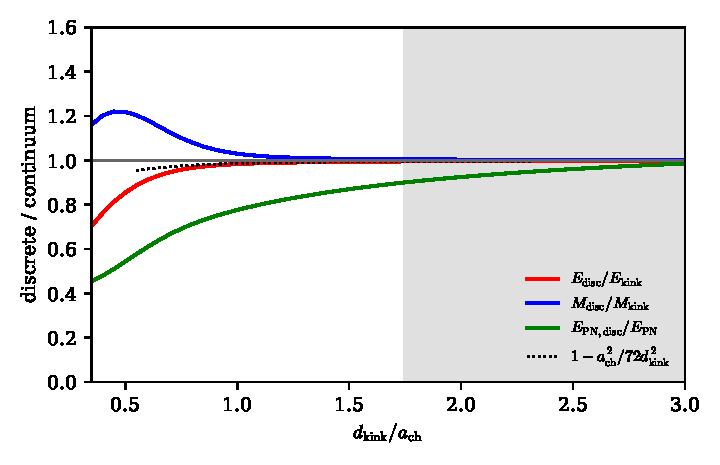
\includegraphics[width=0.75\linewidth]{figures/ch19/limit19_6b.pdf}
\captionof{figure}{Discrete Frenkel--Kontorova crowdion against the continuum kink, as ratios, against the kink width in units of the row spacing. The discrete chain of \cref{eq:C.20-FK} is relaxed numerically with the kink centered between two atoms (the minimum) and on an atom (the saddle). Red: rest energy, against $E_{\mathrm{kink}}$. Blue: translation mass $M_\kappa\sum_n(u_{n+1} - u_n)^2/a_{\mathrm{ch}}^2$, the lattice form of $M_\kappa\sum_n(\partial u_n/\partial z_0)^2$, against \cref{eq:19.6-Mcr}. Green: saddle minus minimum, against $E_{\mathrm{PN}}$ of \cref{eq:C.20-EPN}. Dotted: the leading correction to the energy, $1 - a_{\mathrm{ch}}^2/72d_{\mathrm{kink}}^2$. Gray: all three within \SI{10}{\percent}, $d_{\mathrm{kink}} \ge 1.74\,a_{\mathrm{ch}}$, set by the barrier.}\label{fig:19-limit-crowdion}
\par}
\smallskip
Well below one row spacing the kink is no longer a smooth profile: the barrier falls to half the continuum value near $0.4\,a_{\mathrm{ch}}$, and the mass and energy deviate by tens of percent.
\end{limitbox}

The energy and the mass of the kink hold far beyond the barrier. Replacing the spring energy $\frac12K_{\mathrm{ch}}\sum(u_{n+1} - u_n)^2$ by its continuum form drops the next term of $4\sin^2(ka_{\mathrm{ch}}/2) = k^2a_{\mathrm{ch}}^2 - k^4a_{\mathrm{ch}}^4/12$, which is $-(K_{\mathrm{ch}}a_{\mathrm{ch}}^3/24)\int\dd z\,u''^2$. On the kink, $\int\dd z\,u''^2 = 2a_{\mathrm{ch}}^2/3\pi^2d_{\mathrm{kink}}^3$, and to first order the energy changes by $-K_{\mathrm{ch}}a_{\mathrm{ch}}^5/36\pi^2d_{\mathrm{kink}}^3 = -E_{\mathrm{kink}}\,a_{\mathrm{ch}}^2/72d_{\mathrm{kink}}^2$, \SI{1.4}{\percent} at $d_{\mathrm{kink}} = a_{\mathrm{ch}}$. The discrete energy follows this law within $2\times10^{-4}$ above $1.5\,a_{\mathrm{ch}}$, and the mass exceeds \cref{eq:19.6-Mcr} by \SI{3}{\percent} at one spacing and by less beyond. The barrier is the weak point, \SI{22}{\percent} below \cref{eq:C.20-EPN} at $d_{\mathrm{kink}} = a_{\mathrm{ch}}$ and \SI{7.5}{\percent} below at $2\,a_{\mathrm{ch}}$, because it is exponentially small and the relaxation of the discrete chain changes it at the same order. For tungsten the model lies inside the shaded region for the stiffer chain and just below its edge for the softer one, so the mass is reliable and the barrier is not, as the atomistic meV already shows.

The conduction electrons, the phonons and the strain field of the parent vacancy decide whether the band survives in a real metal. Bulk tungsten is a normal metal above about \SI{15}{mK}, so its conduction electrons dress the hopping by a power of the ohmic coupling $\alpha_{\mathrm{ohm}}$ and, for $\alpha_{\mathrm{ohm}} < 1/2$, damp the coherent motion above a temperature of order $\Delta_{\mathrm{r}}/\pi\alpha_{\mathrm{ohm}}$, with $\Delta_{\mathrm{r}}$ the renormalized tunneling amplitude of \cref{sec:16.8-ohmic}. The phonons that distinguish neighboring positions multiply the hopping by $\ee^{-S_{\mathrm{pol}}(T)}$ of \cref{eq:E.22-Spol}, which has not been estimated for a crowdion. The strain field of the vacancy left behind confines the crowdion within $R_0$ of it: for an elastic interaction constant of about \SI{1}{eV}, an assumption, and a band of 13 to \SI{166}{\micro eV}, $R_0 = 12$ to 22 spacings. Inside $R_0$ the crowdion slides down the gradient toward its vacancy, and its recombination time is a drift time, peaked, not the $t^{-3/2}$ tail of a free random walk. The Peierls profile, the phonon coupling and the interaction with the parent vacancy remain to be computed with density-functional theory in a tungsten cell.

\subsection{The low-energy excess}\label{sec:19.6-lee}

Cryogenic detectors of many materials and designs record excess events whose spectra rise toward threshold, from tens of eV to a few keV~\cite{adari2022excess}. In the measurement of Anthony-Petersen and collaborators, two silicon crystals of $1\times1\times\SI{0.1}{cm^3}$, with identical sensors made on one wafer, were mounted in two ways: one glued to its copper holder with varnish, the other hung from aluminum wire bonds~\cite{anthonypetersen2024stress}. In energy absorbed by the sensor, the glued crystal shows a rate between 3 and \SI{38}{eV} more than two orders of magnitude above the suspended one. The rates in the 3--38 and 38--\SI{85}{eV} bins fall with time constants of 6 to 10 days after cooldown, while the rate above \SI{85}{eV}, from muons and radioactivity, stays constant. A single exponential does not describe the lowest bin of the glued crystal, with $\chi^2 = 4192$ for 68 degrees of freedom~\cite[Sect.~II\,B]{anthonypetersen2024stress}. In germanium detectors without a charge signal, the shape of the excess stays fixed while its rate falls slowly, the rate jumps after the detectors are warmed above \SI{10}{K}, and tests with adjustable stress on the crystal and different holders show no significant effect. One leading hypothesis there is the cracking of the epoxy that glues the thermistor to the crystal~\cite[Sect.~2.1.2]{adari2022excess}.

Energy conservation bounds what any defect source can supply, whatever the model. A source fed by particle events releases at most the energy those events stored, by \cref{eq:19.6-sumrule}: over any interval it releases the sum of $E_{\mathrm{st},k}(t_1) - E_{\mathrm{st},k}(t_2)$ over the events $k$ that seeded it. A source of elastic energy relaxing since cooldown releases at most the decrease of its relaxable elastic energy $U_{\mathrm{rel}}$. Point defects grown into the crystal or frozen in at cooldown release at most the decrease of their stored energy $E_{\mathrm{st},0}$, by the same sum rule. The energy recorded in excess events over $[t_1, t_2]$ obeys
\begin{multline}
  \int_{t_1}^{t_2}\dd t\int\dd E\;E\,\frac{\dd\mathcal{R}_{\mathrm{LEE}}}{\dd E\,\dd t}
  \le f_{\mathrm{ph}}\Bigl\{\bigl[U_{\mathrm{rel}}(t_1) - U_{\mathrm{rel}}(t_2)\bigr] + \bigl[E_{\mathrm{st},0}(t_1) - E_{\mathrm{st},0}(t_2)\bigr] \\
  + \sum_k\bigl[E_{\mathrm{st},k}(t_1) - E_{\mathrm{st},k}(t_2)\bigr]\Bigr\} ,
  \label{eq:19.6-leebound}
\end{multline}
with $f_{\mathrm{ph}} \le 1$ the largest collected fraction. The same bound holds for each event separately. Three consequences follow without any model: the event-seeded term is small, a single release must be large, and two crystals that differ in mounting differ in their elastic energy. First, electron recoils below \SI{0.14}{MeV} cannot displace atoms (\cref{sec:19.5-yield}), and a \SI{10}{eV} electron gives a silicon nucleus at most $4m_eE/M_\kappa = \SI{0.78}{meV}$. Nuclear recoils store at most \SI{5.5}{\percent} of their energy in silicon and \SI{6.4}{\percent} in germanium at \SI{95}{\percent} confidence (\cref{tab:19-bounds}). These bounds hold under the conditions of \cref{sec:19.5-yield}, and the silicon bound loosens to 0.081 at $\mathfrak{r}_{\mathrm{coll}} = 0.9$. Either way, the stored energy of the recoils a detector has seen is a small fraction of the energy it has already recorded from them. Second, at $f_{\mathrm{ph}} = 0.25$ an event of \SI{3}{eV} needs \SI{12}{eV} released at once, and one of \SI{38}{eV} needs \SI{152}{eV}, the energy of 22 close Frenkel pairs or of a pocket of about 1500 atoms. Third, two crystals cut from one wafer, with the same exposure to particles and the same grown-in defects, differ in mounting by $U_{\mathrm{rel}}$, provided that mounting changes neither $f_{\mathrm{ph}}$ nor the rates of stress-assisted defect reactions. The factor of more than a hundred between them then reflects elastic energy, not defects from radiation or growth. The excess events are therefore collective releases of energy stored at cooldown, and the open question is how they happen.

A collective-release model rests on three hypotheses: a reservoir of relaxable elastic energy, relaxation rates spread uniformly in $\ln\varGamma$, and a fixed law for the energies of single events. The reservoir $U_{\mathrm{rel}}$ is stored at cooldown in the crystal, the glue and the interfaces of the holder, and it relaxes by local events, thermally activated or tunneling, with rates between $\varGamma_{\min}$ and $\varGamma_{\max}$, spread as the barriers of a glass are (\cref{sec:16.8-heat}). We write the law of single-event energies as $p_{\mathrm{LEE}}(E)$. The second hypothesis fixes the time law by the argument of \cref{eq:16.8-heat}: the fraction relaxing per unit time is $1/[t\ln(\varGamma_{\max}/\varGamma_{\min})]$ for $\varGamma_{\max}^{-1} \ll t \ll \varGamma_{\min}^{-1}$, so each factor $\ee$ in time releases $U_{\mathrm{rel}}/\ln(\varGamma_{\max}/\varGamma_{\min})$. A fastest rate of order one per day bends the $1/t$ law at early times into the sum of exponentials that the data prefer. With $\langle E\rangle$ the mean of $p_{\mathrm{LEE}}$, the three together give
\begin{equation}
  \frac{\dd\mathcal{R}_{\mathrm{LEE}}}{\dd E\,\dd t} = \frac{f_{\mathrm{ph}}\,U_{\mathrm{rel}}}{\ln(\varGamma_{\max}/\varGamma_{\min})\,\langle E\rangle}\,\frac{p_{\mathrm{LEE}}(E)}{t} .
  \label{eq:19.6-lee}
\end{equation}
The size law comes from triggering. If the phonons of one release trigger on average $b_{\mathrm{br}}$ further releases, as in \cref{sec:16.8-open}, and the number triggered is Poisson, the total number $N_{\mathrm{casc}}$ in one cascade follows the Borel distribution
\begin{equation}
  P(N_{\mathrm{casc}}) = \frac{\ee^{-b_{\mathrm{br}}N_{\mathrm{casc}}}\,(b_{\mathrm{br}}N_{\mathrm{casc}})^{N_{\mathrm{casc}} - 1}}{N_{\mathrm{casc}}!} ,
  \label{eq:19.6-borel}
\end{equation}
with mean $1/(1 - b_{\mathrm{br}})$. By Stirling's formula it falls as $N_{\mathrm{casc}}^{-3/2}\ee^{-N_{\mathrm{casc}}(b_{\mathrm{br}} - 1 - \ln b_{\mathrm{br}})}$, a power law $N_{\mathrm{casc}}^{-3/2}$ cut off at $N_{\mathrm{casc}} \sim 2/(1 - b_{\mathrm{br}})^2$ near the critical value $b_{\mathrm{br}} = 1$. Such a cascade of elementary releases produces a spectrum that rises toward threshold as a power with an exponential cutoff.

The model predicts how the excess scales, not its rate. The rate is proportional to $U_{\mathrm{rel}}$, which for a layer under thermal-mismatch stress $\sigma_{\mathrm{str}}$ is of order $\sigma_{\mathrm{str}}^2\Vol/Y_{\mathrm{mod}}$ of the relaxing component, with $Y_{\mathrm{mod}}$ its Young's modulus. A glue layer on a clamped crystal dominates, and the factor of a hundred between glued and suspended crystals is a ratio of $U_{\mathrm{rel}}$ that a thermo-elastic calculation can test. The clock restarts when the relaxing component is warmed above the temperature at which it creeps, as in the jumps after warming above \SI{10}{K}. A stress applied to the bulk of a crystal that does not creep adds little $U_{\mathrm{rel}}$, which agrees with the null results under adjustable stress if the source lies in the glue of the thermistor. The shape of the spectrum and its time dependence factorize, so the shape does not change as the rate falls, as observed in germanium. A rate needs two inputs that do not exist: $U_{\mathrm{rel}}$ with its spread of rates $[\varGamma_{\min}, \varGamma_{\max}]$ for a given holder and glue, and the branching ratio $b_{\mathrm{br}}$, which fixes the size law. The first comes from a finite-element calculation of the cooldown stress with measured elastic and expansion data, with the relaxable fraction from low-temperature mechanical data of the glue. The second comes from the catalogue of release paths and the transport of the phonon pulse of one release. A fit of \cref{eq:19.6-lee} with these inputs to a glued and an unglued crystal would then have no free parameter.

\subsection{Open problems}\label{sec:19.6-open}

The release of close Frenkel pairs in silicon and germanium, and of split interstitials in aluminum, at millikelvin (\cref{sec:19.6-kinetics}) needs one calculation per path: the tunneling exponent along the computed minimum-energy path and $E_{\mathrm{reorg}}/\varepsilon^{\mathrm{hop}}$, both to about \SI{5}{\percent}.

In ionic crystals the electronic route to stored energy is prompt. A self-trapped exciton can turn into a close pair of an F center and an interstitial within picoseconds. Part of the energy of an electron recoil is then stored before the partition time, and the electron-recoil calibration of such crystals has a heat deficit too. Per unit deposit the stored energy is the number of excitons per unit energy times the conversion probability, the survival probability of the close pair and its configurational energy. The conversion probability at millikelvin and the survival of the close pair against tunneling recombination are not known.

Carriers of later events can drive defect reactions without heat. A capture or recombination at a defect puts energy into its local modes, and if the reaction coordinate is coupled linearly with Huang--Rhys factor $S_{\mathrm{HR,rxn}}$ and energy $\omega_{\mathrm{rxn}}$, the number of quanta it receives at $T = 0$ is Poisson (\cref{eq:5.6-poisson}). The probability that one capture drives the reaction over a barrier $V_{\mathrm{b}}$ is the tail
\begin{equation}
  p_{\mathrm{rxn}} = \sum_{n \ge V_{\mathrm{b}}/\omega_{\mathrm{rxn}}}\ee^{-S_{\mathrm{HR,rxn}}}\,\frac{S_{\mathrm{HR,rxn}}^n}{n!} ,
  \label{eq:19.6-prxn}
\end{equation}
and the stimulated rate is the capture rate times $p_{\mathrm{rxn}}$. It enters \cref{eq:19.6-master} as a time-dependent rate, so \cref{eq:19.6-sumrule} still holds. The Huang--Rhys factor, the mode energy and the barrier of real defects, with the change of charge state, are not computed.

\subsection{Uncertainty budget of the nuclear-recoil response}\label{sec:19.6-budget}

\Cref{tab:19-nuisances} collects the truncations and inputs of the chapter with their sizes.
\begin{table}[tbp]
  \caption{Uncertainty budget of the low-energy nuclear-recoil response. Classes and bases as in \cref{tab:10-nuisances}; ``delayed'' moves energy in time without changing the prompt yield.}
  \label{tab:19-nuisances}
  \centering\scriptsize\setlength{\tabcolsep}{3pt}
  \begin{tabular}{@{}>{\raggedright\arraybackslash}p{0.26\linewidth}>{\raggedright\arraybackslash}p{0.12\linewidth}>{\raggedright\arraybackslash}p{0.35\linewidth}>{\raggedright\arraybackslash}p{0.09\linewidth}>{\raggedright\arraybackslash}p{0.10\linewidth}@{}}
    \toprule
    Truncation or input & Type & Size & Basis & Section \\
    \midrule
    Classical propagation of the kicked Wigner ensemble & tilt & misses the third cumulant (share $\propto x_R^{-1/2}$) and quantum effects after the kick & computed & \cref{sec:19.1} \\
    Regime boundaries of the recoil dynamics & threshold & silicon 0.41, \SI{0.54}{eV}; 12.5--\SI{36}{eV}; 0.87--\SI{4.6}{keV}, at a criterion of 0.1 & est. & \cref{sec:19.1} \\
    Machine-learned surface along the recoil path & threshold; normali\-zation & thresholds to the \SI{0.7}{eV} step width; a few tenths of an eV per defect & input spread & \cref{sec:19.1} \\
    Charge below the binary threshold & normali\-zation; threshold & silicon yield 0.10 at \SI{100}{eV}; close-collision kernel not computed & unsized & \cref{sec:19.2} \\
    Migdal part of a measured yield & normali\-zation & 2.3--$4.4\times10^{-4}$ in $Y_q$, at most \SI{0.4}{\percent} at \SI{100}{eV} & computed & \cref{sec:19.2} \\
    Lindhard quenching below a few keV & normali\-zation & data 8--\SI{38}{\percent} below the formula at 0.1--\SI{3.9}{keV}; soft-collision continuation $+$\SI{13}{\percent} at \SI{1}{keV} & input spread; model & \cref{sec:19.3} \\
    Prefactor of the displacement count & normali\-zation & 0.70 (screened) against 0.8 (formula) and 1 (hard spheres) & computed & \cref{sec:19.4} \\
    Stored share of a nuclear recoil & normali\-zation (heat) & at most 0.055 (Si; 0.049 with the measured pair energy) and 0.064 (Ge), \SI{95}{\percent} C.L., under (a)--(e); Si 0.081 at $\mathfrak{r}_{\mathrm{coll}} = 0.9$ & input spread & \cref{sec:19.5} \\
    Gap energy unreturned in the read window & normali\-zation (heat) & $Y_{\mathrm{ph}}(0) = 1.407$ at \SI{100}{eV} with none returned; \SI{1}{\percent} needs at most 3.5--\SI{4.1}{\percent} unreturned & computed & \cref{sec:19.5} \\
    Collection ratio of Luke phonons & normali\-zation & 1.128 alone reproduces the silicon datum; transport estimate 0.81--1.02 & computed & \cref{sec:19.5} \\
    Pair energy adopted by the reconstruction & normali\-zation & $-0.0064$ in $Y_{\mathrm{ph}}$ at \SI{4}{V}, growing with bias & computed & \cref{sec:19.5} \\
    Collection offset from recombination phonons & normali\-zation & $\rho_g - 1 = 0.21$ gives the silicon deficit beyond the pair-energy offset & est. & \cref{sec:19.5} \\
    Collection ratio constant between two biases & normali\-zation & residual $(\dd\mathfrak{r}_{\mathrm{coll}}/\dd V_{\mathrm{bias}})\Delta V_{\mathrm{bias}}$ & unsized & \cref{sec:19.5} \\
    Zero-point change of the defect basins & normali\-zation (heat) & below \SI{0.1}{eV} per defect; widens the bounds by about $10^{-3}$ & est. & \cref{sec:19.5} \\
    Release of close pairs at millikelvin & delayed & frozen if weakly coupled; else needs an exponent 14 (Si) or \SI{6}{\percent} (Al) below the two-parabola value & est. & \cref{sec:19.6} \\
    Single releases in a phonon readout & new support & close pair 1.70--\SI{1.88}{eV} at a collected fraction of 0.25 & model & \cref{sec:19.6} \\
    Defecton and crowdion transport & delayed & $T^{-9}$ law within \SI{10}{\percent} for $T \ge 0.28\,\Delta_{\mathrm{dfn}}$; crowdion barrier $-$\SI{22}{\percent} at $d_{\mathrm{kink}} = a_{\mathrm{ch}}$ & model & \cref{sec:19.6} \\
    Rate of the low-energy excess & new support & relaxable elastic energy and branching ratio not computed & unsized & \cref{sec:19.6} \\
    \bottomrule
  \end{tabular}
\end{table}

\section*{Summary}

The nuclear response of \cref{chap:11} hands a recoil over to dynamics on the Born--Oppenheimer surface through one exact step: the Wigner function of the lattice with the momentum of the struck nucleus raised by $\vect{q}$ (\cref{sec:19.1}). In silicon the dynamics passes from quantum to classical at \SI{0.41}{eV}, leaves the harmonic regime near \SI{0.54}{eV}, displaces atoms from 12.5 to \SI{36}{eV} depending on direction, and excites electrons nonadiabatically from about \SI{0.9}{keV}. Below the displacement threshold a recoil deposits all of its energy as heat, which covers every electron-following recoil from dark matter lighter than about \SI{150}{MeV}.

A binary collision with a valence electron can bridge the gap only above $E_{R,\mathrm{th}} = (M_\kappa/m_e)\Eg^2/16E_{\mathrm{F}}$, \SI{352}{eV} in silicon and \SI{399}{eV} in germanium, yet the measured silicon yield shows no threshold down to \SI{100}{eV} (\cref{sec:19.2}). The Migdal part of the measured yield is at most \SI{0.4}{\percent} of the silicon yield at \SI{100}{eV}. Lindhard quenching is the limit with no stored energy, continuum stopping to zero speed and proportional conversion to pairs (\cref{sec:19.3}); the silicon data lie 8 to \SI{38}{\percent} below the formula between 0.1 and \SI{3.9}{keV}. Bethe stopping holds within \SI{10}{\percent} only above $1.84\,v_{\mathrm{F}}$, while silicon recoils move at 0.013 to $0.13\,v_{\mathrm{F}}$.

One balance law per event counts every share of the deposit once (\cref{sec:19.5}). A close Frenkel pair in silicon keeps 6.8 to \SI{7.5}{eV}, and the displacement count with a screened cross-section is 0.70 times the Kinchin--Pease value, against the 0.8 of the standard formula. Unit heat quenching requires that, within the read window, all gap energy has returned as phonons and no energy is stored. Under conditions on phonon collection, other missing energy and the pair energy of the reconstruction, the measured deficits of nuclear recoils bound the stored share at \SI{95}{\percent} confidence by 0.055 in silicon and by 0.064 in germanium. The silicon datum $Y_{\mathrm{ph}} = 0.952$ is reproduced either by a stored fraction of 0.042 or, with no stored energy, by a collection ratio of 1.128; at \SI{40}{V} the two readings differ by 0.028.

The stored energy is released after the partition time by tunneling (\cref{sec:19.6}). The release-path sum rule \cref{eq:19.6-sumrule} makes the energy released by all hops equal to the stored energy minus what is still stored, for any rates. A single release gives a sensor that absorbs a quarter of the phonons less than \SI{2}{eV}, and two-level systems give quanta of half a meV, so neither produces the excess events of tens of eV. Energy conservation bounds the low-energy excess by the stored energy of the events that seeded it and of the grown-in defects, plus the decrease of relaxable elastic energy, and the factor of a hundred between glued and suspended crystals places it in the elastic energy. The uncertainty budget of the chapter is \cref{tab:19-nuisances}. The charge, phonons and quasiparticles that the balance law leaves at the end of the read window are not yet a signal; the next chapter follows them to the sensors.

\printbibliography[heading=subbibliography]
